%!TEX TS-program = xelatex
%!TEX encoding = UTF-8 Unicode

\newcommand{\myscore}[2]{\mathit{sc}^{({#1})}({#2})}

% Load Thesis Class
\documentclass{DEIThesis}

\title{Design of a Third-Order Word Embedding Model Using Vector Projections}

\author{Ahmet Onur Akman}
\studentId{2044006}

% Advisor
\advisor{Prof. Giorgio Satta}

% If you are co-advised
\coadvisor{Prof. Augusto Ferrante}
\coadvisorsUniversity{University of Padova}

\coadvisortwo{Prof. Giorgio Maria Di Nunzio}
\coadvisorsUniversitytwo{University of Padova}

\university{University of Padova}
\mastername{Computer Engineering}
\academicYear{2022/2023}

\begin{filecontents*}[overwrite]{\jobname.xmpdata}
    \Title{Design of a Third-Order Word Embedding Model Using Vector Projections}
    \Author{Ahmet Onur Akman}
    \Language{en-EN}
    \Keywords{Computer Engineering\sep LaTeX}
\end{filecontents*}

% Document

\begin{document}
    % The front matter (Cover, ToC, Abstract, etc...)
    \frontmatter

    % The main content
    \mainmatter

    %!TEX root = ../main.tex

\chapter{Introduction}
\label{chp:intro}

In this chapter, we will draw a background for our study topic. First, we will have a brief overview of Machine Learning and some of its sub-fields and applications. We will present some further details about Deep Learning and give a blueprint for the training procedure of the Deep Learning models. Later, we will look closely at the purpose and sub-fields of Natural Language Processing, and the importance of word embeddings in particular. Building on this, in Chapter-\ref{chp:stateOfArt}, we will see some of the state-of-the-art embedding techniques, and how they differ from one another.


\section{Background: Machine Learning}

%\subsection{What is Machine Learning?}

\ac{ML} is an \ac{AI} sub-field focused on developing algorithms and statistical models that enable computer systems to learn from data, to gain the ability to make predictions or decisions, without the need for explicit programming of rules. These predictions or decisions can be described as a wide range of tasks, from the detection of a range of objects in the input images \cite{maskrcnn}, to estimating future stock prices based on a diverse set of variables \cite{stockmarket}.

Machine learning algorithms use mathematical and computational techniques to learn from data. These algorithms learn by tuning their parameters based on the training data to improve their performance as learning progresses. The direction in which parameters should be changed is determined by the target functions designated by the system designers. A machine learning model can operate on data in many formats, such as text, image, audio, strings of numbers, combinations of these, and many others. Unlike traditional software development paradigms, where rules and logic are programmed explicitly, machine learning systems derive their rules and logic from data. This enables them to carry out complex tasks for which it is difficult to clearly define the rules.

\subsection{Machine Learning: Use of data in learning}

\ac{ML} can be broken down into three main approaches, in terms of the use of the data. All \ac{ML}-related tasks can be said to employ one of the following paradigms in terms of the role of data in learning: \textbf{Supervised Learning}, \textbf{Unsupervised Learning}, or \textbf{Reinforcement Learning}. Even though it is possible to draw further branches from these paradigms, for now, this level of detail will be sufficient.

A \textbf{supervised} learning system learns under the assumption that there is a ground truth and the goal is to approximate it by tuning the internal parameters. This paradigm can be employed when the objective is to learn from a given set of decisions and imitate their thought process on new data later on. This is applicable for scenarios such as when the goal is to develop a computed tomography analyzer and there is a set of analyzed CT images available \cite{strokedet}, or if the goal is to create a system that can detect sarcasm in the text when a dataset of annotated text for this purpose is present \cite{sarcasmdet}.

\textbf{Unsupervised} learning, on the other hand, is suitable for making decisions or predictions on data, without the need to learn certain rules from a supervisor beforehand. Even though it is usually ideal to have a teacher to correct the mistakes of the system, eliminating the need for it can relieve the designers from the necessity of collecting and annotating a proper dataset. 

\textbf{Reinforcement} learning is a more distinct paradigm than the other two. It is rather about trial and error. The learning task is modeled as the process of learning a \textit{policy} that maps each possible \textit{state configuration} to \textit{actions}, in order to maximize a \textit{cumulative reward}. The learning agent is exposed to the \textit{environment} and able to manipulate it for a given number of \textit{episodes}, and the \textit{observations} made in progress are useful for the learning task. This is useful for tasks like motion learning of robotic arm manipulators \cite{robotRL}, or the development of a model that can play Atari games \cite{atariRL}, and many more.

\subsection{Deep Learning}

\ac{DL} is a sub-field of \ac{ML} that encompasses a class of \ac{ANN}s characterized by their depth. The main goal of deep learning is to automatically learn hierarchical representations of data.

The core of deep learning is \ac{ANN}s, specifically \ac{DNN}s, which consist of interconnected nodes, or \textit{neurons}, organized in \textit{layers}. These neurons are the building blocks of an \ac{ANN} and are responsible for calculations. Their input is provided by the neurons in the previous layer, and their output is the input of the neurons in the next layer. These input and output connections between neurons are associated with certain coefficients, called \textit{weights}. Neurons apply nonlinear operations using \textit{activation functions}, and this non-linearity is the factor that enables neural networks to solve more complex problems.

Generally, a \ac{DNN} consists of an input layer, one or more hidden layers, and an output layer. The input layer is where the network receives data, and the number of neurons depends on the format and shape of the input. Hidden layers, stacked between the input and output layers, are responsible for converting input data into increasingly more abstract representations. The output layer produces final predictions based on the representations learned in the previous layers. The architecture and number of nodes in this layer depend on the task, such as classification, regression, or generation. A simple feedforward neural network architecture is given in Figure \ref{fig:feedforward}.


\begin{figure}[ht]
    \begin{minipage}{\textwidth}
        \centering
        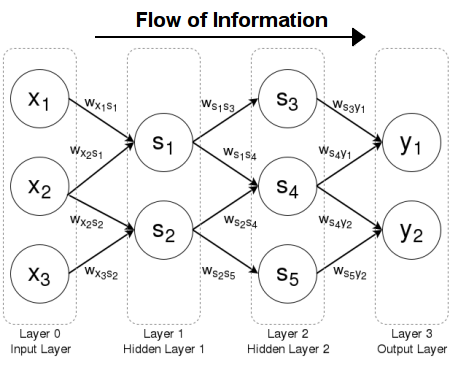
\includegraphics[width=0.5\textwidth]{img/feedforward_NN.png}
        \caption[A simple deep feedforward neural network with two hidden layers.]{A simple deep feedforward neural network with two hidden layers.\footnote{Source: \url{https://brilliant.org/wiki/feedforward-neural-networks/}}}
        \label{fig:feedforward}
    \end{minipage}
\end{figure}

Deep learning models are trained using large datasets and optimization techniques to adjust the weights and biases of connections between neurons. The complexity of the network is decided based on several factors, such as the complexity of the task, the size and proportion of training data, and the desired performance. This training process aims to minimize the error or loss function by effectively tuning the model's parameters to make accurate predictions on previously unseen data. Depending on the complexity of the tasks or the availability of certain types of samples in the data, training of deep models can get quite data-hungry.

The general architecture mentioned is valid for standard \ac{FNN}s, but many different architectures exist for different tasks and needs. Some of the most popular are \ac{CNN}, \ac{RNN}, \ac{GNN}, and \ac{LSTM}. For example, \ac{CNN}s are very useful for processing matrix-formatted input data, and \ac{RNN}s are designed for temporal data where previous input history is useful for decision-making.

\begin{figure}[ht]
    \begin{minipage}{\textwidth}
        \centering
        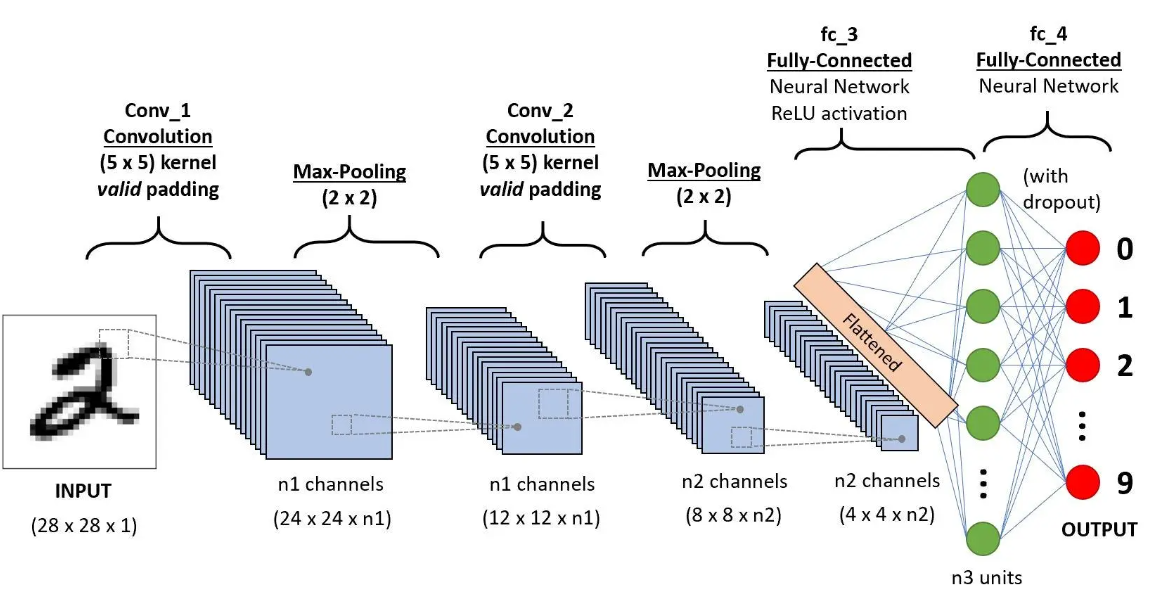
\includegraphics[width=0.8\textwidth]{img/cnn.png}
        \caption[A Convolutional Neural Network architecture for handwritten digit recognition.]{A Convolutional Neural Network architecture for handwritten digit recognition.\footnote{Source: \cite{CNNimg}}}
        \label{fig:cnn}
    \end{minipage}
\end{figure}

Deep learning models have achieved remarkable success in a variety of fields and provided solutions for a range of problems that were previously thought to be not solvable with computers. This is achieved thanks to the automatic discovery of complex patterns and representations from raw data.

\subsection{Training of a deep learning model}

Now we will have a closer look at the training procedure of \ac{DL} models. This way we will have an intuition about the training procedure of our word embedding model, which will be described later on.

The training procedure is essentially a systematic search for the optimal configuration of parameters. The optimality of a configuration is indicated by a target or a loss function. The optimal configuration is the configuration that maximizes the target function, or that minimizes the loss function. We will use the loss function in our descriptions. Therefore, the goal of the training is formulated as an optimization problem of the loss function. Building on this, the definition of the optimal parameter configuration \(\theta^*\) is:

\[ \theta^* = \arg\min_\theta \left[ \mathbb{E}[L(\hat{Y}, Y)] \right] \]

\noindent
where \(Y\) is the vector of the true target values, \(\hat{Y}\) is the model's predictions made with the configuration \(\theta\) for the input data, \(L\) is a function that measures the discrepancy between the model's predictions and the true labels.

The above definition is more accurate for a supervised learning setting, but loss-based optimization is also applicable to an unsupervised learning system. In this case, the loss is calculated only using the network predictions. We can generalize the definition as:

\[ \theta^* = \arg\min_\theta \left[ \mathbb{E}[L(Y)] \right] \]

In real-life scenarios, finding this optimal configuration is not always possible, therefore we usually settle with "close enough". We mentioned that this procedure is systematic, meaning it operates on a pipeline with a designated set of steps. Depending on the task, these steps do differ, however, we will try to list the ones that are somewhat common in all \ac{DL}-related tasks.

\textbf{Data Collection:} For the learning of a \ac{DL} model, the first thing to do is to create a dataset. With the increasing interest in \ac{AI} and \ac{DL}, this step is often omitted, since there is usually a dataset suitable for the majority of the tasks available online. When this is not the case, the creation of a dataset includes gathering data samples that are in the same format as the samples that the model will make predictions on after the training. These samples should be organized in a usable format, and if needed, missing and mistaken values should be handled. This procedure is often called \textit{data cleaning}. Afterward, if needed, the samples should go through steps of preprocessing before the training. These steps can be designed to prepare the samples for the training procedure or increase the training efficiency. For example, we needed to first tokenize our corpus, and it was needed for creating training batches. On the other hand, we also removed stop-words, but this was for capturing more contextual information. In the majority of the applications when the number of training samples is sufficient, the preprocessing also involves splitting the dataset into training, test, and validation sets. This is needed for training the model, monitoring its progress, and fairly evaluating its final performance by using a single dataset.

\textbf{Model Design:} The next thing is to design the model architecture. For \ac{ANN}s, this means deciding the number and types of layers, the number of neurons in each layer, and the activation functions. These are decided based on the type and the complexity of the task, the number of training samples available, and the shape of the input data. Once this is done, the weights of neuron connections are initialized. The most natural idea is the random initialization, but considering that this can greatly impact the training, this is yet another thing that the designer should be mindful of.

\textbf{Loss Function:} Loss function is one of the most important factors of the training procedure. The goal of training is modeled as the minimization of the loss function. Therefore, it is very important that the loss function accurately represents the goal of training. There are loss functions commonly used for different tasks, for example for regression, \ac{MSE} Loss is a common choice, or for binary classification \ac{CE} loss is commonly used. For the unsupervised setting, there are popular loss options such as \textit{inertia} for clustering tasks and \textit{autoencoder loss} for dimensionality reduction. For more specific tasks, the designer must design a custom loss function, representing the margin between the model's predictions and the true values.

\textbf{Optimizer:} The learning procedure is essentially iteratively updating the weights and bias of the network given the current loss. Updating these weights according to the direction and value indicated by the loss function is done by using an optimizer. The optimizer iteratively optimizes the parameters of the network using gradients. This gradient-based optimization of parameters in a single iteration can be formulated as:

\[
\theta_{k+1} = \theta_k - \alpha \nabla L
\]
\noindent
where \(\theta_k\) is the parameter vector at iteration $k$, \(\theta_{k+1}\) is the parameter vector at iteration $k+1$, \(\alpha\) is the learning rate (see Hyperparameters below), and \(\nabla L\) is the gradient of the loss with respect to the network parameters.

Different optimizers can do this operation in different ways, some update all parameters at once, while others work with batches (small subsets of data). Some make all updates according to the same learning rate, but some automatically find the appropriate learning rate for different parameters. Some of the most common optimizers are \ac{SGD}, Adam, and RMSprop.

\textbf{Hyperparameters:} Hyperparameters are parameters that shape the training procedure. They are not learned, in other words, the values assigned to them at the beginning of the training do not change throughout the training. There are many hyperparameters, but some of the most common are the number of epochs, batch size, and learning rate. The number of epochs is the number of times the entire training data passes through the entire network. Choosing the wrong epoch number might result in \textit{overfitting} or \textit{underfitting}. Batch size is the size of the groups to be used in the parameter update procedure. The wrong batch size will cause training to be too slow or introduce too much noise in learning. The learning rate is the step size of the parameter updates. A not-so-ideal learning rate can slow down the training or cause it not to converge to optimal values. It is common practice to run the training several times with different hyperparameter configurations and compare the results, as these have a direct impact on the final performance of the model and the ideal configuration is usually not very straightforward.

\textbf{Training Loop:} Once the training starts, we iterate over the training data in mini-batches. A mini-batch is a small subset of data. Working with mini-batches is a good balance between training with the entire dataset at once and going sample by sample. The motivation for this approach is to speed up the training by also reducing memory usage. 
At each step, for each mini-batch, we follow four steps.

\begin{enumerate}
  \item \textbf{Forward Pass:} Model makes predictions given the training data as the input.
  \item \textbf{Loss Computation:} Given the model predictions (and the true labels, if supervised), calculation of the discrepancy. 
  \item \textbf{Backpropagation:} Computation of the gradient of the loss with respect to the parameters of the network.
  \item \textbf{Parameter Update:} Based on the computed gradients, the optimizer adjusts model parameters in the direction that minimizes loss. The size of this adjustment is based on the gradient and the learning rate.
\end{enumerate}

These four steps are applied for the number of epochs for the entire training set. A good choice of the number of epochs yields a satisfactory training accuracy, but not by overfitting.
It is usually a good idea to monitor system performance throughout the training. This will be useful for fine-tuning the parameters and detecting overfitting early on. This can be done using a validation set, by monitoring the validation loss calculated using the labels of validation data and the model's predictions on them. It is very important to not include the validation samples in the training set. Once the training is completed, these results can be visualized to give a better perspective on the effectiveness of the training algorithm.

\textbf{Evaluation:} Once the training is completed, the model's performance is evaluated on unseen test samples. These samples can be taken from the same dataset or some other, but the main thing to pay attention to is that this data should not be seen by the model during the training. Based on the loss calculated with this test data, one can have a better idea about the generalization capability of the model. Common practice is to use metrics like \textit{recall}, \textit{precision}, and \textit{f1-score} when applicable.




\section{Background: Natural Language Processing}

Understanding \ac{NLP} and its significance is important as it underpins the motivation for exploring static word embeddings in this dissertation.

%\subsection{What is Natural Language Processing?}

\ac{NLP}, a sub-field of \ac{AI}, is dedicated to the medium of natural language, used in the human interactions. It enables machines to read, process, and derive meaning from text-formatted data. As the amount of text data gets larger, it contains more useful information, but it also gets more challenging to extract it. The emergence of \ac{NLP} was driven by the need for automated processing of data in text format, which is rapidly growing in size. 

\ac{NLP} made it possible to use the natural language for communication between humans and computer programs.  However, the natural languages used in human lives have a very complex nature, which makes it challenging to model and interpret them by our machines for mathematical calculations. Therefore, it all begins with the recognition that human language is large, inherently complex, and characterized by nuances, idiomatic expressions, and context-dependent senses.

\ac{NLP} is an interdisciplinary field that intersects with linguistics, computer science, artificial intelligence, statistics, and cognitive psychology. Its multifaceted nature allows researchers to approach the challenges using the knowledge collected in a range of research fields, to tackle a wide array of linguistic phenomena, ranging from syntax and semantics to pragmatics and discourse analysis.


\subsection{Why is Natural Language Processing Challenging?}
Despite its progress, \ac{NLP} faces numerous challenges due to the complexity of the natural languages. Some of these challenges are:

\begin{itemize}
\item Language interpretation is ambiguous.
\item Need to deal with a wide set of languages and their different dialects. Different languages not only have different words and phrases but also sometimes they differ greatly in their syntactics.
\item Even though it is usually straightforward for humans to recognize sarcasm, irony, and humor, it can be very tricky for computers.
\item Need to adapt to always-changing linguistic trends and cultural shifts. New trends might reduce the use of a common word, or introduce new words, new phrases, and different uses of the existing words.
\end{itemize}

Most of these challenges stem from the properties of natural languages. Such as:

\begin{itemize}
\item \textbf{Ambiguity}: It emerges in different scales. Sounds can have different transcriptions, words can have different senses and sentences can have different interpretations. 
\item \textbf{Compositionality}: The meaning of multi-element linguistic expressions is given by some function of the meaning of lower-level units and the way they are syntactically combined together.
\item \textbf{Recursion}: A language is based on some grammar. The rules of grammar can iterate on words to generate an infinite number of compositions, each with its specific meaning.
\item \textbf{Hidden Structure}: The language is believed to have a hidden structure, as any local change in a sentence can potentially disrupt the interpretation of the entire expression.
\end{itemize}

\subsection{Applications of NLP}

Thanks to the advancements in machine learning, \ac{NLP} studies have spread over a very wide scope due to its vast array of real-world applications, including:

\begin{itemize}

\item \textbf{Machine translation}, overcoming the language barriers for information exchange.
\item \textbf{Sentiment analysis}, revealing public sentiment towards products, services, artistic creations, political figures, ideas, events, and many more.
\item \textbf{Fake news detection}, protecting public opinion from misleading statements.
\item \textbf{Chatbots and virtual assistants}, enabling human-like interactions with machines.
\item \textbf{Question Answering}, automatically learning from existing data for more efficient learning from it by humans.
\item \textbf{Information retrieval}, for information extraction from unstructured and possibly large text formatted data.
\item \textbf{Text summarization}, condensing lengthy texts into concise summaries.
\item \textbf{Speech recognition}, converting speech into text.

\end{itemize}

These and many other applications of \ac{NLP} are beneficial for commercial use, but also handy in our personal lives. For commercial use, they enabled companies to optimize their operations and engage better with their customers, increasing their revenues in the scale of millions in some instances \cite{comm-nlp}. They also come in handy in many forms for us in our daily lives, such as auto-complete-supported digital keyboards, language model-supported smart search engines \footnote{As of today, the most known product: \url{https://www.bing.com}}, and smart home assistants.


\subsection{Background: Word embeddings}

Representation of words in a human mind is not applicable to today's machine learning algorithms, therefore we need another way of representing them. For this purpose, we use word embeddings, an appropriate representation of words that can be comprehended by machine learning algorithms. Word embeddings are the building blocks of \ac{NLP} applications. Essentially, an embedding of a word is a vector in a high-dimensional vector space, containing the semantic and syntactic characteristics of that word. Embeddings bridge the gap between the discrete nature of words and the continuous mathematical spaces. Representing a word as a high-dimension vector can implicitly encode rich linguistic information. This is a crucial property for almost all \ac{NLP} tasks, as it enables machines to learn and store not only the meaning of words but also the contextual associations between them. 

When we say word embeddings, usually we mean either one of two kinds of them. We will briefly introduce both, but for the rest of this dissertation, we will use the terms "Word Embeddings" and "Static Word Embeddings" interchangeably. 

\subsubsection{Static word embeddings}

Static word embeddings (also known as \textbf{pre-trained word embeddings}) are vector representations of words generated by learning from a large, static corpus. The name of these models suggests the fact that these embeddings are computed before the downstream \ac{NLP} task and cannot be modified once the learning phase is completed. Usually, static embeddings are computed with matrix factorization or shallow neural networks.

When used, the word embeddings are stored and accessed just like using a dictionary. Every \textbf{type} in the corpus corresponds to one unique vector and it is the same regardless of the context in which the word occurs. From this, it is easy to see that if a word is not present in the training corpus, the embedding model will not generate an embedding for it, and one needs to tackle this issue during the downstream task appropriately.

Static word embeddings are mostly based on the \textit{distributional hypothesis}, which says that words with similar meanings are likely to occur in similar contexts. In other words, within the corpus, words that are surrounded by similar words, or frequently co-occur with each other, should have similar meanings. Learning from a fixed corpus, these embeddings are designed to approximate the statistical patterns of word co-occurrence. For this approximation, different algorithms rely on different statistical measures, such as co-occurrence frequencies or \ac{PMI}, to determine the contextual relationships of words.

Even though they are more straightforward to train and easier to use, static embeddings usually fail to capture more fine-grained contextual characteristics of the words. A static word embedding model can be perfectly able to list the most similar and related words to a given word, but distinguishing different word senses is a difficult challenge even for the most popular static embedding models.

\subsubsection{Dynamic word embeddings}

Dynamic word embeddings (also known as \textbf{contextual word embeddings}) are context-aware word representations. These embeddings are generated dynamically for each \textbf{token} in the corpus based on the surrounding words in a given context. They are commonly trained using artificial neural networks (for example, \ac{ELMo} architecture uses a bi-directional \ac{LSTM} model \cite{elmo}), and transformers (\ac{BERT} is based on a multi-layer bidirectional transformer encoder \cite{bert}).

Dynamic word embeddings are generated by taking into account the neighboring words to a target word in a given context. They succeed in word sense disambiguation and context-dependent meanings.

Dynamic embeddings are closely related to the task of language modeling. Many language models rely on dynamic word embeddings to capture contextual characteristics and relationships of words. After the embeddings are learned from a large corpus, the vectors later can be conveniently fine-tuned in the pre-training of downstream \ac{NLP} task.










    %!TEX root = ../main.tex

\chapter{State of the Art}
\label{chp:stateOfArt}

Geometrical representations of words are the building blocks in the field of \ac{NLP}, for higher-level tasks such as word sense disambiguation, sentiment analysis, and language modeling. The efforts for developing static word embeddings go all the way back to the 1980s, and currently there are many models in the literature each approaching the problem with a different methodology.

In this chapter, we will list and briefly describe some of the most known static word embedding models. This background will be later useful to demonstrate how our approach differs from others.

\section{word2vec}

One work that established a fundamental step in the field of \ac{NLP} is word2vec, which was presented in the article \cite{w2v} by Tomas Mikolov, Kai Chen, Greg Corrado, and Jeffrey Dean. More precisely, in this article, the authors present a shallow neural network-based training of two different architectures, namely, \ac{CBOW} and \ac{SG}.

For each word in the vocabulary, word2vec produces a vector, which is typically of several hundred dimensions. The training procedure organizes the vector space in such a way that if two words share similar contexts, i.e. they are both surrounded by the same words, then the two vectors associated with them are close to each other. Consequently, similar words like “car” or “automobile”, or related terms, like “fork” and “spoon”, will have similar vectors, considering that they have similar contexts in the training corpus. 

\begin{figure}[h]
    \centering
    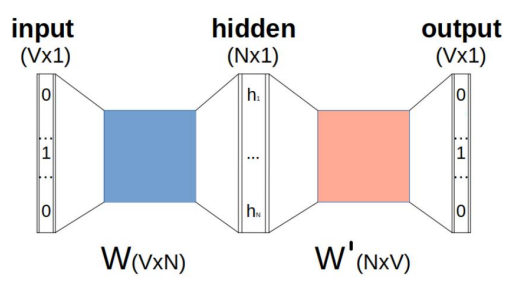
\includegraphics[width=0.8\textwidth]{img/g1.PNG}
    \caption{Generic word2vec architecture}
    \label{fig:g1}
\end{figure}

word2vec models are trained via an unsupervised approach, by feeding the neural network a large corpus with unannotated types in it. The network is trained with gradient descent to perform a particular task different from the one of interest. There is no activation function on the hidden neurons layer, and the output neurons use the softmax function. After training, the output layer is discarded, keeping only the input layer, which represents the target of interest. In this specific case, the network is trained to optimize an objective function to answer the question "Is the word $w$ likely to appear near the word $c$?". Subsequently, the input layer parameters will constitute the searched word embeddings.

\subsection{CBOW}

\ac{CBOW} model aims to train a neural network in such a way that it can predict a central word, given a fixed window of $2L$ words in its context. That is, if the system input is a text of a given length, consider $w_t$ the current central word (in the example “pepper”) and $w_i$ with $i = t - L, t - L + 1, ..., t + L - 1, t + L$ the words in its context, i.e. the words close to it in the corpus (in the example if $L = 2$, the context words are “cinnamon”, “salt”, “allspice” and “pine”), then the purpose of the model is to predict $w_t$ given $w_i$.

\begin{table}[!h]
\centering
\begin{tabular}{cccccccc}
seasoned & with & cinnamon, & salt, & pepper, & allspice, & pine & nuts \\
$w_{t-4}$ & $w_{t-3}$ & $w_{t-2}$ & $w_{t-1}$ & $w_{t}$ & $w_{t-+1}$ & $w_{t+2}$ & $w_{t+3}$
\end{tabular}
\end{table}

%To do this, the network is constructed as in Figure 3.2.

%\begin{figure}[h]
%    \centering
%    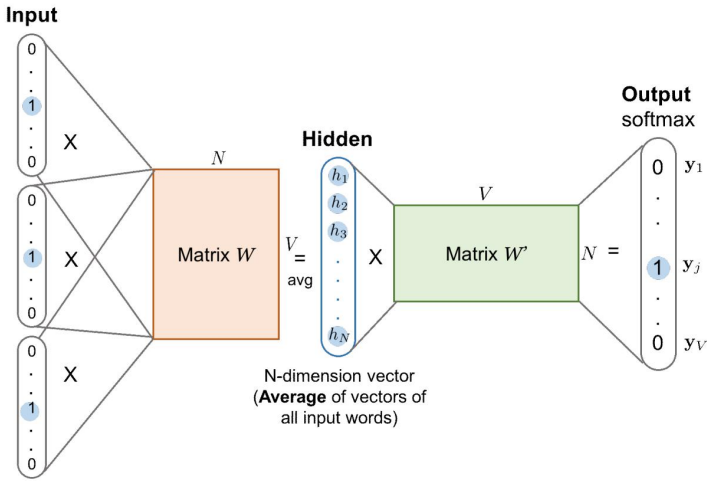
\includegraphics[width=0.95\textwidth]{img/g2.PNG}
%    \caption{CBOW architecture}
%    \label{fig:g2}
%\end{figure}

%This network has as input the 2L one-hot representations of the context words wi , each of 
The network constructed for this task has as input the $2L$ one-hot representations of the context words $w_i$, each of size $|V| \times 1$, with $|V|$ the size of the vocabulary. The hidden layer is composed of a vector $h$ of size $N \times 1$, with $N$ being the dimension of the word embeddings. The value of the hidden layer is calculated as the average of the vectors corresponding to the input context words transformed by the input weights matrix $W$., i.e.

\[
h = \frac{1}{2L}\sum_{i=-L, i \neq 0}^{L} x_{t-1}^{T} W_{(N \times |V|)}
\]

Subsequently, the product $W'h$ is calculated, where $W'$ is the matrix of hidden weights, obtaining a vector $z$ of dimension $|V| \times 1$. The output is then calculated from $z$ via the softmax function so that the output layer reports for each word $y_i$ in the vocabulary, the probability that it is the central term considering the context given in input. Finally, assuming that the node with the highest probability is $y_s$, the output one-hot vector will be the one with value $1$ in the $s$-th component and with all the remaining components set to 0.

%This model has as parameters two weight matrices W and Wÿ such that:

%\begin{itemize}
%    \item  W ÿ RN×|V | it is the matrix that will contain the embeddings of the words considered as central words
%    \item  Wÿ ÿ R|V |×N is the matrix that will contain the embeddings of the words considered as context words.
%\end{itemize}

Once the training is complete, the rows of matrix $W$ will be the desired word embeddings, corresponding to each word in the vocabulary.


\subsection{Skip-Gram}

Now we focus on how the Skip-Gram model works. Starting from a word in the middle of a sentence, called the \textit{central word}, consider the words surrounding it within a $2L$-sized window, called \textit{context words}. Differently from \ac{CBOW}, this model aims to predict the context words starting from the central word through the optimization of an objective function. The model scheme is represented in Figure \ref{fig:g3}.

\begin{figure}[h]
    \centering
    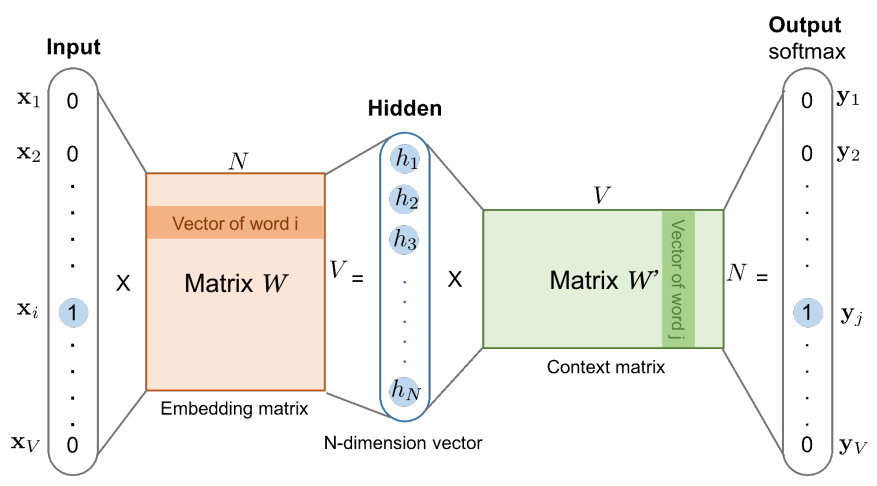
\includegraphics[width=0.95\textwidth]{img/g3.PNG}
    \caption{Skip-Gram architecture}
    \label{fig:g3}
\end{figure}

We see that the model input is a one-hot vector $x$, of dimension $|V| \times 1$, pointing to the current central word $w_t$. The output of the network consists of a single vector containing a probability distribution on all the vocabulary items, where each component represents how probable it is to find the corresponding vocabulary word in the vicinity of the central word.

%An important assumption is that given a central word, the various context words are completely independent %and identically distributed between them (iid). In other words, all the words within the considered window %are treated in the same way with respect to the input word, i.e. different sets of probabilities are not %learned based on the distance from the input.

Similarly to \ac{CBOW} the parameters are organized into two matrices $W$ and $W'$, which connect the input layer to the hidden layer, and the hidden layer to the output layer, respectively.

\begin{itemize}
    \item $W \in R^{N \times |V|}$ is the matrix of embeddings of the \textbf{input} words: the $i$-th row corresponds to the embedding of the word $w_i$ when it is considered as a central word. We denote this vector with $v_{w_i}$. It is also called the \textit{target embedding} of the word $w_i$.
    \item $W' \in R^{N \times |V|}$ is the matrix of embeddings of the \textbf{output} words: the $i$-th row corresponds to the embedding of the word $w_i$ when it is considered as a context word. We denote this vector with $u_{w_i}$. It is also called the \textit{context embedding} of the word $w_i$.
\end{itemize}

In the hidden layer, which has $N$ nodes matching with the dimensionality of the word embeddings, obtained with the product of the one-hot vector $x$ relating to the central word $w_I$ and the weight matrix $W$, as:

\[
h = x^T W = v_{w_{I}}
\]
\noindent
i.e. the word embedding of the input word, when this is seen as the central word (vector of the $I$-th row of $W$).

The output layer can be seen as a softmax regression classifier where each output neuron produces a value between 0 and 1, and all these output values sum to 1. Indeed, by multiplying $W'h$, we obtain a vector $z$ of size $|V| \times 1$, in which each component will be proportional to the similarity of $h$ and the embedding of the $i$-th word of the dictionary represented in $W'$. Specifically, each weight vector belongs to the matrix $W'$ multiplied with the vector obtained from the hidden layer, where $u$ is calculated.

The softmax function is then applied to the result:

\begin{equation}
\label{math:wo-wi}
p(w_O|w_I) = \text{softmax}(u_{w_O}^T v_{w_I}) = \frac{exp(u_{w_O}^T v_{w_I})}{\sum_{w=1}^{V} exp(u_w^T v_{w_I})}
\end{equation}
\noindent
obtaining the probability of predicting a context word $w_O$ given $w_I$.

Given a sequence of training words $w_1, ..., w_T$, let $L$ be the size of the window, the objective function to be maximized can be formalized as follows:

\[
\frac{1}{T}\sum_{t=1}^T \sum_{-L \leq j \leq L, j \neq 0} \log{P(w_{t+j} | w_t)}
\]
\noindent
where the probabilities $P(w_{t+j} | w_t)$ can be calculated as in Formula \ref{math:wo-wi}.

\subsubsection{Skip-Gram with Negative Sampling}

\ac{SGNS} is Skip-Gram combined with the strategy that is a simplified variation of \ac{NCE}, which was introduced in \cite{nce}. \ac{NCE} is based on the idea of using a logistic regression classifier to distinguish data from noise. \textit{Negative sampling}, on the other hand, can be considered a simplification of it and it focuses on learning the contrastive relationship of words, rather than just learning embeddings to position similar words close to each other.

The basic steps of \ac{SGNS} are:

\begin{itemize}
    \item Select each pair of central word and context words from the $L$-size window surrounding the central word, as \textit{positive examples}.
    \item Select by following some probability distribution the words from the vocabulary to pair with the central word to create the \textit{negative examples}.
    \item Use logistic regression to train a classifier that distinguishes positive examples from negative ones.
    \item The weights learned through logistic regression are the desired embeddings.
\end{itemize}

Given a pair of words $(w, c)$ with $w$ the central word and $c$ the candidate word in its context, we define with $P(+|w, c)$ the probability that $c$ is a word in the real context of $w$. The probability that $c$ is not a word in the context of w is defined as $P(-|w, c) = 1 - P(+|w, c)$. The calculation of these probabilities is based on the intuition that two words co-occur if their embeddings are similar. Embeddings are said to be similar if their scalar product is high. Therefore the concept of similarity between two embeddings was defined as $\mathit{sim}(w, c) = c \cdot w$. To transform this scalar product into a probability, the Sigmoid function ($\sigma$) is used. The definition of the Sigmoid function is presented in Section \ref{sec:sigmoid}.

Therefore the probability that a word $c$ is not in the context of $w$ is:

\[
P(-|w,c) = 1 - P(+|w,c) = \sigma(-c \cdot w) = \frac{1}{1+ \exp (c \cdot w)}
\]
\noindent 
so that the total probability of the two events “\textit{$c$ is in context}” and “\textit{$c$ is not in context}” add to one. These equations define the probability for a single pair of a central word and a context word, however, the model does not consider a single context word for each central word but a set of context words within a window.

With the assumption in the word2vec model, that is, for given a central word, the various context words are completely independent and identically distributed, to obtain the probability that a set of $c_{-L:L}$ words is in the context of another, it is possible to multiply the probabilities associated with each pair:

\[
P(+|w,c_{-L:L}) = \prod _ {i=-L, i \neq 0} ^L \sigma(c_i \cdot w)
\]

\[
P(+|w,c_{-L:L}) = \prod _ {i=-L, i \neq 0} ^L \log \sigma(c_i \cdot w)
\]

The purpose of this model is, therefore, to maximize the similarity between the words belonging to the pairs of positive examples, and minimize the similarity of pairs belonging to the negative examples.

If we consider a word-context pair $(w, c_\mathit{pos})$ and $k$ noise words $c_{\mathit{neg}_1}, ..., c_{\mathit{neg}_k}$, we can express these two objectives with the following single loss function:

\begin{align}
LOSS &= - \log(P(+|w, c_\mathit{pos}) \prod_{i=1}^k P(- | w, c_{\mathit{neg}_i}))  \\
&= -(\log P(+|w, c_\mathit{pos}) + \sum_{i=1}^k \log P(-|w,c_{\mathit{neg}_i})) \\
&= -(\log P(+|w, c_\mathit{pos}) + \sum_{i=1}^k \log (1 - P(+|w, c_{\mathit{neg}_i}))) \\
&= - (\log \sigma(c_\mathit{pos} \cdot w) + \sum_{i=1}^{k} \log \sigma(-c_{\mathit{neg}_i} \cdot w))
\end{align}

where the first term expresses the fact that we want the classifier to assign the real context word $c_\mathit{pos}$ a high probability of being close, and the second term expresses the fact that we want to assign each of the noise words $c_{\mathit{neg}_i}$ a high probability of being a non-neighbor. These two terms must be multiplied, again due to the fact that independence has been assumed between the context words, and therefore between the pairs of examples.

\newpage

\section{GloVe}

\ac{GloVe}, presented in \cite{glove}, is an unsupervised learning algorithm to obtain good-quality vector representations for words. It has the benefits of both methods based on matrices of global co-occurrence statistics, which are particularly effective in capturing the similarity between words, and effective models based on \ac{DL} techniques, such as word2vec in grasping analogies and complex structures. The advantage of \ac{GloVe} is that, unlike word2vec, is not based only on local statistics (contextual information local of words), but also incorporates global statistics (co-occurrence of words) to get word vectors. 

GloVe is based on an important idea,

\begin{displayquote}
\centering
"You can derive semantic relationships between words from the co-occurrence matrix."
\end{displayquote}

Given a corpus of V words, the co-occurrence matrix $X$ will be a matrix $|V| \times |V|$, where the element $X_{ij}$, corresponding to the $i$-th row and $j$-th column of $X$, indicates how many times does the word $i$ appear close to the word $j$.

%\begin{table}[h]
%\centering
%\begin{tabular}{cccccc}
% & \textbf{the} & \textbf{cat} & \textbf{sat} & \textbf{on} & \textbf{mat} \\
%\textbf{the} & 0 & 1 & 0 & 1 & 1 \\
%\textbf{cat} & 1 & 0 & 1 & 0 & 0 \\
%\textbf{sat} & 0 & 1 & 0 & 1 & 0 \\
%\textbf{on} & 1 & 0 & 1 & 0 & 0 \\
%\textbf{mat} & 1 & 0 & 0 & 0 & 0
%\end{tabular}
%\caption{Co-occurrence matrix}
%\label{tab:g2}
%\end{table}

Let $P_{ik} = \frac{X_{ik}}{X_i}$ the probability of seeing the word $i$ and $k$ together, calculated by dividing the number of times $i$ and $k$ appear together, by times the total number of times in which $i$ appeared in the corpus. For example, consider Table \ref{tab:g3}.
%in which the probabilities that the target words ice are represented and steam co-occur with various probe words k from the vocabulary:

\begin{itemize}
    \item  if $k$ is very similar to \textit{ice} but irrelevant for \textit{steam} (e.g. $k$ = \textit{solid}),  $\frac{P_{ik}}{P_{jk}}$, very high ($>1$)
    \item if $k$ is very similar to \textit{steam} but irrelevant to \textit{ice} (e.g. $k$ = \textit{gas}), small ($<1$), $\frac{P_{ik}}{P_{jk}}$ will be high
    \item if k is related or unrelated to any of the words (e.g. $k$ = \textit{fashion}), $\frac{P_{ik}}{P_{jk}}$ will be close to 1
\end{itemize}


\begin{table}[h]
\centering
\begin{tabular}{|c|cccc|}
\hline
probability and ratio & \textbf{k=solid} & \textbf{k=gas} & \textbf{k=water} & \textbf{k=fashion} \\ \hline
\textbf{P(k|ice)} & $1.9 \times 10^{-4}$ & $6.6 \times 10^{-5}$ & $3 \times 10^{-3}$ & $1.7 \times 10^{-5}$ \\
\textbf{P(k|steam)} & $2.2 \times 10^{-5}$ & $7.8 \times 10^{-4}$ & $2.2 \times 10^{-3}$ & $1.8 \times 10^{-5}$ \\
\textbf{P(k|ice)/P(k|steam)} & $8.9$ & $8.5 \times 10^{-2}$ & $1.36$ & $0.96$ \\ \hline
\end{tabular}
\caption{$P_{ik}/P_{jk}$ behavior}
\label{tab:g3}
\end{table}

%Consider how the authors reasoned when designing this model: first of all they posed three problems, then they found the solutions and created the model.

%\begin{enumerate}
%    \item $\frac{P_{ik}}{P_{jk}}$ is not an equation, but just an expression.
%    \item Word vectors are high-dimensional vectors, however, Pik So there is a $\frac{P_{ik}}{P_{jk}}$ it is a scalar. Therefore there is a dimensional mismatch.
%    \item  There are three entities involved (i, j and k) but the authors want to reduce the function of loss to the calculation with only two entities.
%\end{enumerate}

The authors considered two different levels of word embeddings, $u$ and $w$, to reduce overfitting. They assumed that there exists a function $F$ that accepts the vectors associated with the words $i$, $j$ and $k$, and returns the ratio of interest:
%To answer problem 1, they assumed that there exists a function F that accepts the vectors associated with the words i, j and returns the ratio of interest:

\[
F(w_i, w_j, u_k) = \frac{P_{ik}}{P_{jk}}
\]

Then, they observed how the distance between two different words $i$ and $k$, calculated with respect to the vector $w_i - w_j$, is related to the reciprocal of $P_{ik}$ (Figure \ref{fig:g6}).

So they thought of changing the above equation to the following:

\[
F(w_i - w_j, u_k) = \frac{P_{ik}}{P_{jk}}
\]

\begin{figure}[h]
    \centering
    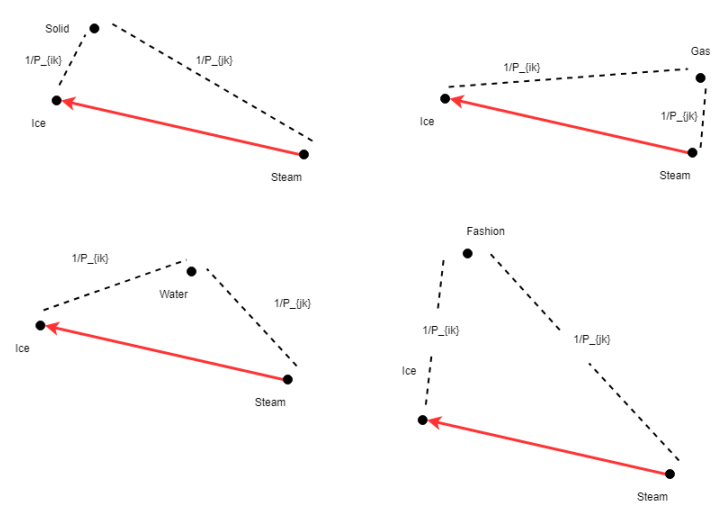
\includegraphics[width=0.95\textwidth]{img/g6.PNG}
    \caption{Behavior of vector distances with respect to $w_i - w_j$}
    \label{fig:g6}
\end{figure}

Then the authors introduced a transposition and a dot product as follows:
%To solve problem 2, the authors introduced a transposition and a dot product as follows:

\[
F((w_i - w_j)^\top u_k) = \frac{P_{ik}}{P_{jk}}
\]

They assumed that $F$ had an important property: homomorphism, so that they could write:

\[
F(w_i^\top u_k - w_j^\top u_k) = \frac{F(w_i^\top u_k)}{F(w_j^\top u_k)} = \frac{P_{ik}}{P_{jk}}
\]
\noindent
In other words, this homomorphism means that the subtraction $F(A-B)$ can be represented as a division $F(A)/F(B)$ and the two operations obtain the same result. And therefore,

\[
\frac{F(w_i^\top u_k)}{F(w_j^\top u_k)} = \frac{P_{ik}}{P_{jk}}
\]
\noindent
and, 

\[
F(w_i^\top u_k) = P_{ik}
\]
\noindent
The above relationship should be defined as:

\[
F(w_i^\top u_k) = c P_{ik}
\]
\noindent
for some constant $c$, considering that we cannot always assume that, given \\$F(A)/F(B) = G(A)/G(B)$, $F(A) = G(A)$ holds or that, given \\$F(A)/F(B) = 2F(A)/2F(B)$, $F(A) = 2F(A)$ holds. However in this case, if the similarity between $i$ and $k$ increases by a constant $c$, the similarity between $j$ and $k$ (for any $j$) will also increase by $c$. This means that all word vectors would be scaled by a factor $c$, which does not create a real problem and therefore the above can be assumed.

They set $F$ equal to the exponential function to enforce the property of homomorphism mentioned above: 

\[
\exp(w_i^\top u_k) = P_{ik} = \frac{X_{ik}}{X_i}
\]
\noindent
and therefore:

\[
w_i^\top u_k = \log X_{ik} - \log X_{i}
\]
\noindent
Since $X_i$ is independent of $k$ we can move it to the left:

\[
w_i^\top u_k + \log X_{i}= \log X_{ik}
\]
\noindent
Then they added some bias into the equation, we express $\log X_{i}$ as

\[
w_i^T u_k + bw_i + bu_k = \log(X_{ik}) 
\]
\[
w_i^T u_k + bw_i + bu_k - \log(X_{ik}) = 0
\]
\noindent
where $b_w$ and $b_u$ are network bias.

They observed that in an ideal environment, where you have perfect word vectors, the above expression would equal zero. Then they set the model's objective to minimize the following cost function:

\[
J(w_i, w_j) = (w_i^\top u_j + bw_i + bu_j - \log(X_{ij}))^2
\]

Then we come across a problem when $X_{ik} = 0$, which is the state when our cost function yields $\mathit{NaN}$, given that $log(0)$ is undefined. The GloVe authors proposed a smart solution: introducing a function $f(X_{ij})$ which weights words based on their frequency, in which infrequent words will have smaller weights. The \ac{GloVe} loss function is then:

\[
J = f(X_{ij})(w_i^\top u_j + bw_i + bu_j - \log(X_{ij}))^2
\]
\noindent
where $f(X_{ij})$ is defined as:

\[
f(X_{ij}) = 
\begin{cases}
(x/x_{\max})^a & \text{ if } x < x_{\max}\\ 
0 & \text{ otherwise}
\end{cases}.
\]

%Note that obtaining the co-occurrence matrix requires a single pass through the entire corpus to collect the required statistics. For a large corpus, this step can be computationally expensive, but it is a one-time cost upfront.

%\newpage


%\section{fastText}

%FastText is an extension of the word2vec architecture released by Facebook AI Research in 2016 [5]. FastText is %also an open-source library that allows users to learn text representations and text classifiers, available in %several languages.

%Instead of directly learning vectors for individual words, fastText represents each word as 
%an n-gram of characters. So, for example, if you take the word “artificial” with n = 3, the 
%fastText representation of this word is “ar, art, rti, tif, ifi, fic, ici, ial, al”. Once each word has 
%been represented using n-grams, we proceed as in word2vec: the neural network of the 
%word2vec model is trained to learn the embeddings and those of the corresponding matrix 
%are taken as word embeddings. Proceeding in this way, the authors highlighted how this 
%method allows embeddings to include suffixes and prefixes.


%FastText works well with rare words, without considering morphological inflection or other 
%lexical derivations (prefix or suffix): simply put, FastText aims to predict a category rather 
%than a word. Furthermore, this architecture features a hierarchical softmax.

%An important advantage of this method is that it can create word embeddings even for 
%words not seen in the training corpus. Indeed, if a word was not seen during training, it can 
%still be split into n-grams to obtain its embeddings. Both word2vec and GloVe, however, 
%do not provide any vector representation for words that are not in the dictionary of the model.

    %\chapter{State of the Art}
\label{chp:stateOfArt}

Geometrical representations of words are the building blocks in the field of \ac{NLP}, for higher-level tasks such as word sense disambiguation, sentiment analysis, and language modeling. The efforts for developing static word embeddings go all the way back to the 1980s, and currently there are many models in the literature each approaching the problem with a different methodology.

In this chapter, we will list and briefly describe some of the most known static word embedding models. This background will be later useful to demonstrate how our approach differs from others.

\section{Word2Vec}

One work that established a fundamental step in the field of \ac{NLP} is Word2Vec, which was presented in the article \cite{w2v} by Tomas Mikolov, Kai Chen, Greg Corrado, and Jeffrey Dean. More precisely, in this article, the authors present a shallow neural network-based training of two different architectures, namely, \ac{CBOW} and \ac{SG}.

\subsection{Skip-Gram}

We briefly describe the \ac{SGNS} embedding model introduced in \cite{w2v} trained using the negative-sampling procedure presented in \cite{w2v2}. 

\ac{SGNS} seeks to represent each word $w \in V_W$ and each context $c \in V_C$ as d-dimensional vectors $\overrightarrow{w}$ and $\overrightarrow{c}$, such that words that are “similar” to each other will have similar vector representations. It does so by trying to maximize a function of the product $\overrightarrow{w} \cdot \overrightarrow{c}$ for $(w, c)$ pairs that occur in $D$, and minimize it for negative examples: $(w, c_N)$ pairs that do not necessarily occur in $D$. The negative examples are created by stochastically corrupting observed $(w, c)$ pairs from $D$ - hence the name “negative sampling”. For each observation of $(w, c)$, SGNS draws $k$ contexts from the empirical unigram distribution $P_D(c) = \frac{\#(c)}{|D|}$. 



In the skip-gram model, each word $w \in W$ is associated with a vector $v_w \in \mathbb{R}_d$ and similarly, each context $c \in C$ is represented as a vector $v_c \in \mathbb{R}_d$, where $W$ is the words vocabulary, $C$ is the contexts vocabulary, and $d$ is the embedding dimensionality. The entries in the vectors are latent, and treated as parameters to be learned. Loosely speaking, we seek parameter values (that is, vector representations for both words and contexts) such that the dot product $v_w \cdot v_c$ associated with “good” word-context pairs is maximized.

More specifically, the negative-sampling objective assumes a dataset $D$ of observed $(w, c)$ pairs of words $w$ and the contexts $c$, which appeared in a large body of text. Consider a word-context pair $(w, c)$. Did this pair come from the data? We denote by $p(D = 1|w, c)$ the probability that $(w, c)$ came from the data, and by $p(D = 0|w, c) = 1 - p(D = 1|w, c)$ the probability that $(w, c)$ did not. The distribution is modeled as:


\[
p(D = 1|w, c) = \frac{1}{1+e^{-v_w \cdot v_c}}
\]

where $v_w$ and $v_c$ (each a $d$-dimensional vector) are
the model parameters to be learned. We seek to
maximize the log-probability of the observed pairs
belonging to the data, leading to the objective:

\[
{\arg\max}_{v_w,v_c} \sum_{(w,c) \in D}\log\frac{1}{1+e^{-v_c \cdot v_w}}
\]

This objective admits a trivial solution in which $p(D = 1|w, c)=1$ for every pair $(w, c)$. This can be easily achieved by setting $v_c = v_w$ and $v_c \cdot v_w = K$ for all $c$, $w$, where $K$ is large enough number.

In order to prevent the trivial solution, the objective is extended with $(w, c)$ pairs for which $p(D = 1|w, c)$ must be low, i.e. pairs that are not in the data, by generating the set $D'$ of random $(w, c)$ pairs (assuming they are all incorrect), yielding the negative-sampling training objective:

\[
{\arg\max}_{v_w,v_c} \left ( \prod_{(w,c) \in D}p(D=1|c,w)\prod_{(w,c) \in D'}p(D=0|c,w) \right )
\]

which can be rewritten as:

\[
{\arg\max}_{v_w,v_c} \left ( \sum_{(w,c) \in D} \log{\sigma(v_c \cdot v_w)}  \sum_{(w,c) \in D'} \log{\sigma(-v_c \cdot v_w)}  \right )
\]

where $\sigma(x)=1/(1+e^x)$. The objective is trained
in an online fashion using stochastic-gradient updates over the corpus $D \cap D'$.

The negative samples $D'$ can be constructed in various ways. We follow: for each $(w, c) \in D$ we construct $n$ samples $(w, c_1),...,(w, c_n)$, where $n$ is a hyperparameter and each $c_j$ is drawn according to its unigram distribution raised to the 3/4 power.

Optimizing this objective makes observed word-context pairs have similar embeddings while scattering unobserved pairs. Intuitively, words that appear in similar contexts should have similar embeddings.



    %!TEX root = ../main.tex

\chapter{Design of a New Model}
\label{chp:design}

In this chapter, we will introduce our static word embedding model by describing its background and architecture, and highlight its differences with respect to the state-of-the-art models in the literature.

\section{Preliminaries}
We will begin by establishing the fundamental symbols and concepts that will be employed throughout this chapter. 

\begin{itemize}
\item We consider the vector space $V = R^N$.
\item $T$ is a generic text used in the training process.
\item $u, v, w, u_1, . . .$ denote words appearing in $T$. Each individual word may have multiple occurrences in $T$, at different positions.
\item We use $p$, ${p}'$ to denote positions.
\item For a word $w$, $C(w)$ is the set of words appearing in $T$ in the context of $w$, that is, words that are found at some bounded distance from any occurrence of $w$ in $T$.
\item For each word $w$, $e_t(w)  \in V$ denotes a target vector embedding for $w$, and $e_c(w) \in V$ denotes a context vector embedding for $w$. 
\item $\tau$ is the target embedding matrix, and $\varsigma$ is the context embedding matrix.
\end{itemize}

Also, it will be useful to introduce beforehand some mathematical operations we will encounter later on.

\subsection{Sigmoid}
\label{sec:sigmoid}

The sigmoid function (or the logistic function) is a mathematical function that is used to map any real number to a value from the range defined between 0 and 1. When plotted, it has an S-shaped curve, which is the reason for its name. It is a popular and multipurpose function in the machine learning domain as it introduces non-linearity into models.

Sigmoid is a popular choice for making predictions in binary classification problems. It is a useful way of calculating the probability that an input belongs to one of the two classes. Sigmoid provides smooth transitions between the two extremes (0 and 1). In neural networks, the sigmoid function was historically used as an activation function in the hidden layers.

The sigmoid function is defined as:
\[ \sigma(x) = \frac{1}{1 + e^{-x}} \]

Where $x$ is the input, which can be any real number. Figure \ref{fig:sigmoid} visualizes the sigmoid function.

\begin{figure}[H]
    \centering
    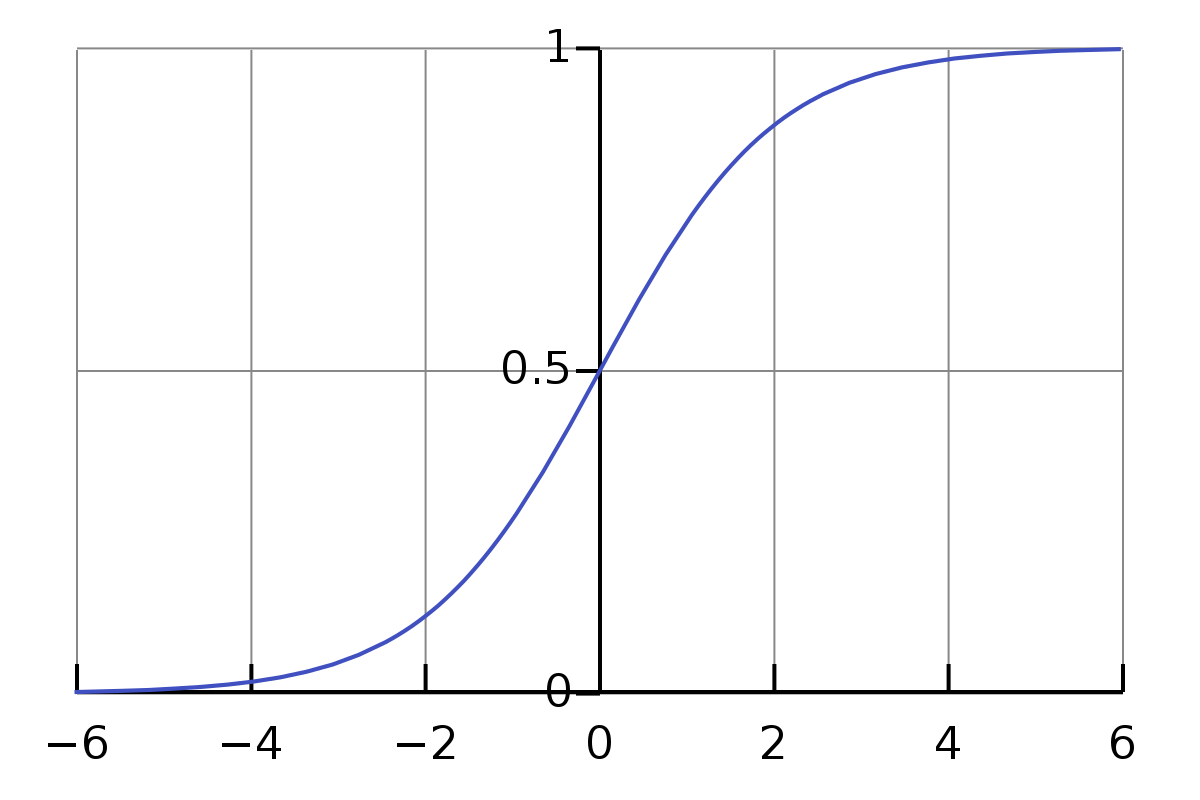
\includegraphics[width=0.6\textwidth]{img/sigmoid.png}
    \caption{Sigmoid function}
    \label{fig:sigmoid}
\end{figure}

We will use $\sigma$ for denoting the sigmoid function throughout this chapter.

\subsection{ReLU}

\ac{ReLU} is a widely used activation function in machine learning systems, especially in neural networks. \ac{ReLU} is a simple yet effective activation function that clamps negative values to zero and yields the input value as it is for non-negative inputs. It is computationally efficient, given that it is essentially a simple thresholding operation, making it faster to compute and more feasible for lower-end computing units. Thanks to its simplicity and non-linearity, it became the standard choice for many artificial neural networks.

The \ac{ReLU} function is defined as:
\[
\text{ReLU}(x) = \max(0, x)
\]
\noindent
where $x$ is the input, which can be any real number.


\subsection{Softplus}

Now we will present the softplus function, which is another mathematical function often used in machine learning. It is a smooth and differentiable unbounded function that maps any real number to a positive value.

The softplus function provides a smooth alternative to \ac{ReLU} and its variants (like Leaky-\ac{ReLU}). While \ac{ReLU} is a popular choice, especially as an activation function in deep neural networks, its behavior of mapping any non-positive value to zero might introduce problems in some settings. Readers are encouraged to have a look at \cite{softplus} for a better intuition for why the softplus function can be a better choice in some deep learning tasks, and why \ac{ReLU} is still a more popular option.

The softplus function ($\varsigma$) is defined as:

\[ \varsigma(x) = \ln(1 + e^x) \]
\noindent
where $x$ is the input, which can be any real number. In Figure \ref{fig:softplus}, we visualize the softplus function and compare it to the \ac{ReLU}.

\begin{figure}[H]
    \centering
    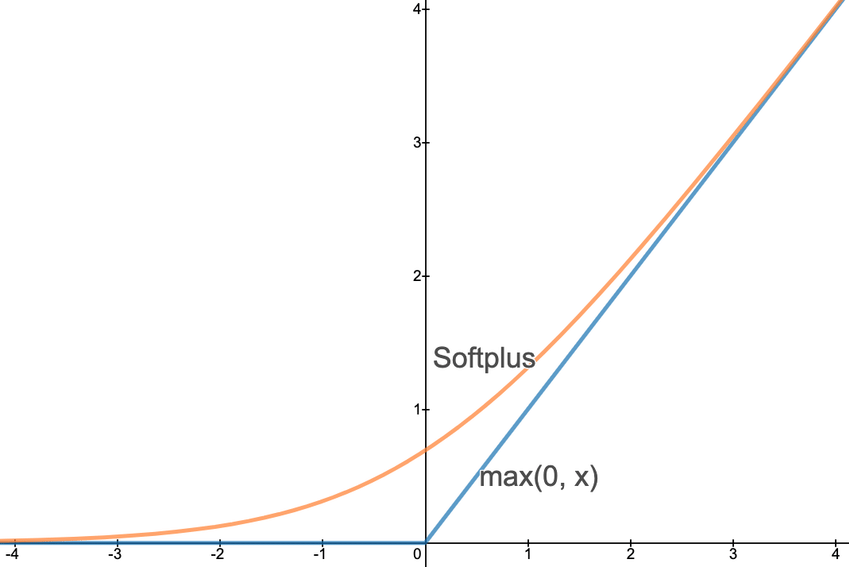
\includegraphics[width=0.6\textwidth]{img/softplus.PNG}
    \caption{Softplus function, compared to \ac{ReLU}}
    \label{fig:softplus}
\end{figure}

We will use $\varsigma$ for denoting the softplus function throughout this chapter.


\section{SGNS: Geometrical point of view}
Before sharing our idea of organizing embedding vectors in a vector space, it will be useful to first briefly introduce our understanding of the configuration learned by the \ac{SGNS} model. 

Let $w$ be a target word. The target of the \ac{SGNS} imposes that for every word $u \in C(w)$, $e_c(u)$ forms a “small” angle with $e_t(w)$.
This suggests the existence of an \textbf{N-dimensional cone} surrounding $e_t(w)$, and every $e_c(u)$ is contained in such cone. Coming from this, the model enforces words with similar contexts to have overlapping cones, hence the small angle between their target representations. This way, the model performs well in cosine similarity-based similarity tasks.

For describing this geometrical configuration based on the idea of context cones, a toy example in three dimensions may be useful. For this purpose, we prepared a figure visualizing how we expect the learning process to arrange context and target representations based on word occurrences. We imagine three target words: $w_1$, $w_2$ and $w_3$. For this example, imagine that $w_1$ and $w_2$ are two words that share similar contexts in $T$, whereas $w_3$ is not so related to the other two. Based on the training objective of \ac{SGNS}, we understand that we can expect to see a configuration similar to the one given in Figure \ref{fig:cones}.


\begin{figure}[ht]
    \centering
    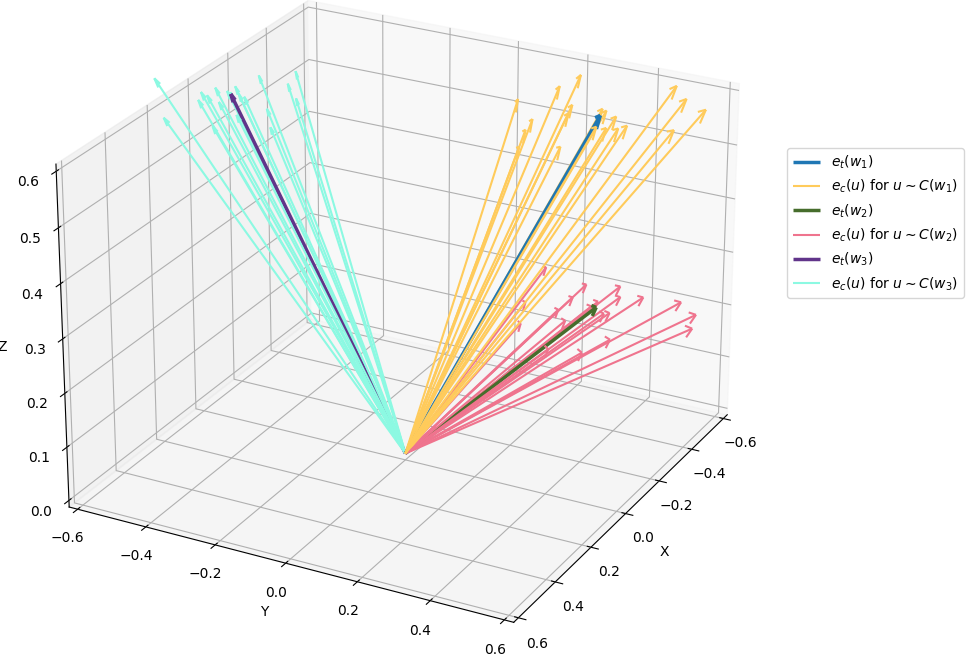
\includegraphics[width=0.9\textwidth]{img/context_cones.png}
    \caption{Context cones for three target words in three dimensions.}
    \label{fig:cones}
\end{figure}


In this figure, we highlighted the cone-like distribution of context word samples around the target word and the shared contexts of $w_1$ and $w_2$, hence the overlapping context cones. Thanks to this, it is easy to see that these two words will have greater cosine similarity than any other combination, and based on the distributional hypothesis, this is exactly what is desired. One should note that, however, this is just a visual prepared manually to assist the reader in following our intuition, and it will not be nearly as straightforward to observe similar shapes and distributions in a real training setting, given factors such as the high dimensionality, the size of the vocabulary and the noise.

Different models using different targets will yield either different geometrical configurations, or obtain similar results with different techniques. This is essentially what makes a model novel and the difference in the final configuration is what makes a model "better" in a task than some other model.

\section{Our model}
In this study, we propose a novel neural static word embedding model that is learned using orthogonal projections of vectors to represent contextual relationships. Many models, such as \ac{SGNS}, aim to capture contextual relationships of words based on one-to-one co-occurrences. Meanwhile, our model employs a third-order approach and leverages the contrastive learning paradigm, in which a positive training sample consists of a target word and two context words, and a negative sample consists of one target word, one context word, and a randomly sampled noise word from the corpus. This approach is distinct from the traditional static embedding models, and results in word embeddings that effectively capture contextual information in a higher-order, projective manner. 

We developed a unique geometrical loss function that aims to minimize the difference between the orthogonal projections of the selected context words onto the target word and maximize the difference between the orthogonal projections of the context word and the negative samples onto the target word.

We designed the training procedure using a neural network. Just like in \cite{w2v2}, we used two embedding matrices and we tuned these matrices as the weights of this feedforward network by backpropagating the gradients of our loss function.

\section{Design choices}

In developing our model and designing the training pipeline, we needed to make certain choices, and each decision needed to be carefully analyzed in order to maximize the performance of the final model. Some of these decisions needed to rely on other works, but some of them needed to be tested out for our specific needs.

\subsubsection{Number of embedding matrices}

We first investigated whether or not it is logical to use two embedding matrices, just like how they proposed in word2vec \cite{w2v2}. They use two representations for each word $w$, $e_t(w)$ and $e_c(w)$. $e_t(w)$ is the target embedding of $w$ which is the final product, and $e_c(w)$ is the context embedding, which is only used during the training. We have trained an \ac{SGNS} model with an implementation found online, using both single-embedding and two-embedding approaches. The results indicated the benefit of two embeddings. We were convinced that the same would apply to our model as well since both models leverage the contrastive learning paradigm.

%\subsubsection{Embedding dimensions} % Move this section

%The embedding dimension is yet another thing that directly influences the final performance. It is the factor that sets the amount of information that can be stored in an embedding vector. Based on this, we found that the dimension of 300 is quite a common choice in the literature, and it is a good number for our memory and processing resources.

\subsubsection{Negative samples} 

Our model's loss function works on both negative and positive samples, this means for a target word $w$, we need its context words $C(w)$ for positive training samples. On the other hand, $C(w)$ and $w_n$ are needed for a negative training sample, where $w_n$ is a noise word randomly sampled from the training corpus. \cite{w2v2} uses a factor $k$ which is the number of negative training samples for each positive training sample. It is the common practice to keep this number greater than one. 

As for the sampling of the $w_n$ for each negative training sample, the natural idea would be picking a random word from the vocabulary, following a uniform probability distribution. But we again decided to follow the findings reported in \cite{w2v2} and work with a sampling table. In this technique, based on the word occurrence frequencies, we generate a sampling table and we pick a $w_n$ from this table at random. A word appears on this table many times which is proportional to its frequency, which can be expressed as follows: 

\[m_w = \frac{f_w^{0.75}}{Z}\]
\noindent
where $m_w$ is the number of times a word occurs on this sampling table, $f_w$ is the number of occurrences of this word in the vocabulary, and $Z$ is computed as follows:

\[Z = \sum_{w}^{V} f_w^{0.75}\]

\subsubsection{Positive samples}

For generating training samples, we needed to obtain the contexts of each target word. The context of a word occurrence is the set of words that appear at a limited distance from that target word occurrence. For this purpose, one needs to set a parameter $L$, which is the size of the context window. The context is collected for a target occurrence from the $L$ distance on the left and right of the target word. For instance, for a fixed window implementation, let us fix the parameter $L$ to 2 and target $w$ as "\textit{web}". In the following sentence:

\begin{displayquote}
Many desktop publishing packages and \underline{web} page editors now use Lorem Ipsum as their default model text.
\end{displayquote}

If we use a string preprocessing to eliminate conjunction, $C(w)$ consists of: "\textit{publishing, packages, page, editors}". These are the words that we can easily associate with the meaning we derive from the word "\textit{web}". If we change our mind and set $L=4$, now $C(w)$ consists of: "\textit{many, desktop, publishing, packages, page, editors, now, use}". Even though we can still associate these words with "\textit{web}", it is easy to see that as we extend the window size, we will come across words that are less strictly related to our target word. This might introduce noise to our learning but also enable us to learn more far-sighted relations of words. Coming from this, we needed to be mindful while choosing the window size, as it would directly influence the relations of the word representations.

What we described above links with an approach called "\textit{Fixed-Sized Context Window}". We combine this with another approach, "\textit{Dynamic Context Windows}", to add a bit of randomness to it.

Dynamic context windows approach is a way of leveraging the advantages of multiple window sizes throughout the training. Based on some factor, or completely at random, one can keep changing the size of a context for each training sample. We decided to follow this approach and picked the window size from $[2, L+1]$ for each sample at random. By keeping this dynamic range dependent on the pre-defined parameter $L$, we keep control of more or less how many words are to be collected on average from each context window, but still leveraging from the randomness that comes from the dynamic approach.

\section{3rd order loss}
\label{sec:loss}

For any machine learning model, the loss function is the main factor that determines the characteristics and the purpose of the model by setting the objective. Word embedding models are no exception, depending on the loss function used, the embedding models can be enabled to capture complicated contextual relationships of words with increasing accuracy, in order to succeed in downstream tasks.

When we decided to work with a third-order structure, our objective was capturing contextual relationships in a higher order, with the aim of obtaining vectors encoding more complex relationships than what can be captured with traditional models. 

Throughout our study, we continuously made changes to our loss function and reported the results. In this section, we will talk about our "base" model, which was our starting point when we implemented a new loss function. More about the specifications of our base model and how its variants differ from it will be explained in Chapter \ref{chp:experiments}.

\begin{figure}[ht]
    \centering
    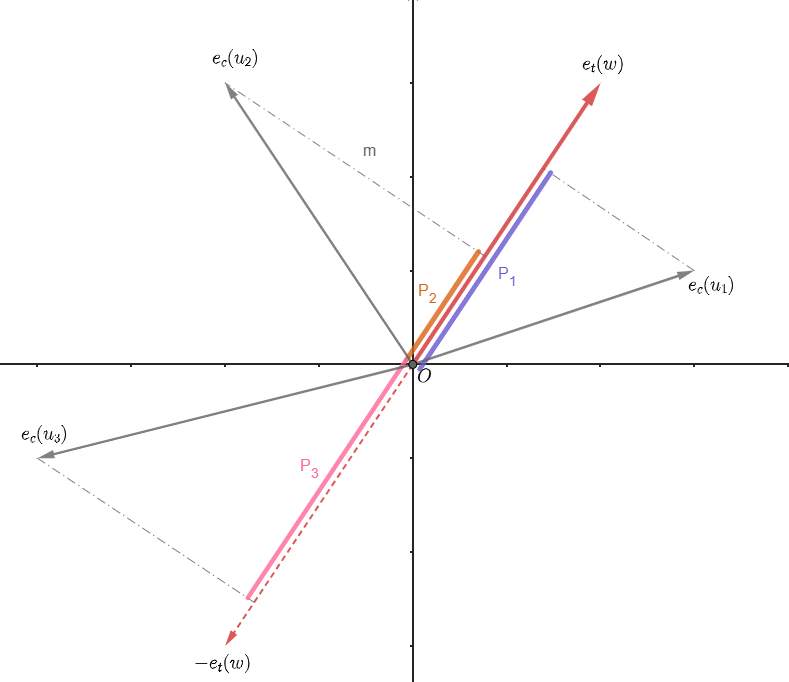
\includegraphics[width=0.8\textwidth]{img/loss_plot.png}
    \caption{One target and three context embedding vectors, and orthogonal projections onto the target vector.}
    \label{fig:loss_plot}
\end{figure}

Let us describe the objective of our training using Figure \ref{fig:loss_plot}. Here, we see four vectors for four words, $w, u_1, u_2, u_3$. $w$ is our target word, we show its target embedding vector. The rest are other words sampled from the vocabulary, and we see their context representations. As we said earlier, our loss function is based on orthogonal projections, therefore we also show the orthogonal projections of these context representations onto the target representation of $w$, $e_t(w)$.

Dotted lines connecting context vectors to the target vector visualize the projections. Colored lines show the magnitude of the orthogonal projections. $P_1, P_2, P_3$ visualize the magnitudes of the orthogonal projections of $u_1, u_2 , u_3$ respectively, onto the target representation of $w$.

Our loss function has two components. Let us imagine training samples, using the vectors in Figure \ref{fig:loss_plot}. One positive sample, $(w, u_1, u_2)$, consists of a target word and two context words sampled from the context window of one occurrence of the target word. And one negative sample, $(w, u_1, u_3)$, consisting of one target word, one context word, and a noise word sampled from the vocabulary. Using these, the components of the loss function are:

\begin{itemize}
\item \textbf{Positive Loss $\myscore{+}{w, u_1, u_2}$:} Forces context words $u_1$ and $u_2$ to have similar projections onto the target $w$. Uses positive training samples. Penalizes the projection difference of the context embeddings of two context words, $e_c(u_1)$ and $e_c(u_2)$ onto the target representation of the target word, $e_t(w)$. In other words, aims to minimize $| P_1 - P_2 |$.
\item \textbf{Negative Loss $\myscore{-}{w, u_1, u_3}$:} Uses negative training samples. Aims to push the noise projection to the left side of the context projection, onto the target vector. In order words, aims to maximize $P_1 - P_3$.
\end{itemize} 

Overall loss $L$ is calculated for our two training samples as:

\[L = - \left ( \log{\myscore{+}{w, u_1, u_2}} + \log{\myscore{-}{w, u_1, u_3}} \right )\]
\noindent
We use $\log$ for a more efficient convergence since both positive and negative loss yield small values. Generalizing this formula for every training sample generated for each word in the vocabulary:

\[L = - \sum_{w \in V} \left (\sum_{u_1, u_2 \in C(w)} \log{\myscore{+}{w, u_1, u_2}} + \sum_{u_1 \in C(w), u_3 \sim S, u_3 \notin C(w)} \log{\myscore{-}{w, u_1, u_3}}\right )\]

Where $S$ is our negative sampling table.

\subsection{Positive loss}

Now we will have a closer look at the computation of the positive loss, $\myscore{+}{w, u_1, u_2}$. We will continue using our example positive training sample $(w, u_1, u_2)$ from Figure \ref{fig:loss_plot} in our descriptions.

As we discussed earlier, this part of our loss aims to minimize the projection difference of context representations of the context words onto the target representation of the target word. In other words, our goal is to minimize $| D = P_1 - P_2 |$. $D$ is calculated as follows:

\[ D = \frac{e_c(u_1) \cdot e_t(w) - e_c(u_2) \cdot e_t(w)}{\left \| e_t(w) \right \|}\]

Using $D$, the calculation of $\myscore{+}{w, u_1, u_2}$ is:

\[ 
\myscore{+}{w, u_1, u_2} = 2 \cdot (\sigma( \varsigma  (D) ))
\]
\noindent
where $\sigma$ is the sigmoid function and $\varsigma$ is the softplus function.

By applying the softplus function to $D$, we first ensure that $P_1 - P_2$ is positive. It will fix the negative values to a positive value near zero. We went with softplus instead of \ac{ReLU}, because softplus is continuous and differentiable everywhere unlike \ac{ReLU}, and almost as resource-efficient. Nevertheless, we still tested this decision by employing \ac{ReLU} in another version of our model (see Section \ref{sec:variants}), and the results proved the superiority of softplus. Not learning from the samples where $D$ is a negative value might seem like a loss of information, however, we should note that the existence of a positive sample $(w, u_1, u_2)$ ensures the existence of another positive sample $(w, u_2, u_1)$ thanks to our implementation of the sampling procedure.

Next, this value is passed through a sigmoid operation, and this yields a probability. Then, it is multiplied by two, so that the impact of the positive loss is amplified. We decided this was needed because the negative loss was dominating the positive loss, considering that the negative loss is calculated for five samples per one positive sample.

\subsection{Negative loss}
\label{sec:neg_loss}

Next, we describe the computation of the negative loss, $\myscore{-}{w, u_1, u_3}$. We are still proceeding with our example negative training sample $(w, u_1, u_3)$ from Figure \ref{fig:loss_plot}.

This part of our loss aims to maximize the projection difference of context representations of the context words and the context representation of the noise samples, onto the target representation of the target word. In other words, our goal is to maximize $D = P_1 - P_3$. $D$ is calculated as follows:


\[ D = \frac{e_c(u_1) \cdot e_t(w) - e_c(u_3) \cdot e_t(w)}{\left \| e_t(w) \right \|}\]

Then using $D$,

\[ \myscore{-}{w, u_1, u_3} = 2 \cdot (\sigma( \varsigma  (D) )) - 1\]
\noindent
Again, $\sigma$ is the sigmoid function, and $\varsigma$ is the softplus function.

By designing a loss function that combines the negative and positive loss as we described, we aim for context word projections to be similar and for negative word projections to be distinguished from them. We make this distinction by pushing the noise word projections to the left along the target word vector. Note that by employing a random initialization, initially, we have all projections distributed randomly around $0$. Coming from this, it is straightforward to see that we encourage context projections to align on the positive side, while noise projections will be pushed to have negative values.

\section{The predecessor model}

When we started working on this word embedding model, we leveraged the findings provided in an earlier study. This study was a Master's dissertation which was completed by Elena Galvan, under the supervision of Prof. Giorgio Satta, submitted in 2022 \cite{galvan}. This study was another attempt to produce a word embedding model in the third order, using similarly structured positive and negative loss functions. Their approach is similar to ours in a lot of ways but also has major differences in terms of implementation, evaluation methods, loss calculations, and data analysis. That study provided us with a good starting point, but the model produced was not performing as expected. Therefore we aimed to find what was not working in that design, conduct experiments to understand the model behavior, and further improve it to achieve the best possible performance.



\section{Our model: Geometrical point of view}

When we designed and constructed this model, we were inspired by some geometrical idea of a uniquely organized word embedding vector space, and every decision we made for this system was made to achieve this organization. In this section, we will talk about the organization we hoped to achieve and the reasoning behind it.

Let $w$ be a target word. We create positive training samples using the words collected from a fixed distance for each occurrence of $w$ in $T$. As enforced by $\myscore{+}{w, u_1, u_2}$, we desire that each word sampled from the same context of $w$ must have equal or similar orthogonal projections onto the target representation of $w$. In contrast, each noise word sampled to pair with a context word to form a negative training sample is forced by $\myscore{-}{w, u_1, u_3}$ to have a smaller projection onto the target compared to the context projections. In other words, $\myscore{+}{w, u_1, u_2}$ enforces similar context words to be grouped together, while $\myscore{-}{w, u_1, u_3}$ enforces noise words to be cleared from them by their projections being pushed to the left side along the target vector.

We need to highlight that when we create samples, we combine the context words only with the other words in the same context. For example, except for some unexpected occurrences, if the target word is "bat", we usually expect to encounter positive samples containing context pairs such as \textit{(rabies, caves)}, \textit{(mammal, blind)}, or \textit{(fly, sleep)}. Other times, we can also encounter pairs like \textit{(baseball, ball)}, \textit{(hit, base)}, or \textit{(pitcher, helmet}). However, our implementation is not designed to mix these distinct word senses up, therefore we do not expect to sample context pairs such as \textit{(animal, glove)}, \textit{(batman, teams)}, or \textit{(major, pregnancy)}.

Thanks to this property, we expect our model to yield word embeddings such that when we look closely at the context embeddings, we are expecting to find different contexts of a given target word to have grouped orthogonal projections. This does not mean a small Euclidean distance to the target word nor a small angle in between. Going back to our "bat" example, we are expecting the context representations of words like \textit{rabies, caves, mammal, blind} to have similar projections onto the target representation of the word "bat". Meanwhile, we expect to find the same for the words like \textit{baseball, ball, hit, base}, but on some different range than the context words belonging to the animal sense of the word "bat".

As for the negative loss, we expect $\myscore{-}{w, u_1, u_3}$ to enforce noise word projections to be pushed to the left side of these groupings along the target vector. This way, the groupings stacked next to each other along the target vector will have minimal noise around and it will be much easier to distinguish them.

Ideally, we expect these "groupings" to form \textbf{context hyperplanes} in $N-1$ dimensions, when the embeddings are defined in dimension $N$. In other words, we expect a target word representation of a word $w$ to be orthogonal to a set of hyperplanes, each representing a different sense or context of $w$. From this, we imagine different words in the vocabulary sharing similar contexts to be orthogonal to similar hyperplanes, i.e. hyperplanes sharing a large volume of context words. This way, they can form high angular similarities in between. Also, with the impact of $\myscore{-}{w, u_1, u_3}$, we ensure that other words in the vocabulary with less similar contexts are orthogonal to hyperplanes elsewhere, discouraged from forming small angles with dissimilar words.

Let us revisit the Figure \ref{fig:loss_plot}. If we take a negative sample $(w, u_1, u_3)$, it is easy to see that the projection difference, $D = P1 - P3$, is maximized. Consequently, if some other word $w_2$ has the word $u_3$ in its context windows frequently but $u_1$ not so much, $e_t(w_2)$ is encouraged to form a large angle with the vector $e_t(w)$, therefore the cosine similarity will be small, which is exactly what is desired by the similarity tasks.


    %!TEX root = ../main.tex

\chapter{Implementation}
\label{chp:implementation}

In this chapter, we will get into the implementation techniques and tricks we employed for the training of our word embedding model. While the theory and design are critical, this is yet another aspect of our work that directly influences the outcome. We will explain the software techniques we used and the reasoning behind our decisions. We will also demonstrate how we implement these ideas in our code. By understanding what we have done to achieve what, the reader will have a better idea about how to reason the strengths and the shortcomings of our model, and what can be done to improve it. We will stick to the notation introduced in the previous chapter when it is needed.

\section{Setup}

We implemented our training and other experiments using Python version 3.10.12, which is one of the most recent versions at the time of this dissertation. Python is a popular choice for projects involving machine learning for reasons such as:
\begin{itemize}
    \item \textbf{Ecosystem}: A wide range of libraries and frameworks that are specifically designed for \ac{NLP} and \ac{ML} tasks. Libraries like \ac{NLTK}, PyTorch, scikit-learn, and TensorFlow provide a wealth of tools for these projects.
    \item \textbf{Ease of Use}: Python is easy to learn and use. Compared to more traditional, lower-level programming languages, it greatly reduces the amount of code required for different tasks. It is known for its elegant and easy-to-read syntax that makes it accessible and easy to collaborate on.
    \item \textbf{Vast Community}: Python has a large and active user community, consisting of professionals from a wide range of domains. One can easily find solutions to even very specific problems and access documentation.
    \item \textbf{Data Manipulation}: There are numerous data manipulation and analysis tools available in Python, which is the backbone of the majority of the \ac{ML} projects. Libraries like NumPy and pandas are common choices for handling and processing large datasets, making it possible to shape the data to the desired format and easily capture interesting properties of the data samples in hand.
\end{itemize}

We practiced cloud computing for this project and used Google Colab as our development environment. Google Colab offers free but limited use of GPU computations. Their free plan grants access to NVIDIA T4 GPU, but for a monthly fee users can also use NVIDIA A100 and V100 paired with a higher memory. Since the computational resources are better and the timeouts are reduced in the paid plan, we subscribed to their paid plan for this study. Google Colab offered several key advantages, including:

\begin{itemize}
    \item \textbf{Portability}: We were able to run our programs from any device connected to the internet, without the need for any installations.
    \item \textbf{Integration with Google Drive}: We stored our files like our logs, datasets, and models on Google Drive, which makes everything more organized and accessible from anywhere in the world.
    \item \textbf{Ease of Collaboration}: Notebooks are quite easy to share, a link can grant access to anyone for viewing or manipulating our experiments, with no downloads or system requirements.
    \item \textbf{Interactivity}: We were able to visualize and modify our code in real-time, which makes it possible to detect and fix errors early on, and rapidly add new ideas to our code.
    \item \textbf{Version Control}: Colab keeps track of the versions of a notebook, making it easier to track changes and go back to an earlier version if needed.
\end{itemize}

We utilized a variety of libraries in our training procedure, but the backbone of our training procedure was built using PyTorch. PyTorch served as the cornerstone of our project, enabling us to define our model architecture and facilitating the crucial process of learning. It not only provided us with a blueprint for our objects but also was crucial for utilizing GPU resources for our multi-dimensional computations. By harnessing the power of PyTorch for machine learning and GPU utilization, NumPy for efficient numerical operations, and Matplotlib for creating visualizations, we successfully crafted, trained, and closely monitored our model's progress and performance.


\section{Preprocessing}
\label{sec:preprocessing}

It is common practice to apply a multi-step preprocessing procedure to the corpus. What we do in this step of our implementation is often called \textit{text normalization}. Text normalization is the process of transforming text-formatted data into a pre-defined form by applying a set of operations in an order. It is crucial to do so for several reasons. For one, just like any other machine learning task, one needs to reformat the data so that the machine learning model can process it. Secondly, a good preprocessing of the training data can greatly enhance the performance of the final product.

Generally, text normalization involves a combination of several tasks. Even though there are general blueprints for specific needs and a catalog of tasks to pick from, the choice greatly depends on the structure of the data and the task at hand. Some of the common tasks include spell checking, contraction, handling punctuation, tokenization, case folding, stop word removal, and stemming. Without going into the details of other possible tasks we could have applied to our data, we will talk about our own procedure.

We are not aiming to produce a case-sensitive model, therefore we start by lower-casing our entire corpus. This way, every occurrence of a type is equalized. This process is also called \textit{case folding}. Even though this is a popular choice for the normalization process, it comes with its downsides. For example, when we lowercase everything, our model will not be able to distinguish some entities such as "cologne", a liquid with a pleasant smell, and "Cologne", a city in Germany. However, we still go for it, considering that it will enable us to utilize our data better in every other case.

\begin{lstlisting}[language=Python, caption=Case folding]
text = text.lower()
\end{lstlisting}

Next, we handle punctuation. We handled punctuation symbols rather than removing them because our belief was that punctuation influences the meanings of linguistic expressions greatly, therefore they are important for lexical meanings as well, especially for a third-order model like ours. By handling punctuation, we mean replacing their occurrences with identifiers.

\begin{lstlisting}[language=Python, caption=Handling Punctuation]
text = text.replace('.', ' <PERIOD> ')
text = text.replace(',', ' <COMMA> ')
text = text.replace('"', ' <QUOTATION_MARK> ')
text = text.replace(';', ' <SEMICOLON> ')
text = text.replace('!', ' <EXCLAMATION_MARK> ')
text = text.replace('?', ' <QUESTION_MARK> ')
text = text.replace('(', ' <LEFT_PAREN> ')
text = text.replace(')', ' <RIGHT_PAREN> ')
text = text.replace('--', ' <HYPHENS> ')
text = text.replace('\n', ' <NEW_LINE> ')
text = text.replace(':', ' <COLON> ')
\end{lstlisting}

Now that we have our corpus lower-cased and punctuation handled, we are ready to turn this text-formatted data into a list of words. This process is a type of tokenization, called \textit{word tokenization}. We are interested only in words themselves, but other tokenization techniques, such as \textit{sub-word tokenization}, can be employed when one is interested in training a model that can represent lower-level expressions and form embeddings for previously unseen words using this finer-grained knowledge. For applying word tokenization, we simply split our text from white-space characters.

\begin{lstlisting}[language=Python, caption=Word Tokenization]
words = text.split()
\end{lstlisting}

Next, we apply word frequency filtering, which means we remove the words from our data that have less or equal to a predefined number of occurrences. This number is a parameter that the designers can choose, we went with a popular choice, which is five. This will lower the variety of words we will learn during the training, but it will enable us to learn better relationships among "more important" words by reducing the size of our vocabulary.

\begin{lstlisting}[language=Python, caption=Word Frequency Filtering]
word_counts = Counter(words)
trimmed_words = [word for word in words if word_counts[word] > 5]
\end{lstlisting}

Then we remove some words that we believe do not carry useful information. The scale of this removal can vary based on the choice of the designer. But considering we already suffered from long training times and we have been training our model over and over again for exploration, we decided to go for a very aggressive one. This might cause our model to miss out on some words that may be very important for some specific contexts, but it increases our training efficiency and enables us to reduce the noise to learn better about more important words in our corpus.

\begin{lstlisting}[language=Python, caption=Stopword Removal]
stop = [
  "a", "about", "above", "after", "again", "against", "all", "also", "altough", "am", "an", "and", "any", "are", "aren't", "as", "at", "b", "be", "because", "been", "before", "being", "below", "between", "both", "but", "by", "c", "can", "can't", "cannot", "could", "couldn't", "d", "de", "did", "didn't", "do", "does", "doesn't", "doing", "don't", "down", "during", "e", "each", "either", "even", "f", "few", "for", "from", "further", "g", "h", "had", "hadn't", "has", "hasn't", "have", "haven't", "having", "he", "he'd", "he'll", "he's", "her", "here", "here's", "hers", "herself", "him", "himself", "his", "how", "how's", "however", "i", "i'd", "i'll", "i'm", "i've", "if", "ii", "in", "into", "is", "isn't", "it", "it's", "its", "itself", "j", "just", "k", "l", "like", "m", "many", "may", "me", "more", "most", "much", "must", "my", "myself", "n", "nd", "neither", "no", "nor", "not", "now", "o", "of", "off", "on", "once", "only", "or", "other", "our", "ours", "ourselves", "out", "over", "own", "p", "q", "r", "rd", "s", "same", "shall", "she", "she'd", "she'll", "she's", "should", "shouldn't", "so", "some", "such", "t", "th", "than", "that", "that's", "the", "their", "theirs", "them", "themselves", "then", "there", "there's", "these", "they", "they'd", "they'll", "they're", "they've", "this", "those", "though", "through", "to", "too", "u", "under", "until", "up", "us", "v", "very", "w", "was", "wasn't", "we", "we'd", "we'll", "we're", "we've", "were", "weren't", "what", "what's", "when", "when's", "where", "where's", "which", "while", "who", "who's", "whom", "why", "why's", "will", "with", "won't", "would", "wouldn't", "x", "y", "you", "you'd", "you'll", "you're", "you've", "your", "yours", "yourself", "yourselves", "z", "zero", "one", "two", "three", "four", "five", "six", "seven", "eight", "nine", "ten", "eleven", "twelve"
  ]

stop_trimmed_words = [w for w in trimmed_words if w not in stop]
\end{lstlisting}


\section{Subsampling}
\label{sec:subsampling}

The process of subsampling involves eliminating some of the occurrences of some words through a probability distribution. This probability distribution is created in a way that words with a lot of occurrences are more likely to lose some of their occurrences. We see this process is applied usually to get rid of the stopwords, but that is something we have already done in the preprocessing step. Nevertheless, we decided that balancing out the word occurrences will benefit our learning process, and also improve the training efficiency.

The aforementioned probability distribution is based on the word frequencies. For a word $w_i$, the probability of removal of each of its occurrences, $P(w_i)$, calculated as:


\[
P(w_i) = 1 - \sqrt{\frac{t}{f(w_i)}}
\]
\noindent
where $t$ is the subsample threshold that should be set by the designers based on the corpus size, and $f(w_i)$ is the number of occurrences of the word $w_i$.

We used the subsample threshold as $1e-5$.


\begin{lstlisting}[language=Python, caption=Subsampling]
freqs = {word: count / len(int_words) for word, count in word_counts.items()} 
# Yields a dictionary: (word index) : (normalized frequency)
p_drop = {word: 1 - np.sqrt(subsample_threshold / freqs[word]) for word in word_counts} 
# Yields a dictionary: (word index) : (P(w_i))

train_words = [word for word in int_words if random.random() < (1 - p_drop[word])] 
# List of words after subsampling

\end{lstlisting}


\section{Low context removal}
\label{sec:lowcontext}

In our code, we have tested out one more process to downsize our vocabulary. This time, we considered for each word $w_i$, the size of $C(w_i)$ for all occurrences of $w_i$ in the entire corpus. 

Our belief was that given the dimension of our representations, we simply do not have enough information to learn from if a word does not have enough context. Therefore it simply becomes "noise" in the vector space. Moreover, when we analyzed the sizes of the contexts for each type, we found that the majority of the words do not go above a certain threshold, leaving the impression that they are underrepresented. Figure \ref{fig:context_pie} shows the ratios of context sizes of words in our vocabulary, after the preprocessing and subsampling. These numbers are calculated for randomized context windows for $L$ ranging between $2$ and $6$.

\begin{figure}[ht]
    \centering
    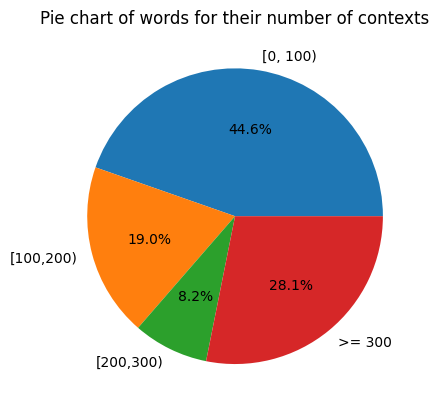
\includegraphics[width=0.7\textwidth]{img/context_pie.png}
    \caption{Number of context words of words in our vocabulary.}
    \label{fig:context_pie}
\end{figure}

When this is the case, removing the underrepresented words from our vocabulary would greatly downsize our training data, but possibly facilitate a better learning for the remaining of the words.

The process of low-context removal starts with counting the number of context tokens surrounding the given word in the text for the given window size. If we find that this number is smaller than the predefined threshold, this type will be eliminated from our train data entirely.

After our testing, we figured there was no real advantage introduced by this process, in contrast, we observed a big performance drop in our final model. Therefore this process is removed from the training pipeline in our base model.

\section{Training and validation split}
\label{sec:val_split}

In the earliest versions of our models, we simply used the entire corpus for the learning, then we evaluated our models on similarity and relatedness tasks. After a while, we decided to partition our corpus into two sets, one for validation and one for learning. 

A validation set is useful for monitoring if our model is still learning meaningful patterns from the data, or is just simply starting to memorize it. After all, we are trying to capture contextual relationships of words, not training a model that perfectly fits our selected training corpus. Removing a portion from our training set for some other purpose will decrease the amount of information to learn from, but we concluded that the advantages of this practice are worth the loss of information.

We decided to use $10\%$ of our corpus for the validation. Given that we are already working with a relatively small corpus, we believe that this portion will not affect our learning greatly, but we still have enough data for a fair validation. We also made sure that the validation set does not include words that are not introduced to our model by the training data. The way we make sure of this can be found in Code \ref{code:val_partition}, starting from line number $6$.

\begin{lstlisting}[language=Python, caption=Training and Validation Set Split, label={code:val_partition}]
# Train - Validation split
split_index = int(len(train_words) * val_partition)
validation_words = train_words[:split_index]
train_words = train_words[split_index:]

# Validation set should not introduce new types
exclude_from_val = set(validation_words) - set(train_words)
validation_words = [w for w in validation_words if w not in exclude_from_val]

\end{lstlisting}

We will show how we perform our validation later in this chapter.

It should be noted that in the majority of machine learning training procedures, it is a useful practice to employ \textit{K-Fold Cross Validation}, in order to leverage the advantages of use of a validation set, by also minimizing the cost of reducing the amount of data to learn from. However, this procedure is also rather time-consuming. Since we are dealing with time and computational power limitations, and we are more interested in observing what our model can possibly promise, we leave this technique as a future improvement.

We should note that we did not partition a test set, since we are not really interested in the loss obtained from another piece of text anyway. Our focus in this study is to learn a set of embeddings, that can perform well on and compete against state-of-the-art models in tasks such as similarity, relatedness, or analogy.

\section{Training loop}

Now we proceed to the learning phase. We use Adam optimizer and our custom model and the loss for the training. In some other variants of our base model, we also tested learning rate decay, however for the base model we set the decay rate to $1.0$, which means it is left unchanged.

Throughout the training, we did our best to keep track of everything and save the models that could be useful for our experiments later. We printed out the training and validation loss in regular intervals, and once the learning was concluded we visualized our logs.

The training loop is a nested \verb|for| loop. The outer loop iterates for the number of epochs. We usually ran six epochs, which seems to be even more than enough in some settings. The inner loop iterates over the training batches, which includes positive and negative training samples that are explained in the previous chapter. In each step, first, we calculate loss, backpropagate it, and in some steps, print out the results. After each epoch, we calculate the loss on our validation set. This gives a better idea about our progress achieved in the last epoch. 

Each time we calculate the training or the validation loss, we compare the performance to the best one we encountered up to that time step. If it is the best one we have seen, we save the model for later use. We also save every model we obtain at the end of each epoch.

\section{Context and noise sampling}

Given a target word $w$, for calculating $\myscore{+}{w, u_1, u_2}$ and $\myscore{-}{w, u_1, u_3}$, we need to sample context words from $C(w)$ and noise words from the negative sampling table. 

Let us have a refresher about the training samples we use. A positive training sample is $(w, u_1, u_2)$, where $u_1$ and $u_2$ are different tokens sampled from $C(w)$. A negative training sample is $(w, u_1, u_3)$, where $u_1$ is again sampled from $C(w)$ and $u_3$ is a noise word sampled from the sampling table.

Our training samples are provided in batches by a generator function which we iterate on in our training loop. It takes as input the training set, batch size, context window size ($L$), the number of negative training samples for each positive training sample, and a dictionary that maps a word index to the list of its context words. The last one is only used when low-context removal is enabled.

\begin{lstlisting}[language=Python, caption=Batch generating function - Part 1]
def get_batches(words, batch_size, win_size, neg_samp, idx_to_contexts):

  n_batches = len(words) // batch_size # Number of batches
  words = words[:n_batches * batch_size] # Keep only the number of words to match the bath_size and n_batches

\end{lstlisting}

Then we iterate over the training set with a step size equal to the batch size. At each step of this loop, we generate the positive and the negative training samples and yield one training batch. It starts with creating an empty list for the target word, two lists for context words, and lists used for sampling each sample. The list of the noise words will be created later. 

This generator yields 4 lists, one containing target words, two containing context words, and one containing noise words. The list containing noise words is two-dimensional, and its second dimension is equal to the number of negative samples to be generated per each positive sample (factor $k$).

\begin{lstlisting}[language=Python, caption=Batch generating function - Part 2]
  for idx in range(0, len(words), batch_size): # for each batch in words
    central_words = []  # list containing target words
    context_words1 = []  # list of words in the context, second order
    context_words2 = []  # list of words in the context, third order

    x, y = [], [] # lists that store the target and context words for each training sample
    z = [] # list of tuples that stores the starting and ending indices of each training sample in the x and y lists
    a = 0 # Counter for the total number of training samples seen so far. Used to keep track of the indices in z.
\end{lstlisting}

A training sample is obtained by using the same index in the lists that are generated by this function. In other words, elements corresponding to the same index in each of these lists are used to generate training samples. For example, using an integer $i$, one positive sample is (\verb|central_words[i]|, \verb|context_words1[i]|, \verb|context_words2[i]|). % \verb|central_words|

Next, we go into an inner loop. This time, we iterate for \verb|batch_size| number of target words and generate positive and negative samples for them.

\begin{lstlisting}[language=Python, caption=Batch generating function - Part 3]
    batch = words[idx:idx + batch_size] # one batch; batch_size number of words (unique), starting from index idx

    for ii in range(len(batch)): # in a batch
      batch_x = batch[ii] # target word for a given training sample
      batch_y = get_context(batch, ii, win_size, idx_to_contexts) # list of context words for that target word

      y.extend(batch_y)
      x.extend([batch_x] * len(batch_y)) # target word added, repeated by the number of context words
      z.extend([[a, len(x)]] * len(batch_y)) # a -> starting idx, len(x) -> end index (for one training sample)

      a = a + len(batch_y)
\end{lstlisting}

Here, picking a word $w_{ii}$ as the target word, we collect its context words. Then we create $|C(w_{ii})| * (|C(w_{ii})| - 1)$ many positive samples, where $|C(w_{ii})|$ is the number of words collected from $w_{ii}$'s context window. The function \verb|get_context|, which is called in line 5, is responsible for returning a list of context words for the specified position in the batch. It employs a dynamic window approach, which is explained in the previous chapter.

\begin{lstlisting}[language=Python, caption=Batch generating function - Part 4]
      central_words.extend([batch_x] * len(batch_y) * (len(batch_y) - 1)) # target word repeated by 2 comb of context words in batch

      for i in range(len(batch_y)): # for each context word in the batch
        context_words1.extend([batch_y[i]] * (len(batch_y) - 1)) # each context word, by number of context words

    for i in range(len(z)):
      values = list(range(z[i][0], z[i][1]))
      values.remove(i) # context_words1[i] and context_words2[i] not the same
      for v in values:
        context_words2.extend([y[v]]) # for each context word, every other context word
\end{lstlisting}

Now the sampling of the context words is concluded. Each context word is paired with every other context word to form positive samples. Next, we create negative samples by sampling noise words from the sampling table, to pair with the words in \verb|context_words1[i]|.

\begin{lstlisting}[language=Python, caption=Batch generating function - Part 5]
    negative_examples = np.random.choice(sample_table, size=(len(central_words), neg_samp))  # list of negative samples for each context word
    for i in range(len(context_words1)):
      for j in range(neg_samp):
        while (context_words1[i] == negative_examples[i][j]): # if a noise word is the same with the context
          negative_examples[i][j] = sample_table[random.randint(0, len(sample_table))] # force it to be different than corresponding context sample
\end{lstlisting}

Finally, we yield the training batch.

\begin{lstlisting}[language=Python, caption=Batch generating function - Part 6]
    yield central_words, context_words1, context_words2, negative_examples
\end{lstlisting}

As the outer loop iterates, we keep generating batches, until all the tokens in the training data are processed. Now we share the entire function once more so that indentation is clear for the reader. 

\begin{lstlisting}[language=Python, caption=Batch generating function]
def get_batches(words, batch_size, win_size, neg_samp, idx_to_contexts):

  n_batches = len(words) // batch_size
  words = words[:n_batches * batch_size] # keep only the number of words to match the bath_size and n_batches

  for idx in range(0, len(words), batch_size): # for each batch in words
    central_words = []  # list containing target words
    context_words1 = []  # list of words in the context, second order
    context_words2 = []  # list of words in the context, third order

    x, y = [], [] # lists that store the target and context words for each training sample
    z = [] # list of tuples that stores the starting and ending indices of each training sample in the x and y lists
    a = 0 # Counter for the total number of training samples seen so far. Used to keep track of the indices in z.

    batch = words[idx:idx + batch_size] # one batch; batch_size number of words (unique), starting from index idx

    for ii in range(len(batch)): # in a batch
      batch_x = batch[ii] # target word for a given training sample
      batch_y = get_context(batch, ii, win_size, idx_to_contexts) # list of context words for that target word

      y.extend(batch_y)
      x.extend([batch_x] * len(batch_y)) # target word added, repeated by the number of context words
      z.extend([[a, len(x)]] * len(batch_y)) # a -> starting idx, len(x) -> end index (for one training sample)

      a = a + len(batch_y)

      central_words.extend([batch_x] * len(batch_y) * (len(batch_y) - 1)) # target word repeated by 2 comb of context words in batch

      for i in range(len(batch_y)): # for each context word in the batch
        context_words1.extend([batch_y[i]] * (len(batch_y) - 1)) # each context word, by number of context words

    for i in range(len(z)):
      values = list(range(z[i][0], z[i][1]))
      values.remove(i) # context_words1[i] and context_words2[i] not the same
      for v in values:
        context_words2.extend([y[v]]) # for each context word, every other context word

    negative_examples = np.random.choice(sample_table, size=(len(central_words), neg_samp))  # list of negative samples for each context word
    for i in range(len(context_words1)):
      for j in range(neg_samp):
        while (context_words1[i] == negative_examples[i][j]): # if a noise word is the same with the context
          negative_examples[i][j] = sample_table[random.randint(0, len(sample_table))] # force it to be different than corresponding context sample

    yield central_words, context_words1, context_words2, negative_examples
\end{lstlisting}

Previously, we tried to explain how we form samples using this function. Now that we have covered our implementation, we can finally give a clearer description of the training samples in terms of the yields of our generator.

For an integer $i$,
\begin{itemize}
    \item \verb|central_words[i]|: A target word. The same word is repeated in\\ \verb|central_words[a:b]|, where $i \in [a, b]$.
    \item \verb|context_words1[i]| and \verb|context_words2[i]|: Two different context words, each in the context of \verb|central_words[i]|.
    \item \verb|negative_examples[i]|: A \underline{list} of noise words to pair with the context word \verb|context_words1[i]|.
\end{itemize}

Using these,
\begin{itemize}
    \item A Positive Training Sample: (\verb|central_words[i]|, \verb|context_words1[i]|, \verb|context_words2[i]|)
    \item A Negative Training Sample: (\verb|central_words[i]|, \verb|context_words1[i]|, \verb|negative_examples[i][j]|)
\end{itemize}

\section{Immediate evaluations}
\label{sec:immediate}

Once the training is completed, we are left with the vectors saved during the training for later use. We use these vectors for visualizations and comparisons against each other. These will be presented in the next chapter. Now, we will briefly describe what kind of quick tests we apply to see if our model performs well, or if the training was efficient. These tests are not nearly as formal or meaningful as the ones we will present later, but they are good enough to give an idea.

\subsection{"Pomegranate" Test}
We set three test words: \textit{car}, \textit{automobile}, and \textit{pomegranate}. Throughout the training process, at regular intervals, we use the most current state of our model to calculate the cosine similarity of these three words to each other. 

We should highlight that we do not compare these results to any standard, and we use only three words. However, this procedure still gives us a good idea of whether the model is behaving as we expect and at what point the training starts to become inefficient. Figure \ref{fig:pomegranate-test} shows the results obtained for our base model. We calculate these similarities at every selected number of batches, rather than every epoch, to have a finer-grained view of the progress.

\begin{figure}[ht]
    \centering
    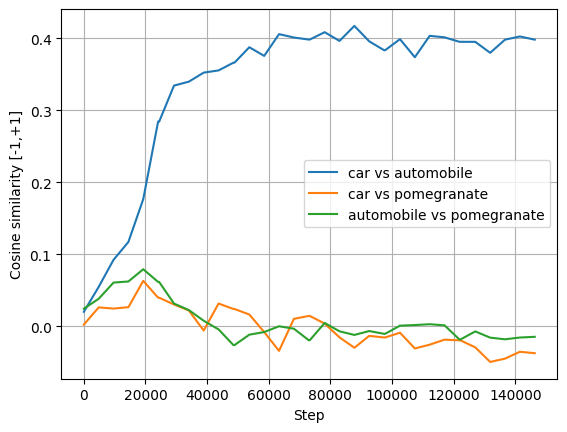
\includegraphics[width=0.6\textwidth]{img/pomegranate-test.png}
    \caption{Pomegranate test during the base model training}
    \label{fig:pomegranate-test}
\end{figure}


\subsection{Closest Neighbors Test}
Another quick test we conduct at the end of the training is checking the closest neighbors for 5 selected words, using the final model. This is an evaluation technique implemented with the inspiration from the article \cite{levy-dependency}, where the authors refer to this technique as "\textit{Qualitative Evaluation}" and use it to show how different models reflect different aspects of words. They limit their observations to 5 neighbors, but we extend it to 10 neighbors. For each word, the closest neighbor appears to be the word itself, we exclude them from the results. These closest neighbors are selected according to the cosine similarity of their target representations to the test word target representation. These five words are \textit{car}, \textit{money}, \textit{flower}, \textit{japan}, and \textit{suspicious}. The results obtained from our base model are given in Table \ref{tab:neighbors_test}.

\begin{table}[ht]
\centering
\begin{tabular}{|c|c|c|c|c|}
\hline
\rowcolor[HTML]{330001} 
{\color[HTML]{FFFFFF} car} & {\color[HTML]{FFFFFF} money} & {\color[HTML]{FFFFFF} flower} & {\color[HTML]{FFFFFF} japan} & {\color[HTML]{FFFFFF} suspicious} \\ \hline
\rowcolor[HTML]{E2EFDA} 
chevrolet                  & demand                       & perennials                    & daigo                        & parchamis                         \\ \hline
cars                       & pricing                      & cultivation                   & taiwan                       & plebs                             \\ \hline
\rowcolor[HTML]{E2EFDA} 
motor                      & dividends                    & sunflower                     & niigata                      & pdpa                              \\ \hline
bmw                        & loans                        & hibiscus                      & korea                        & parcham                           \\ \hline
\rowcolor[HTML]{E2EFDA} 
driver                     & profits                      & petals                        & meiji                        & negotiating                       \\ \hline
nhra                       & tax                          & sepals                        & prefecture                   & confidence                        \\ \hline
\rowcolor[HTML]{E2EFDA} 
motors                     & repay                        & edible                        & japanese                     & khalq                             \\ \hline
automobile                 & bonuses                      & flowers                       & takano                       & blamed                            \\ \hline
\rowcolor[HTML]{E2EFDA} 
chassis                    & cheques                      & shrubs                        & kitakyushu                   & advisers                          \\ \hline
\end{tabular}
\caption{Closest neighbors test on the base model}
\label{tab:neighbors_test}
\end{table}

Note that these neighbors are not listed in a particular order or ranking.
    %!TEX root = ../main.tex

\chapter{Experiments and Evaluations}
\label{chp:experiments}

What we have explained up to this chapter, model design and training, covers a relatively small part of the timeline of this study. We spent most of our time trying to understand the behavior of the produced models, collecting data about these behaviors, visualizing them, and comparing them with each other. 

The design and the implementation we have described up to this point refer to our base model, which is the model we used as the starting point and the reference for the other variants we produced with little adjustments and extra features. In this chapter, we will describe the other models we have developed. Next, we will select 4 top performers among them, and provide a more in-depth analysis regarding their behaviors and performances. Finally, we will talk about other experiments we conducted to explore our third-order model further.

\section{Data}
\label{sec:train_data}

Firstly, we will describe the data we use to train our model. We use a dataset called \verb|text8|, which was created by Matt Mahoney \cite{text8}. It is the first 100,000,000 bytes of plain text data obtained by truncating another file (\verb|fil9|, 715 MB) containing data from English Wikipedia \footnote{For details: \url{https://mattmahoney.net/dc/textdata.html}}. For ease of use, it is cleaned, meaning all the tables, links, citations, footnotes, and markups have been removed and hypertext links, numbers, and image captions are converted to ordinary text. The author describes the purpose of this dataset as a way to allow quicker testing, but we concluded this size of a corpus is sufficient and ideal considering the scope of our work and resources.

This dataset contains 17,005,207 tokens with 253,854 types. After the preprocessing (described in \ref{sec:preprocessing}), we are left with 8,448,361 tokens and 63,459 types. Then after the subsampling (described in \ref{sec:subsampling}), we have 3,428,264 tokens and 253,854 types. Finally, after the training/validation split (described in Section \ref{sec:val_split}), we have 3,085,438 tokens for the training, and 340,822 tokens for validating, using the same number of types.

\section{Model variants}
\label{sec:variants}
In addition to our base model, we have trained numerous other versions. We have kept the ones that yielded acceptable results for further analysis. By this, we are left with 26 versions of our model. In this section, we will briefly describe what is different in each version. Before we start, we should note that all of these models employ the same text preprocessing (See Section \ref{sec:preprocessing}), but they differ in what other processes they apply to the training data, training hyperparameters we choose for them, and the tricks they employ in their training loop.

For reference, here are some of the hyperparameters and tricks used in our base model:
\begin{itemize}
    \item Subsampling is enabled with a subsampling threshold of $1e-5$.
    \item Low context removal is disabled.
    \item Embedding vectors are in $300$ dimensions.
    \item Dynamic context windows with $L=4$.
    \item Negative training samples per each positive sample, i.e. parameter $k$, is set to $5$.
    \item The validation set is $10\%$ of the corpus.
    \item Each batch consists of $128$ target words. (\verb|batch_size| = $128$)
    \item We run the training for $6$ epochs.
    \item Our learning rate is $0.003$.
    \item We use \verb|Adam| optimizer with no learning rate scheduling.
    \item The weights of $\myscore{+}{w, u_1, u_2}$ and $\myscore{-}{w, u_1, u_3}$ are the same in the calculation of the overall loss.
    \item The loss function is constructed exactly like how it is described in Section \ref{sec:loss}.
\end{itemize}

Now when we describe other variants, we will only mention what is different, without going into any further detail. In the following numbered list, each item index corresponds to a version number.

\begin{enumerate}
    \item Corresponds to the base model.
    \item Learning rate is increased to $0.004$, with a decay coefficient of $0.85$.
    \item Context window size $L$ is adjusted to the number of occurrences of the word in the corpus, to assign every word in the training set a somewhat similar number of context words.
    \item Low context removal enabled with low context threshold of $100$.
    \item Subsampling threshold is increased to $1e-4$.
    \item In the loss function, instead of softplus, we use shifted \ac{ReLU} (Similar to SReLU in \cite{srelu}) with a shifting factor of $+1e-5$.
    \item Trying for a lucky initialization. Before we kick off the training loop, we try out $500$ random initializations and select the one with minimal loss for the training.
    \item Can a smaller batch size add to the ability of generalization? Batch size is lowered down to $64$.
    \item If we use a larger batch size to utilize our GPU resources better, how will it affect our model performance? To investigate this, the batch size is increased to $256$.
    \item Negative correction to the $\myscore{+}{w, u_1, u_2}$, for making sure if our implementation is correct.
    \item Replacing the softplus function in our loss with the Gaussian function\footnote{For details, see \url{https://en.wikipedia.org/wiki/Gaussian_function}}, followed by clamping the minimum to $1e-40$.
    \item Do the negative samples overpower the positive ones? Using a coefficient of $0.5$ for the $\myscore{-}{w, u_1, u_3}$ in the loss calculation.
    \item Using a coefficient of $0.2$ for the $\myscore{-}{w, u_1, u_3}$ in the loss calculation.
    \item Will regularization help us? Adding a dropout layer to the target and context embeddings. In other words, calculating loss using the embedding vectors with randomly disabled weights. The dropout rate is set to $0.4$ for both matrices.
    \item Applying dropout only to the target embeddings, again with the dropout rate of $0.4$.
    \item Using only $\myscore{+}{w, u_1, u_2}$.
    \item Deriving the calculation of $\myscore{-}{w, u_1, u_3}$ from the calculation of $\myscore{+}{w, u_1, u_2}$.
    \item Simplifying the loss function: Eliminating softplus from $\myscore{-}{w, u_1, u_3}$ and apply sigmoid directly to $D = P_\mathit{context} - P_\mathit{noise}$.
    \item Again eliminating softplus from $\myscore{-}{w, u_1, u_3}$, and replacing softplus with \ac{ReLU} in $\myscore{+}{w, u_1, u_2}$.
    \item Again eliminating softplus from $\myscore{-}{w, u_1, u_3}$, and replacing softplus with absolute function in $\myscore{+}{w, u_1, u_2}$.
    \item Rethinking our 3rd order loss: Conversion to the 2nd order with converging context projections to a $\delta$ value, and pushing the noise projections to the left. ($\delta = 5$)
    \item Same as the previous version, but this time $\delta$ is a random integer sampled from $[2,10]$ for each batch.
    \item Shifting weights for $\myscore{+}{w, u_1, u_2}$ and $\myscore{-}{w, u_1, u_3}$ in loss calculation. $w_p$ is the weight of $\myscore{+}{w, u_1, u_2}$, and $w_n$ is for $\myscore{-}{w, u_1, u_3}$. Training starts with the values $w_p = 0.92$, $w_n = 0.08$. It slowly shifts values until at the end of the training we reach $w_p = 0.5$, $w_n = 0.5$.
    \item Same as the previous one, but this time the values of $w_n$ and $w_p$ are switched.
    \item We again use weights for $\myscore{+}{w, u_1, u_2}$ and $\myscore{-}{w, u_1, u_3}$. But this time, we start by $w_p = 0.0$ and $w_n = 1.0$. Until the end of the training, these weights flip at every epoch.
    \item Eliminating $\myscore{+}{w, u_1, u_2}$ and only using the simplified version (only sigmoid, no softplus) of $\myscore{-}{w, u_1, u_3}$.
\end{enumerate}

We kept these models and eliminated some other versions because these were the ones that showed an acceptable performance and a reasonable learning curve in the training loop. Most of these models show similar performances, while the rest are slightly less impressive. It will be a waste of space and not be so useful to describe how every model performs and what their learning curves look like. Therefore we decided to pick the base model and a few other top performers and move on with this chapter using only them.


\section{Analysis of top four performers}

Now that we have shared the ideas we have experienced with, we can outline the behaviors and capabilities of these models. For this section, we decided to move with four models, namely, the \textbf{base model}, \textbf{version 15}, \textbf{version 18}, and \textbf{version 26}. We based our decision on the selection of these models to our immediate evaluations (see Section \ref{sec:immediate}), learning curves, and their scores on the word similarity task using the \verb|WordSim353| dataset. More about this dataset will be provided later in this section. As we mentioned earlier, a lot of our versions yield very similar performances. In those cases, we favored the models that were produced with more distinct ideas.

\subsection{Learning curves and immediate evaluations}
Before further analysis, we will first share how these models learned and how they performed in our immediate evaluations.

Table \ref{tab:loss_curves} shows the loss curves for all 4 models, throughout the 6 epochs.

\begin{table}[ht]
  \centering
  \begin{tabular}{cc}
    \begin{subfigure}{0.45\textwidth}
      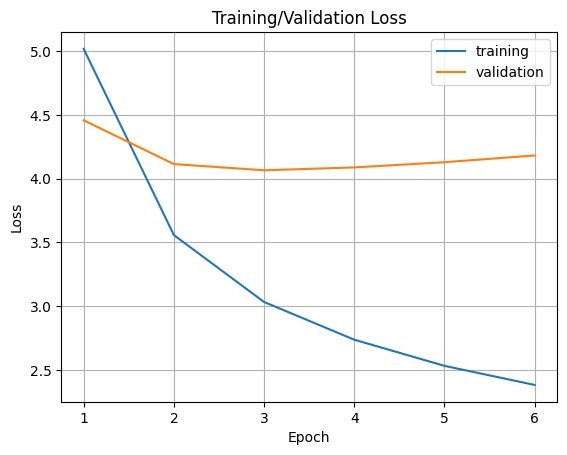
\includegraphics[width=\linewidth]{img/curve_base.png}
      \caption{Base Model}
    \end{subfigure} & 
    \begin{subfigure}{0.45\textwidth}
      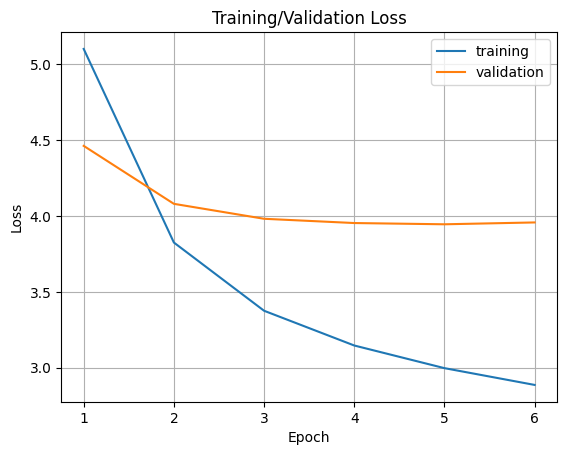
\includegraphics[width=\linewidth]{img/curve_15.png}
      \caption{Version 15}
    \end{subfigure} \\
    \begin{subfigure}{0.45\textwidth}
      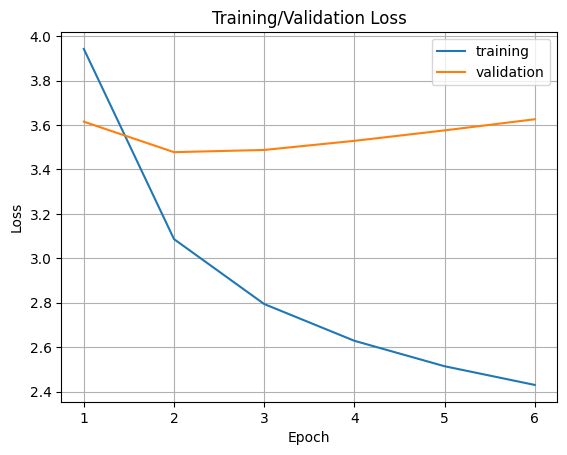
\includegraphics[width=\linewidth]{img/curve_18.png}
      \caption{Version 18}
    \end{subfigure} & 
    \begin{subfigure}{0.45\textwidth}
      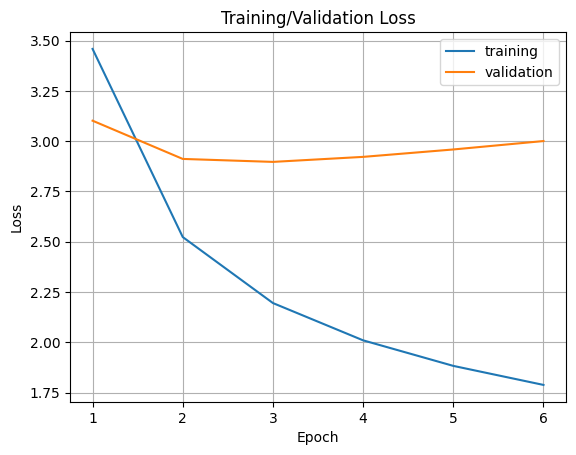
\includegraphics[width=\linewidth]{img/curve_26.png}
      \caption{Version 26}
    \end{subfigure}
  \end{tabular}
  \caption{Training and validation loss curves for each model}
  \label{tab:loss_curves}
\end{table}

We see that for all models, the loss of the training data keeps going down until the end. However, this is not the case for the validation loss. Except for version 15, we see no improvement, in contrast, we see a slight deterioration in the validation loss. This tells us that our model fits too well to the occurrences in the training partition in just a few epochs so that it fails to recognize how these words could have been positioned in any other piece of text outside of this data. This is a clear indication of overfitting. %However, we are hesitant to conclude the models are in a better state at the end of the third epoch, than how they are at the end of the training loop.

For the case of version 15, we see that regularization with the dropout layer adds up to the model's generalization abilities. We cannot complain about what the validation loss curve looks like by the end of 6 epochs.

As the differences between these models are mainly about the way they calculate their losses, the numerical values of losses are not directly comparable. The only meaningful comparison could be between the base model and the model version 15, which we see even though the base model has a better training loss, version 15 performs better on the validation data.

Now we show the performances of these models on our immediate evaluations (see Section \ref{sec:immediate}).

\begin{table}[ht]
  \centering
  \begin{tabular}{cc}
    \begin{subfigure}{0.45\textwidth}
      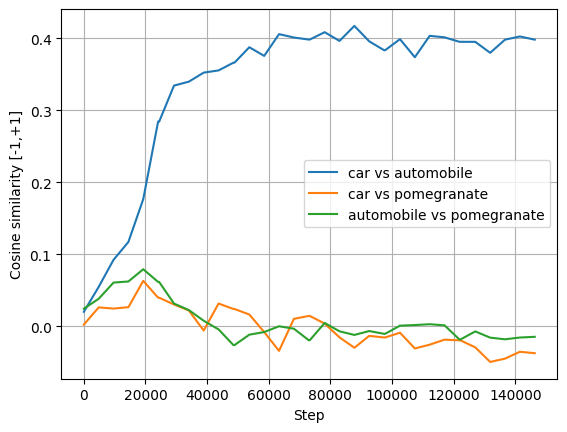
\includegraphics[width=\linewidth]{img/pom_base.png}
      \caption{Base Model}
    \end{subfigure} &
    \begin{subfigure}{0.45\textwidth}
      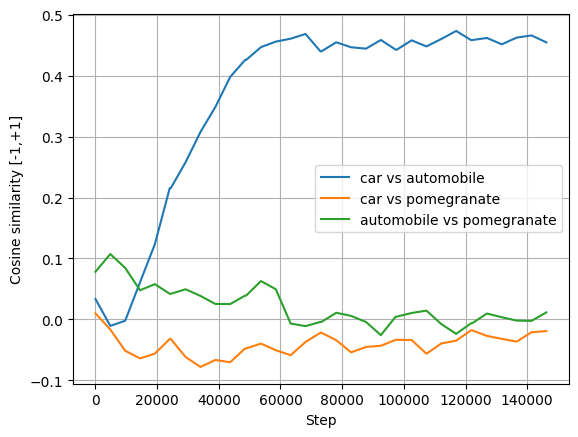
\includegraphics[width=\linewidth]{img/pom_v15.png}
      \caption{Version 15}
    \end{subfigure} \\
    \begin{subfigure}{0.45\textwidth}
      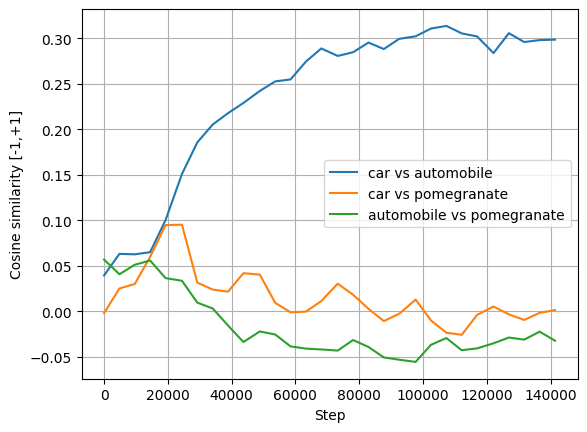
\includegraphics[width=\linewidth]{img/pom_v18.png}
      \caption{Version 18}
    \end{subfigure} &
    \begin{subfigure}{0.45\textwidth}
      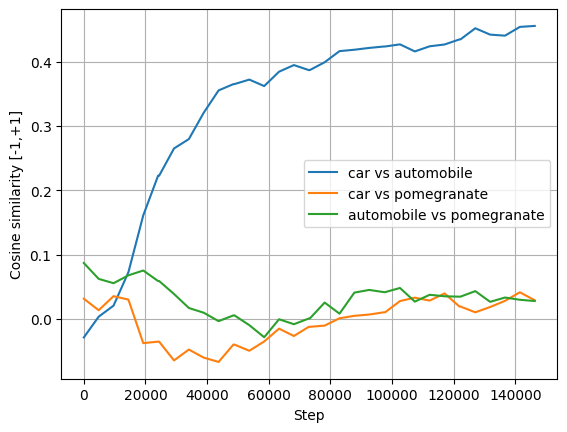
\includegraphics[width=\linewidth]{img/pom_v26.png}
      \caption{Version 26}
    \end{subfigure}
  \end{tabular}
  \caption{Cosine similarity-based immediate evaluations of models}
  \label{tab:pom_plots}
\end{table}

In Table \ref{tab:pom_plots}, we show how our models improve as they learn according to our cosine similarity-based evaluation. We see that each of these models can easily distinguish what should be similar and what should not from very early on, leaving a good impression before we move to large-scale similarity-based evaluations. Next, we share the closest neighbors to our test words, according to our selected models.

% BASE
\begin{table}[!ht]
\centering
\begin{tabular}{|c|c|c|c|c|}
\hline
\rowcolor[HTML]{330001} 
{\color[HTML]{FFFFFF} car} & {\color[HTML]{FFFFFF} money} & {\color[HTML]{FFFFFF} flower} & {\color[HTML]{FFFFFF} japan} & {\color[HTML]{FFFFFF} suspicious} \\ \hline \rowcolor[HTML]{E2EFDA} 
chevrolet & demand & perennials  & daigo & parchamis \\ \hline
cars & pricing & cultivation & taiwan & plebs  \\ \hline \rowcolor[HTML]{E2EFDA} 
motor & dividends  & sunflower & niigata & pdpa   \\ \hline
bmw & loans & hibiscus & korea & parcham \\ \hline \rowcolor[HTML]{E2EFDA} 
driver & profits & petals & meiji & negotiating \\ \hline
nhra & tax & sepals & prefecture & confidence \\ \hline \rowcolor[HTML]{E2EFDA} 
motors & repay & edible & japanese & khalq  \\ \hline
automobile & bonuses & flowers & takano & blamed \\ \hline \rowcolor[HTML]{E2EFDA} 
chassis  & cheques & shrubs & kitakyushu & advisers \\ \hline
\end{tabular}
\caption{Closest neighbors evaluation for the base model}
\label{tab:base-neighbors}
\end{table}

% V15
\begin{table}[!ht]
\centering
\begin{tabular}{|c|c|c|c|c|}
\hline
\rowcolor[HTML]{330001} 
{\color[HTML]{FFFFFF} car} & {\color[HTML]{FFFFFF} money} & {\color[HTML]{FFFFFF} flower} & {\color[HTML]{FFFFFF} japan} & {\color[HTML]{FFFFFF} suspicious} \\ \hline \rowcolor[HTML]{E2EFDA} 
mercedes & securities & pear & tokyo & qaida  \\ \hline
truck & profits & petals & honshu & told   \\ \hline \rowcolor[HTML]{E2EFDA} 
mans & gambling & foliage & japanese & campaign \\ \hline
coupe & wages & stalks & korea & corrupt \\ \hline \rowcolor[HTML]{E2EFDA} 
automobile & dollars & fruit & manchuria  & harshly \\ \hline 
cars & depositors & bees & china & resignations \\ \hline \rowcolor[HTML]{E2EFDA} 
chevrolet & exploitative & flowers & meiji & dissenters \\ \hline
daytona  & price & larvae & indonesia  & scorched \\ \hline \rowcolor[HTML]{E2EFDA} 
driver & repay & buckwheat & tokugawa & nationalists \\ \hline 
\end{tabular}
\caption{Closest neighbors evaluation for version 15}
\label{tab:v15-neighbors}
\end{table}

% V18
\begin{table}[!ht]
\centering
\begin{tabular}{|c|c|c|c|c|}
\hline
\rowcolor[HTML]{330001} 
\multicolumn{1}{|c|}{\cellcolor[HTML]{330001}{\color[HTML]{FFFFFF} car}} & \multicolumn{1}{c|}{\cellcolor[HTML]{330001}{\color[HTML]{FFFFFF} money}} & \multicolumn{1}{c|}{\cellcolor[HTML]{330001}{\color[HTML]{FFFFFF} flower}} & \multicolumn{1}{c|}{\cellcolor[HTML]{330001}{\color[HTML]{FFFFFF} japan}} & \multicolumn{1}{c|}{\cellcolor[HTML]{330001}{\color[HTML]{FFFFFF} suspicious}} \\ \hline
\rowcolor[HTML]{E2EFDA} 
mans & price & mentha & hirohito  & ilyas \\ \hline
driver & sell & corolla & kansai & detractors \\ \hline
\rowcolor[HTML]{E2EFDA} 
chassis  & prices & hibiscus & maldives & inappropriately \\ \hline 
engined  & spending  & shrubs & taiwan & justified \\ \hline
\rowcolor[HTML]{E2EFDA} 
cars & liquidity & kiwifruit & svalbard & tensions \\ \hline
miata & earnings  & snowmen & toshiki & alarmed \\ \hline
\rowcolor[HTML]{E2EFDA} 
benz & profit & laurel & dynasties & pledges  \\ \hline
mercedes & issuer  & leaf & nmt & assurances \\ \hline
\rowcolor[HTML]{E2EFDA} 
bmw & monetary & vines & korea  & accept \\ \hline
\end{tabular}
\caption{Closest neighbors evaluation for the version 18}
\label{tab:v18-neighbors}
\end{table}

%V26
\begin{table}[!ht]
\centering
\begin{tabular}{|c|c|c|c|c|}

\hline \rowcolor[HTML]{330001} 
\textcolor[HTML]{FFFFFF}{car} & \textcolor[HTML]{FFFFFF}{money} & \textcolor[HTML]{FFFFFF}{flower} & \textcolor[HTML]{FFFFFF}{japan} & \textcolor[HTML]{FFFFFF}{suspicious} \\ \hline \rowcolor[HTML]{E2EFDA} 

miata & loans & cucumber & nagano & shia \\ \hline
driver & taxes & stamens & hong & evocation \\ \hline \rowcolor[HTML]{E2EFDA} 
automobile & monetary & floral & singapore & azzam \\ \hline 
truck & borrow & foliage & china & leftist \\ \hline \rowcolor[HTML]{E2EFDA} 
crash & wages & petals & kyushu & denied \\ \hline
engined & fund & inflorescence & osaka & walid \\ \hline \rowcolor[HTML]{E2EFDA} 
cars & funds & sepals & japanese & refusing \\ \hline
chassis & earnings & hibiscus & meiji & entrenched \\ \hline \rowcolor[HTML]{E2EFDA} 
chevrolet & payments & strawberry & tokyo & shehri \\ \hline

\end{tabular}
\caption{Closest neighbors evaluation for the version 26}
\label{tab:v26-neighbors}
\end{table}


\subsection{Statistics: Performance and characteristics}
\label{sec:stats}

We believe that the best way to understand the behavior of our models is to observe how they organize the vectors in the vector space, and how these behaviors change as they learn. For this purpose, we gathered the models we saved at the end of each epoch, computed some statistics, and tried to see if we could find any useful trend embedded in these numbers.

To keep a balance between computational efficiency and the fair representation of the vector space, we sampled a subset of words from our vocabulary to conduct our computations.

\begin{figure}[ht]
    \centering
    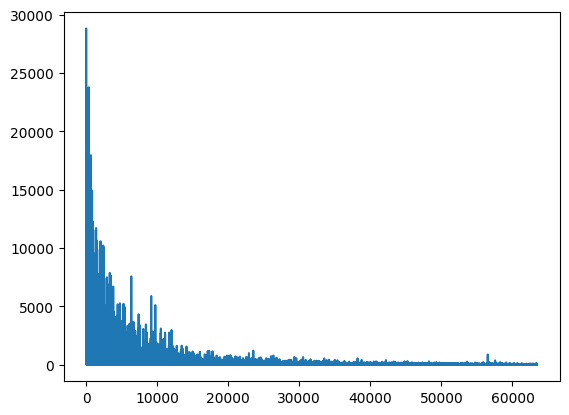
\includegraphics[width=0.7\textwidth]{img/word_counts.png}
    \caption{Word frequencies in our training corpus.}
    \label{fig:word_counts}
\end{figure}

Figure \ref{fig:word_counts} shows the frequencies of the types in our vocabulary in the corpus, partially sorted from the most frequent to the least. We decided that instead of sampling $n$ words from anywhere in the corpus, it would be more logical to select a frequency range that represents the average case and sample our test words from there. Following this, we sampled $50$ words from the set of words that appear in our corpus $f$ times, where $f \in [100, 20000]$. 5 of these test words are:

\begin{displayquote}
\centering
'televised', 'uruguayan', 'credits', 'geologist', 'commerce'
\end{displayquote}

Next, for all of our test words, we collected all the words that appear in their context windows and also sampled some noise words. Then for each test word, we picked the 100 most frequent context words and the 100 most frequent noise words and eliminated the rest. Now that we have our target words, combined with their context and noise samples, we are ready to proceed to our computations.

We have selected 6 statistics that we believe can give us useful insights and expose some interesting patterns. These 6 statistics are:

\begin{enumerate}
    \item Average context word (context representation) projections onto the target word (target representation).
    \item Average noise word (context representation) projections onto the target word (target representation).
    \item Average \textbf{variance} of the context words (context representation) projections onto the target word (target representation).
    \item Average projection \textbf{difference} of the context words (context representation) and the noise words (context representation) onto the target word (target representation).
    \item Average \textbf{cosine similarity} of a context word (target representation) and the target word (target representation).
    \item Average target word (target representation) magnitude.
\end{enumerate}

For each model, we calculated these statistics, for all of its models produced at the end of each 6 epochs. Also to give a better view, we conducted the same calculations for a random model, you will see it as "Epoch 0" in the plots. All the statistics listed above are visualized for our selected four models in Figure \ref{fig:stats_base}, Figure \ref{fig:stats_v15}, Figure \ref{fig:stats_v18}, and Figure \ref{fig:stats_v26}, for the base model, version 15, version 18, and version 26, respectively. You will notice that the plots are designed to show how these metrics change starting from the random initialization to the final epoch. The numbers used in the labels correspond to the indexes used in the above list. 

\begin{figure}[!ht]
    \centering
    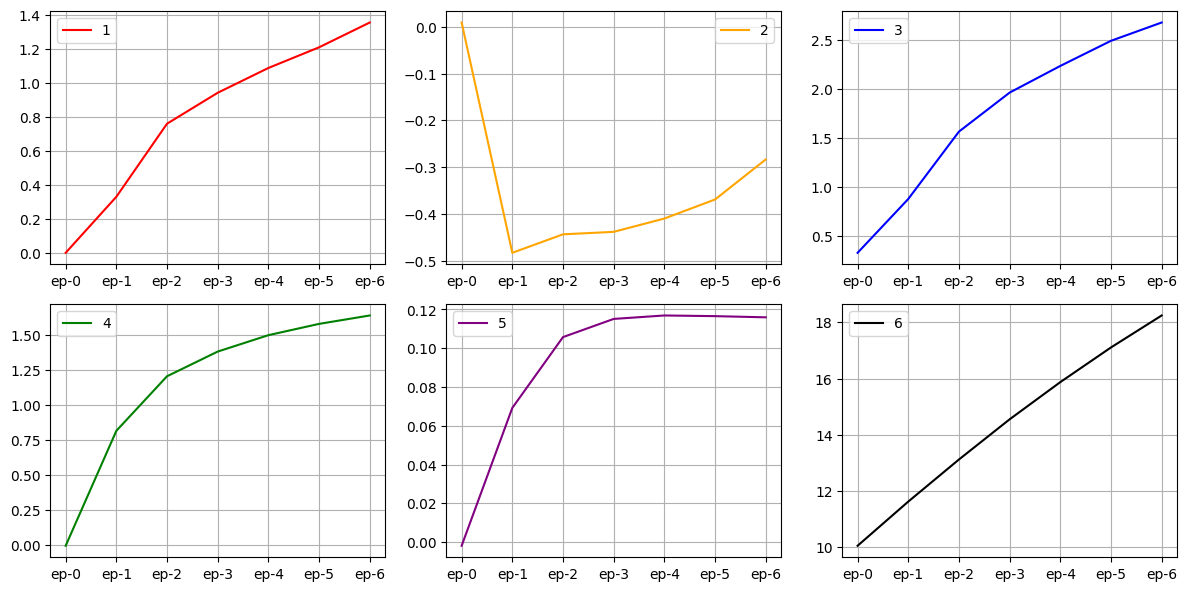
\includegraphics[width=1.0\textwidth]{img/stats_base.png}
    \caption{Statistics for the base model}
    \label{fig:stats_base}
\end{figure}

\begin{figure}[!ht]
    \centering
    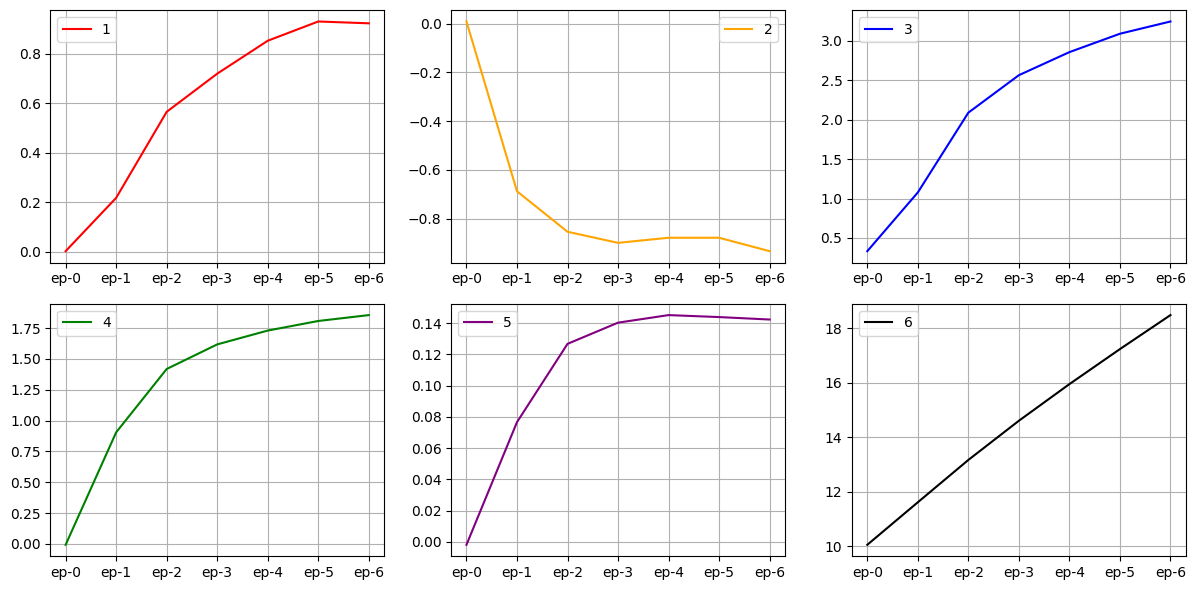
\includegraphics[width=1.0\textwidth]{img/stats_v15.png}
    \caption{Statistics for version 15}
    \label{fig:stats_v15}
\end{figure}

\begin{figure}[!ht]
    \centering
    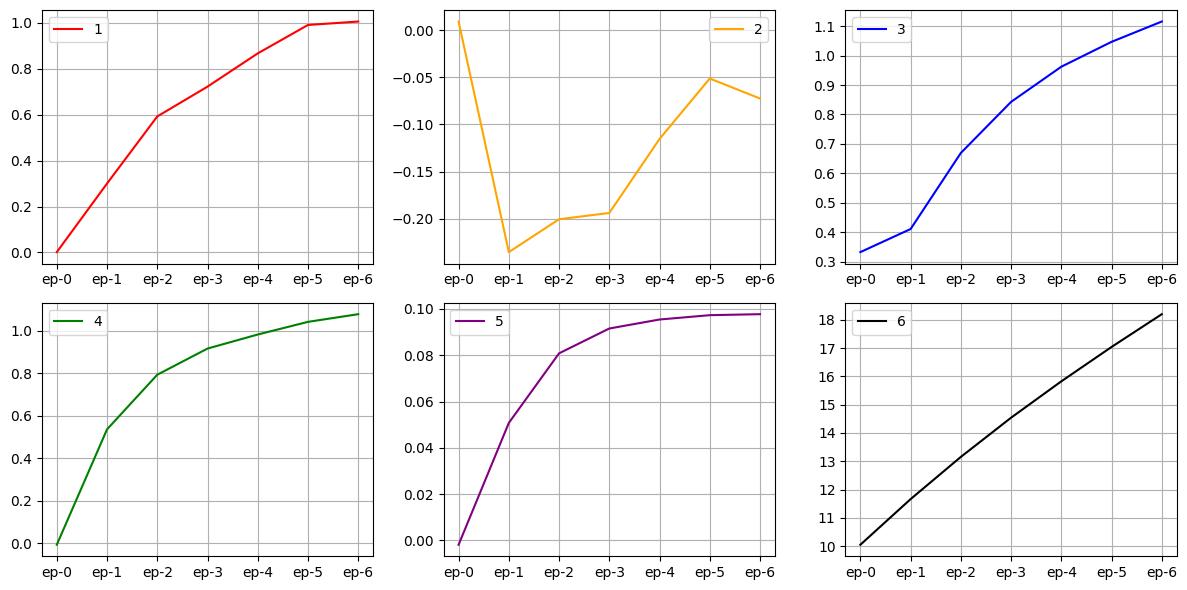
\includegraphics[width=1.0\textwidth]{img/stats_v18.png}
    \caption{Statistics for version 18}
    \label{fig:stats_v18}
\end{figure}

\begin{figure}[!ht]
    \centering
    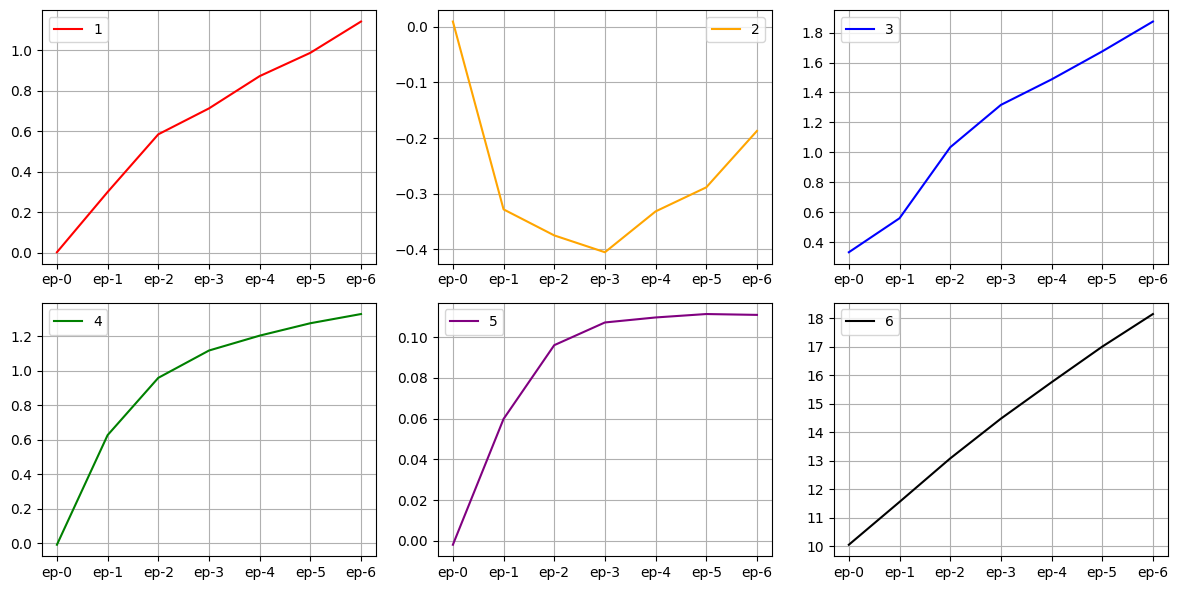
\includegraphics[width=1.0\textwidth]{img/stats_v26.png}
    \caption{Statistics for version 26}
    \label{fig:stats_v26}
\end{figure}


To commentate on what we see in these figures, the first thing we notice is that the trends followed by each model for every metric are somewhat similar to each other. For instance, we see that the statistic \#1 for each model goes up as the learning progresses. On the other hand, we see that statistic \#2 tends to go down with the learning, but for some models, it starts to go up after some point. We observe this increasing trend for all the models except for version 15. Oddly enough, version 15 is the only model in which we did not observe an increasing trend in its validation loss curve, which makes us think that these two observations are correlated.

Another thing we notice is that for all models, the variances of the context projections go up as the learning progresses. We are not able to interpret this with full confidence, because this might indicate several things. For one, which is the favored case, this might mean that we are creating context hyperplanes, and these groups of projections are becoming more and more distanced from each other. Another possibility is that our context projections are getting spread over the target vector, following no particular rule or trend.

We also see that our loss function, regardless of the version, makes our target vectors longer and longer, with a stable pace. 

Finally, the thing that we are glad to see the most is statistic \#4, which tells us that our loss function successfully pushes the noise projections to the left side of the context projections. Plus, this increase in projection difference keeps going up even when statistic \#2 starts following an increasing trend. 


\subsection{Visualizing vector projections}
\label{sec:vis_proj}

We now visualize the vector projections of the context and the noise words onto the target vectors of our test words. We randomly chose 20 target words from our test words for this task and calculated the orthogonal projections of the context vectors of the context and the noise words for each epoch. This will enable us to demonstrate how the vector space is organized as the model learns better about the training data.

For the sake of simplicity of our demonstration, we will share the projections of 3 target words instead of 20. In the following plots, you will find a bunch of green and red dots stacked together on different rows. Green dots represent the context projections, and the red dots represent the noise projections. Each dot from both colors represents an orthogonal projection of a context vector (context word or a noise word) onto the target vector. Context vector projections are stacked in a way so that the bottom row corresponds to the initialization and the topmost row corresponds to the last epoch. For the noise projections, it is the opposite, with the topmost row corresponding to the initialization and downward proceeding with the next epoch until the bottom-most. 

The blue lines in the middle of the figures represent the target vector. We can see which target are we looking at from the label placed on the top right corner of each figure. The numbers on the left side of the figures have no meaning. In addition, the black dots placed towards the middle of the group in each row show where the average of that row falls. For lines showing the same epochs, lines were drawn to describe the relative positions of the averages between the corresponding context and noise lines. 

\begin{table}[p]
  \centering
  \begin{tabular}{cc}
    \begin{subfigure}{0.95\textwidth}
      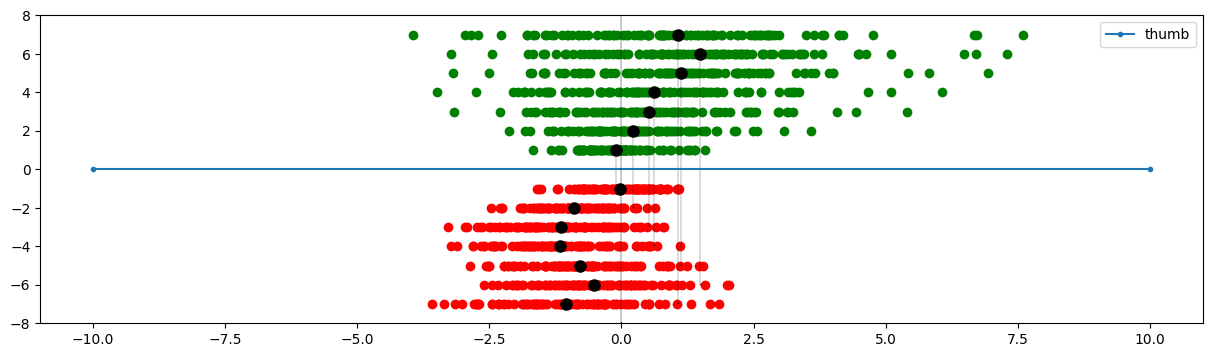
\includegraphics[width=\linewidth]{img/thumb_base.png}
      \caption{Target word: Thumb}
    \end{subfigure} \\
    \begin{subfigure}{0.95\textwidth}
      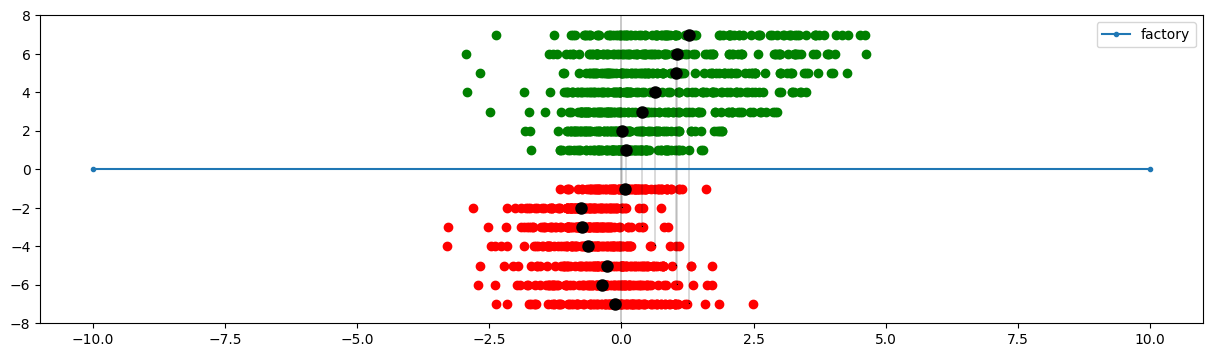
\includegraphics[width=\linewidth]{img/factory_base.png}
      \caption{Target word: Factory}
    \end{subfigure} \\
    \begin{subfigure}{0.95\textwidth}
      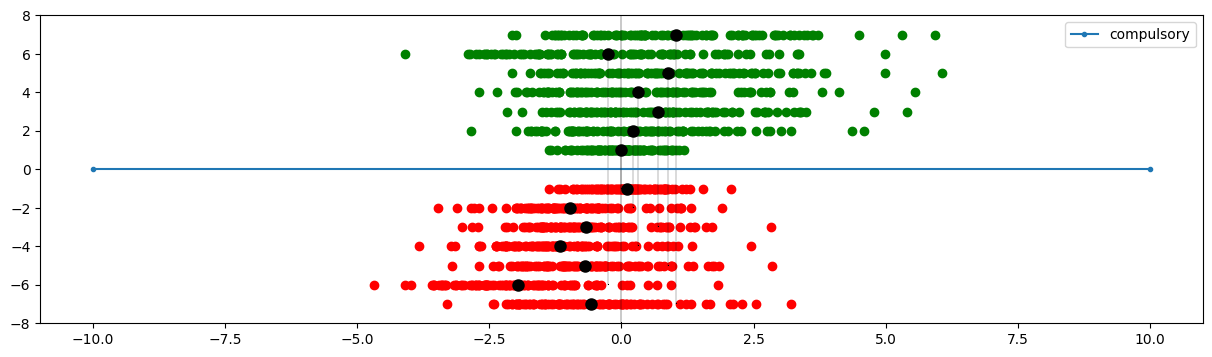
\includegraphics[width=\linewidth]{img/compulsory_base.png}
      \caption{Target word: Compulsory}
    \end{subfigure} 
  \end{tabular}
  \caption{Context and noise projections onto the target vector - Base Model}
  \label{tab:base_projections}
\end{table}


\begin{table}[p]
  \centering
  \begin{tabular}{cc}
    \begin{subfigure}{0.95\textwidth}
      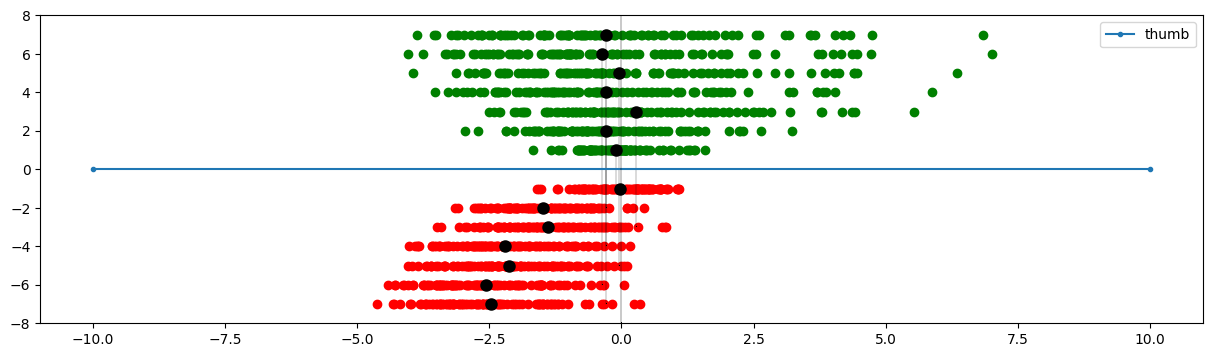
\includegraphics[width=\linewidth]{img/thumb_v15.png}
      \caption{Target word: Thumb}
    \end{subfigure} \\
    \begin{subfigure}{0.95\textwidth}
      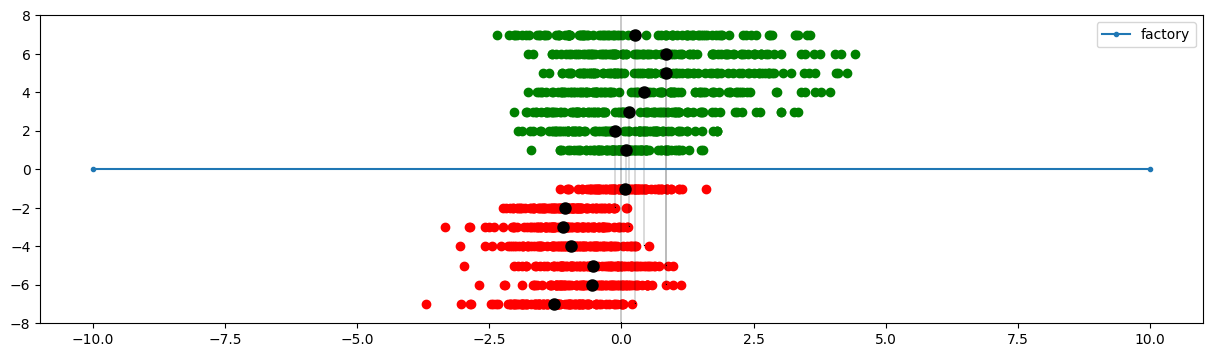
\includegraphics[width=\linewidth]{img/factory_v15.png}
      \caption{Target word: Factory}
    \end{subfigure} \\
    \begin{subfigure}{0.95\textwidth}
      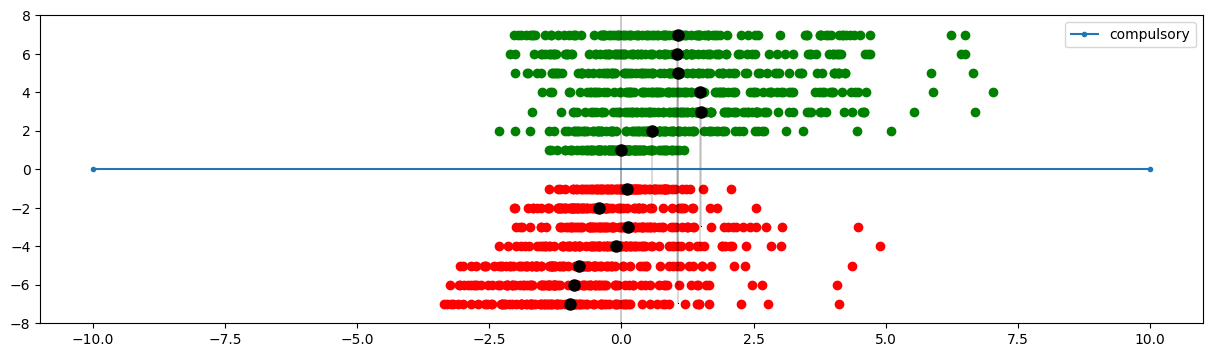
\includegraphics[width=\linewidth]{img/compulsory_v15.png}
      \caption{Target word: Compulsory}
    \end{subfigure} 
  \end{tabular}
  \caption{Context and noise projections onto the target vector - Version 15}
  \label{tab:v15_projections}
\end{table}


\begin{table}[p]
  \centering
  \begin{tabular}{cc}
    \begin{subfigure}{0.95\textwidth}
      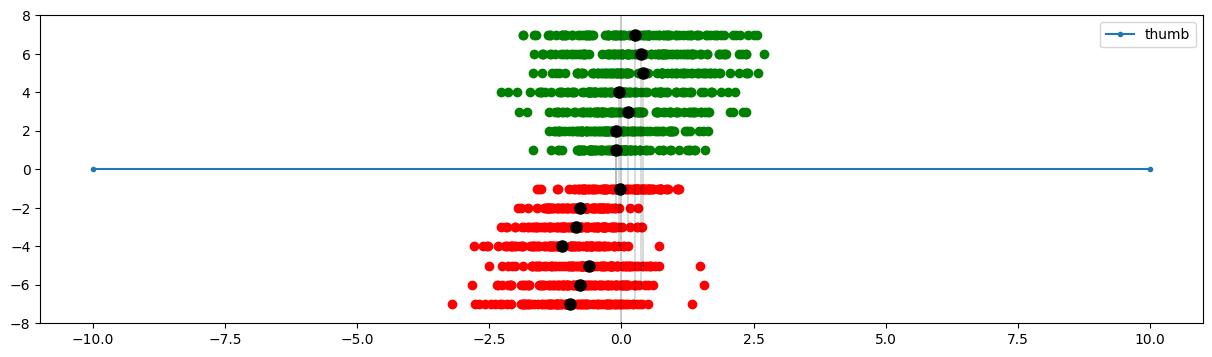
\includegraphics[width=\linewidth]{img/thumb_v18.png}
      \caption{Target word: Thumb}
    \end{subfigure} \\
    \begin{subfigure}{0.95\textwidth}
      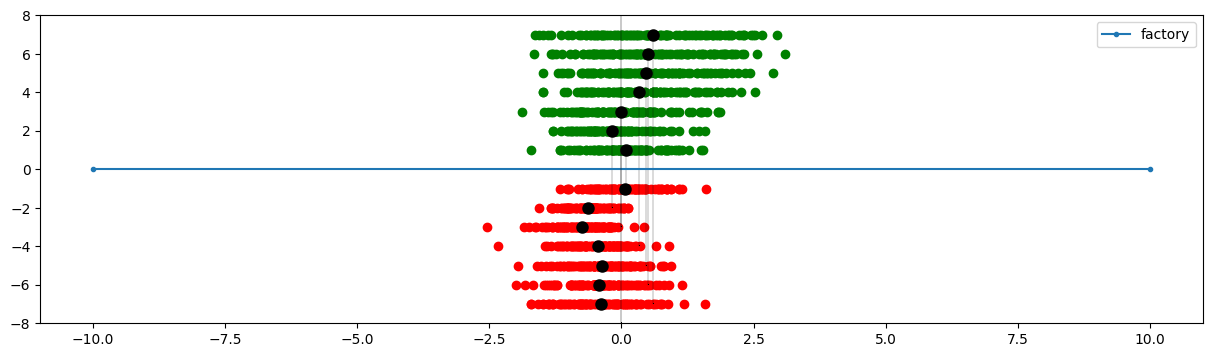
\includegraphics[width=\linewidth]{img/factory_v18.png}
      \caption{Target word: Factory}
    \end{subfigure} \\
    \begin{subfigure}{0.95\textwidth}
      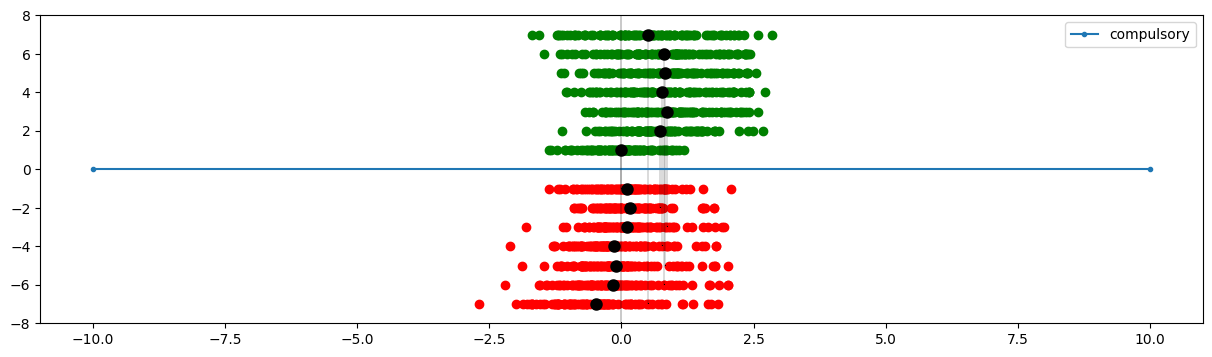
\includegraphics[width=\linewidth]{img/compulsory_v18.png}
      \caption{Target word: Compulsory}
    \end{subfigure} 
  \end{tabular}
  \caption{Context and noise projections onto the target vector - Version 18}
  \label{tab:v18_projections}
\end{table}


\begin{table}[p]
  \centering
  \begin{tabular}{cc}
    \begin{subfigure}{0.95\textwidth}
      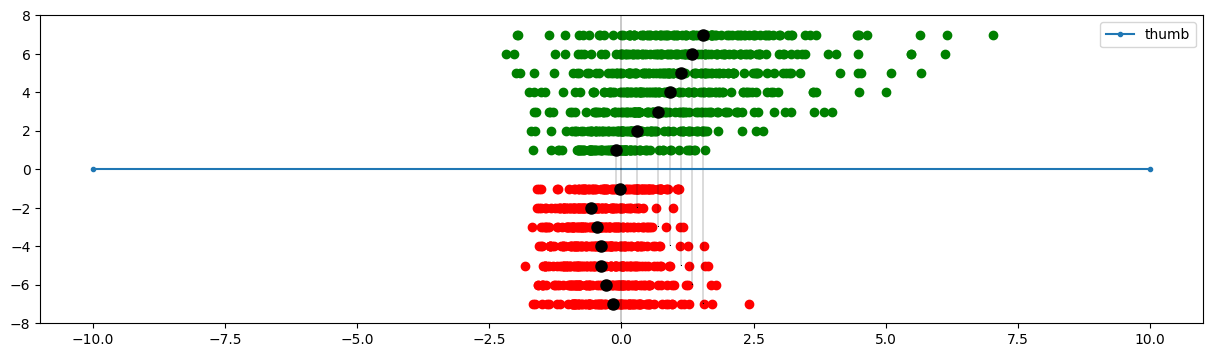
\includegraphics[width=\linewidth]{img/thumb_v26.png}
      \caption{Target word: Thumb}
    \end{subfigure} \\
    \begin{subfigure}{0.95\textwidth}
      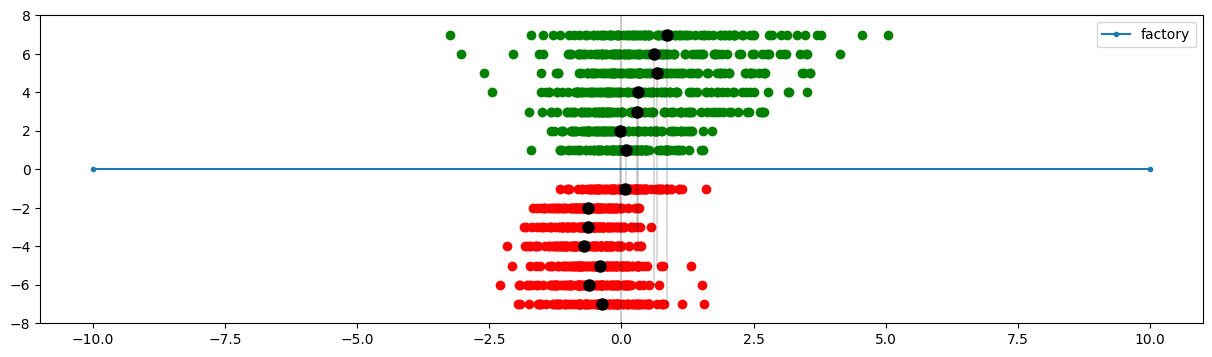
\includegraphics[width=\linewidth]{img/factory_v26.png}
      \caption{Target word: Factory}
    \end{subfigure} \\
    \begin{subfigure}{0.95\textwidth}
      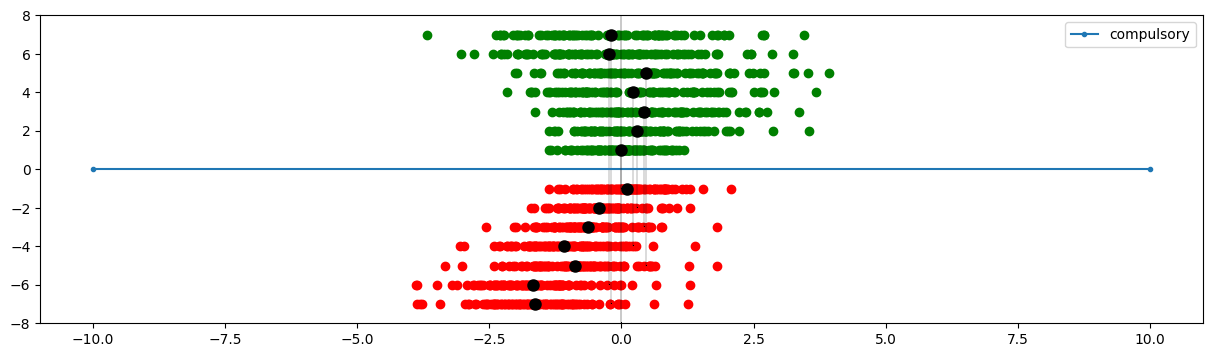
\includegraphics[width=\linewidth]{img/compulsory_v26.png}
      \caption{Target word: Compulsory}
    \end{subfigure} 
  \end{tabular}
  \caption{Context and noise projections onto the target vector - Version 26}
  \label{tab:v26_projections}
\end{table}

For three target words, "\textit{Thumb}", "\textit{Factory}" and "\textit{Compulsory}", we show the projections for each model in Table \ref{tab:base_projections}, Table \ref{tab:v15_projections}, Table \ref{tab:v18_projections}, and Table \ref{tab:v26_projections}.

Just like what we observed in the charts we presented earlier, we see that regardless of the shifting of the noise and context projections, the difference between them is always kept positive, and usually increases as epochs progress. It is interesting to see that sometimes we see noise word projections go right, or the context word projections go left, even though this is expected to diverge our loss. Nevertheless, even by doing this, seems like our models find the configuration that minimizes the loss better than the epoch before.

We see that the projections, especially the context word projections, get more and more spread with the learning. We fail to observe any obvious grouping of projections, which we believe would indicate the existence of context hyperplanes. 

We should note, however, that there is a possibility that a context word can be sampled also as a noise word in some of these plots. It is not very likely but we do not know for sure, and this can be the reason for outliers in some cases.

\subsection{Context word projections clustering}

% Maybe add a reference here
Aiming to find a hint of the existence of context hyperplanes, now we apply the k-means clustering algorithm to the context word projections. For all 50 test words and their context words we collected from our corpus, we calculate the context word projections onto the target embeddings of the test words. Then for each test word, we run the clustering algorithm on these projections. The k-means algorithm requires the number of clusters $k$ to be given beforehand. We run the clustering algorithm for different $k$ values, ranging between two and eight. This operation we described is conducted for all four models and each of their epochs.

We judge the quality of clusters given the values and $k$ using a metric called "\textit{Silhouette Score}". It is a metric that evaluates the compactness of the formed clusters, and the separation amongst them. From another perspective, it considers the similarity of an object to its cluster, compared to other clusters. This metric ranges between $[-1, 1]$, where $1$ is the most ideal clustering and $-1$ is the worst case.

For a single sample, let $a$ be the average intra-cluster distance and $b$ be the average nearest-cluster (except the cluster that the sample is assigned to) distance. The Silhouette Coefficient for a sample $s(i)$ is calculated as:

\[
s(i) = \frac{(b - a)}{\max(a, b)}
\]

The overall Silhouette Score $S$, which we use as the clustering score, is calculated as:

\[
S = \frac{\sum_{i \in P} s(i)}{|P|}
\]
\noindent
where $P$ is the full set of context projection values.

We calculated this score for each test word and for each epoch of each model. As the distribution of the projections is completely different for each word and in each model, it is not logical to calculate an average value among all test words. However, when we look at the clustering scores for each particular test word and model combination, we fail to see a clear clustering for any given $k$. Whatever is the $k$ value, we keep observing clustering scores ranging between 0.5 and 0.65, indicating that none of these $k$ values provide a clear grouping of these projection values. This means that we fail to prove the existence of context hyperplanes using a clustering approach.

We will omit the full list of results, but we share the scores for the test word "\textit{title}" for the final epochs of each model, in Table \ref{tab:title-clusters}. We observe similar results for every other case as well.

\begin{table}
\centering
\begin{tabular}{|c|c|c|c|c|}
\hline
\rowcolor[HTML]{330001} 
\cellcolor[HTML]{FFFFFF}{\color[HTML]{FFFFFF} }                 & {\color[HTML]{FFFFFF} base (Ep. 6)} & {\color[HTML]{FFFFFF} v15 (Ep. 6)} & {\color[HTML]{FFFFFF} v18 (Ep. 6)} & {\color[HTML]{FFFFFF} v26 (Ep. 6)} \\ \hline
\rowcolor[HTML]{FFFFFF} 
\cellcolor[HTML]{330001}{\color[HTML]{FFFFFF} Best k}           & 8                                     & 2                                    & 7                                    & 2                                    \\ \hline
\rowcolor[HTML]{FFFFFF} 
\cellcolor[HTML]{330001}{\color[HTML]{FFFFFF} Clustering Score} & 0.575                                 & 0.600                                & 0.597                                & 0.568                                \\ \hline
\end{tabular}
\caption{Clustering of context projections for the test word "title"}
\label{tab:title-clusters}
\end{table}


\subsection{Visualizing context projections}

Just to see what happens, now we employ a different approach and visualize the context projections, rather than the context word projections. The difference is that instead of visualizing the projections of each context word, we now calculate an average projection of each context of a test word and show that instead. A "context" of a word is the set of tokens that appear in the context window for one occurrence of that word. To be clearer, the projection of a context $c$ is:

\[
P(c) = \frac{\sum_{w \in c} p(w)}{|c|}
\]
\noindent
where $P(c)$ is the projection of the context $c$ and $p(w)$ is the projection of the context representation of the word $w$ onto the target representation of the target word.

\begin{table}[p]
  \centering
  \begin{tabular}{cc}
    \begin{subfigure}{0.95\textwidth}
      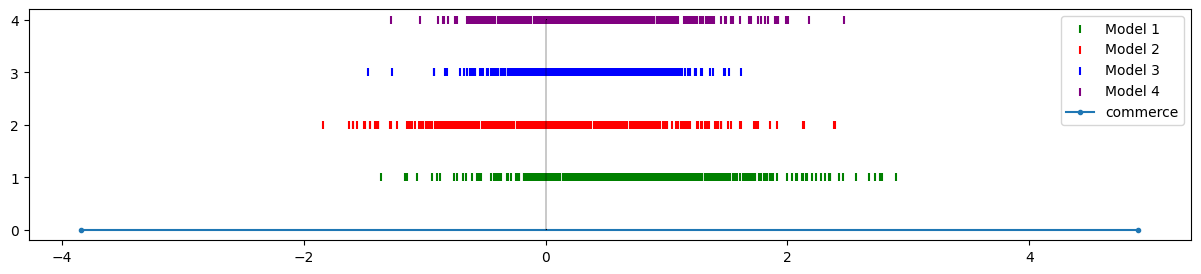
\includegraphics[width=\linewidth]{img/context_commerce.png}
      \caption{Target word: Commerce}
    \end{subfigure} \\
    \begin{subfigure}{0.95\textwidth}
      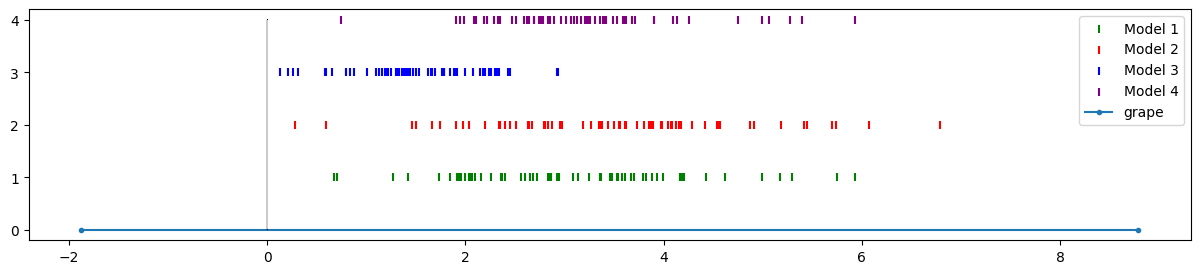
\includegraphics[width=\linewidth]{img/context_grape.png}
      \caption{Target word: Grape}
    \end{subfigure} \\
    \begin{subfigure}{0.95\textwidth}
      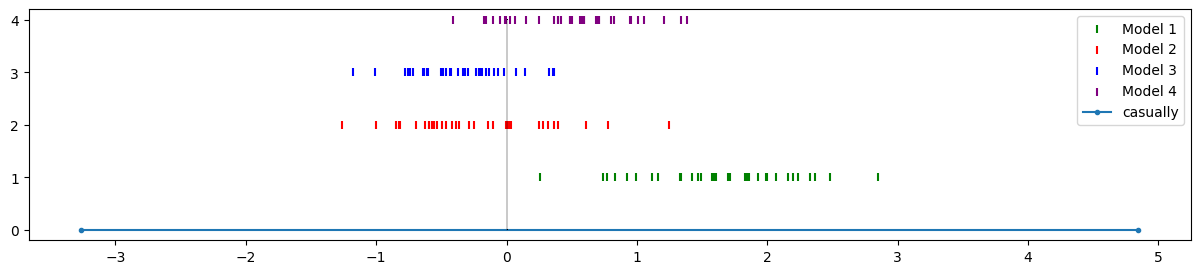
\includegraphics[width=\linewidth]{img/context_casually.png}
      \caption{Target word: Casually}
    \end{subfigure}
  \end{tabular}
  \caption{Context projections onto the selected target words, for the final models of all versions}
  \label{tab:context_proj}
\end{table}

We show the results for the final models of each version, using 3 test words, in Table \ref{tab:context_proj}. We pick the words "\textit{commerce}", "\textit{grape}", and "\textit{casually}". In the figures, we use the names "Model 1", "Model 2", "Model 3" and "Model 4", for the base model, version 15, version 18, and version 26, respectively. Even though it now seems like a projection grouping is relatively more distinguishable, we still fail to point out distinct clusters. 

\section{Comparative evaluations of top four performers}

Now we put our models head to head with some other well-known models pre-trained on very large corpora. We test our models on popular evaluation tests and use standardized evaluation datasets for it. We compare and visualize the results. By the end of this section, we will have a better understanding of the abilities and potentials of our 3rd-order model idea, compared to what is commonly considered "good" in the literature.

\subsection{Tasks and datasets}
\label{sec:tasks_datasets}

To evaluate the abilities of our models from different perspectives, we have chosen three different tasks to perform and several datasets for these tasks as standards. First, we conduct our evaluations in similarity and relatedness tasks, measuring for a given pair of words, how is the level of similarity calculated using our models compared to human judgment. Then we move to word analogy, where the semantic relationships of words are modeled in higher order, and we see if our models are fit for capturing these relationships. Finally, we designed a new evaluation, in which we check if our models are actually able to distinguish different word senses for the same word, given their contexts. This is a new task performed even for the standard models, we produce a new dataset for it and measure the scores achieved by both our models and the standard ones.

\subsubsection{Spearman's Rank Correlation Coefficient}

Before we go any further, we should first introduce the \textit{Spearman Correlation}. Named after its creator Charles Spearman, the Spearman correlation is a popular method for measuring how well the relationship between two variables can be described, using a monotonic function. It is related to but differs from its premise, the Pearson correlation, which examines linear relationships. The Spearman correlation is non-parametric, making it a better choice for variables with non-linear associations. By ranking the data, Spearman correlation measures the degree to which one variable's values change concerning another variable's values. It is a very handy tool for exposing underlying patterns and relations within the dataset. 

The Spearman correlation $\rho$ is calculated by first ranking the values of the two variables and then applying the following formula:

\[
\rho = 1 - \frac{6\sum d_i^2}{n(n^2 - 1)}
\]
\noindent
where $n$ is the number of data points and $d_i$ is the difference between the ranks of corresponding values in the two variables. The result ranges from in $[-1, 1]$, where $-1$ indicates an inverse relationship, $0$ represents no linear relationship, and $1$ implies a perfect direct relationship between the variables.

\subsubsection{Similarity and relatedness}

In this type of evaluation, we take as a reference a dataset containing a set of word pairs, and similarity (or relatedness) scores assigned to them by human annotators. Depending on the dataset, these scores are distributed in different ranges, such as $[0, 10]$, or $[0, 4]$. The similarity score tells us how similar are the meanings of two words, while relatedness measures the relatedness of these two meanings. For example, the words "\textit{car}" and "\textit{bus}" can be considered similar, given that both are the names of some sort of vehicle. On the other hand, the words "\textit{car}", "\textit{bus}" and "\textit{road}" are considered related, considering that they refer to related concepts. In essence, similarity is about the "is a" relation, meanwhile, relatedness is a more general concept, and can be expressed with an "is about" relation. Some datasets draw strict lines between these two terms, awarding one relation and penalizing the other.

This type of evaluation is perhaps the most standardized way of assessing the word representations intrinsically, probably because of the ease of computation, rapidness of implementation, and large community support with a variety of existing human-annotated similarity datasets. Also, considering that it is the method that one is most likely to find in any word embedding model publication, it provides a valuable benchmark to understand how a new model ranks amongst others. However, it definitely comes with its weaknesses, and we find them investigated thoroughly in the article \cite{sim-problems} where the authors analyze when and why this technique may yield unreliable and perhaps meaningless results. We now list what are some of the shortcomings of this approach and briefly mention their reasons. 

\begin{itemize}
    \item Human annotations of word similarity standards are subjective, and this is apparent even though most of the standardized datasets rely on recruiting of large group of annotators to cope with it.
    \item The majority of word embedding models presented are selected among their variants considering their performance on this task. But one should note that the selected model can be implicitly overfitting the used standard, and might fail in any other. 
    \item Even though we have implementation tricks to deal with this effect, we still cannot deny that word embedding models are sensitive to word frequencies in the training corpus. This will definitely impact how a model performs on over and underrepresented words in the evaluation set. In this case, it will be hard to defend that the obtained accuracy will reflect the true quality of the training mechanism and the produced embeddings.
    \item As described in \cite{sim-problems2}, word similarity-based judgments of embeddings rarely correlate with how well they serve their function in downstream \ac{NLP} tasks, such as text classification, parsing, and sentiment analysis.
\end{itemize}

We keep these in mind but still value this technique as a good indicator of how well a word embedding model learns about word semantics. We assess our vectors using this method, but also pair it with other sorts of assessments.

We followed the mechanism introduced in \cite{glove}, and built a testing mechanism similar to theirs. What we do is, for each word pair contained in the dataset, we calculate the cosine similarity using the vectors in hand, put the values for all pairs in a single list, and calculate Spearman's rank correlation coefficient of this list and the human scores provided in that dataset. We omit a word pair if at least one of the two words is not represented by the embedding model. This way, we understand how well our model ranks the similarities of these pairs in a similar way as the human annotators do.

We again consulted \cite{glove} to find out what are the common standards used for this purpose. In the end, we picked 3 of the datasets mentioned in this paper, and additionally find one ourselves. These datasets and their brief descriptions are provided in the following.

\begin{itemize}
    \item \verb|WordSim-353|: It is a quite popular similarity and relatedness benchmark, containing 353 samples annotated by human annotators \cite{wordsim}. The dataset contains annotations made by two annotators, and also similarity and relatedness gold standards. We have used those two gold standards for our evaluations. The similarity gold standard contains 203, and the relatedness gold standard contains 252 word pairs. We ran our evaluation on those two sets separately and also included the average score of two in our tables.
    \item \verb|Stanford Rare Word (RW)|: It is a word similarity dataset put together by a team of researchers from Stanford University in 2012 \cite{rare_word}. This dataset specifically focuses on the rare words (avoiding the "junk" words as they call them), containing 2034 word pairs.
    \item \verb|RG-65|: Named after its creators Rubenstein and Goodenough, and the number of contained word pairs (perhaps also the year of release), RG-65 is yet another word similarity benchmark that is widely utilized \cite{rg65}. The annotations are the averages of judgments made by 51 subjects, with scores ranging from 0 to 4.
    \item \verb|SimLex-999|: It is a gold standard resource genuinely for word similarity rather than relatedness. What we mean by this, is that this dataset contains scores rewarding pure similarity, so that word pairs that refer to associated concepts but are not actually similar have a low rating \cite{simlex}. It was annotated by 500 paid native English speakers and contains exactly 999 word pairs. To make things clearer, Table \ref{tab:simlex} shows an example given in the dedicated website \footnote{\url{https://fh295.github.io/simlex.html}}.
\end{itemize}

\begin{table}[h]
\centering
\begin{tabular}{|
>{\columncolor[HTML]{EFEFEF}}c |c|c|}
\hline
\textbf{Pair} & \cellcolor[HTML]{EFEFEF}\textbf{Simlex-999 rating} & \cellcolor[HTML]{EFEFEF}\textbf{WordSim-353 rating} \\ \hline
\textit{coast - shore} & 9.00 & 9.10 \\ \hline
\textit{clothes - closet} & 1.96 & 8.00 \\ \hline
\end{tabular}
\caption{SimLex-999 versus WordSim-353}
\label{tab:simlex}
\end{table}

\subsubsection{Word analogy}

Word analogy-based evaluation is a method commonly used to examine the quality of word embeddings. For three words $a$, $b$, and $c$, the model is expected to predict
\begin{displayquote}
\centering
What is to $c$, as $b$ is to $a$?
\end{displayquote}

Word analogy datasets contain lines of questions in this format. For example, one line from such a dataset could be, "\textit{Italy, Euro, Turkey, Lira}". For each line, given the first three words, the model tries to guess the fourth one. These questions assess the model's ability to capture semantic relationships of words in a higher order than the similarity-based evaluations.

The calculation of the analogy-based performance of models is very straightforward. It is the ratio of the number of correct answers to the total number of analogies in the evaluation dataset. An answer is considered correct only in the case of exact correspondence of the model prediction and the fourth word in the analogy according to the benchmark. More formally, 

\[
\mathit{Analogy Score} = \frac
{\sum_{(a, b, c, d)\, \in\, D}\quad \mathit{match}(a, b, c, d)}
{|D|}
\]
\noindent
where 
\begin{itemize}
    \item $D$ is the full set of analogies in the dataset,
    \item $(a, b, c, d)$ is a line from $D$,
    \item $\mathit{match}(a, b, c, d)$ is defined as:
\end{itemize}

\[
\mathit{match}(a, b, c, d) = 
\begin{cases}
1 & \text{ if } \mathit{pred}(a, b, c) = d \\ 
0 & \text{ if } \mathit{pred}(a, b, c) \neq d 
\end{cases}
\]
\noindent
where $\mathit{pred}(a, b, c)$ is the model's prediction of $d$ given the first three words. The model's prediction of the fourth word is produced by a fairly simple logic:

\[
w_p = w_b - w_a + w_c
\]
\noindent
where $w_a$, $w_b$, $w_c$ are the representations of the words $a$, $b$ and $c$ according to the model. The model's prediction about the word $d$ is the word $p$, whose representation has the highest similarity with the vector $w_p$ obtained in the above equation. This similarity is measured through the cosine similarity.

We followed exactly this method but also paired it with another version in which we obtained the word $p$ given the vector $w_p$ using the Euclidean distance instead of cosine similarity.

As for the reference dataset, we use the dataset provided in \cite{w2v}, containing 19,557 lines of analogy questions.


\subsubsection{Word Sense Distinction}

Since the beginning of our study, we have always been curious about whether or not we can actually produce a model that organizes the vector space in a way that we can pick apart different contexts of a word. This would enable us to tell given two occurrences of a word, based on the contexts it appears in, if the word senses are the same or not.

The evaluation we are about to describe is designed exactly for this purpose. We call it "Word Sense Distinction", and we use a custom dataset in a very specific format. Our task is closely related to but differs from \ac{WSD}, which is a very well-known concept in the field of \ac{NLP}. In our case, we are interested in telling apart different word senses the same word might have in two different occurrences. Meanwhile, \ac{WSD} also involves correctly identifying which of the possible senses the word takes in the given context.

For this task, we developed our custom dataset. We call this dataset "Sense-Contrast Dataset"\footnote{Available at \url{https://github.com/aonurakman/SCD}}, and we produced it with the assistance of ChatGPT (version 4), which is an \ac{AI}-supported chatbot based on OpenAI's latest large language model, \verb|GPT-4| \cite{gpt4}. 

Following is the prompt we fed into ChatGPT.

\begin{lstlisting}[numbers=none, caption=Prompt used in the generation of Sense-Contrast Dataset]
Generate a 100 lines dataset, each line should be formatted as: 

word; sentence with the word in sense1; sentence with the word in sense2; 1 if sense1 is the same with sense2 else 0

Here are 2 lines as an example:

* bat; she hit the ball with a bat towards the base; rabies is commonly found in bats; 0
* car; should I go there by car or take a bus; he bought a new car from germany; 1

Requirements:

* Do not use punctuation except for the apostrophe.
* Everything must be lowercase.
* Samples with the same word senses and samples with different word senses should be balanced. In other words, there should be 50 samples for both cases.

Optional:

* Try to construct each sentence using 6-8 types.
* Try to place this word somewhere in the middle of the sentence.
* Try not to use too many stopwords.
\end{lstlisting}

ChatGPT provided us with a quite satisfactory answer, providing exactly 100 lines in the requested format. However, it was suffering from repeating lines, incorrect labeling, and very shallow sentences. Because of this, we manually fixed some of the samples as needed, and rewrote some of the lines altogether. In its final form, the dataset was ready to use.

As said in the prompt, this dataset contains 100 samples, each formatted as:

\begin{verbatim}
w;s1;s2;c
\end{verbatim}

\noindent
where

\begin{itemize}
    \item \verb|w| is a word.
    \item \verb|s1| and \verb|s2| are two sentences, containing w.
    \item \verb|c| is the label, which is $0$ if the sense of \verb|w| is the not same in both sentences, $1$ otherwise.
\end{itemize}

Here are two lines from this dataset:

\begin{lstlisting}[numbers=none, caption=Examples from Sense-Contrast Dataset]
leaves;he swept the leaves off the sidewalk;the plane leaves at ten in the evening;0

bowl;she poured cereal into a bowl;this bowl is too small for serving salad in it;1
\end{lstlisting}

We also developed a process to use this dataset to calculate a score for a given model. Step by step,

\begin{itemize}
    \item For each line in this dataset, we collect every other word except \verb|w| from both sentences.
    \item We discard a sample if at least one of the sentences has no words included in the model's embedding dictionary.
    \item We calculate the orthogonal projections of the embeddings of these words onto the embedding of \verb|w|.
    \item We normalize these projections using the length of the sentence they belong to.
    \item We calculate an average projection for each sentence.
    \item We calculate the absolute difference between the average projections of two sentences. 
    \item If the label \verb|c| is $1$, we add this value to \verb|positives|, otherwise to \verb|negatives|.
    \item \verb|positives| and \verb|negatives| are divided by the number of samples with $c=1$ and $c=0$, respectively.
\end{itemize}

In the end,  The final score $S$ of a model is,

\[
S = negatives - positives
\]

By definition, this metric ranges in $[-2, 2]$. The interpretation of this score is not straightforward. A non-positive score or a score near $+2$ is considered unideal. The ideal \verb|positives| value is $0$, while the ideal \verb|negatives| value is in $(0, 1]$. For a score that achieves our context hyperplanes objective, we would expect a score ranging in $(0, 1]$. We also developed another version of this process, in which we use cosine similarity instead of orthogonal projections.

\subsection{Reference models}
For the tasks we described, we also use some other models pre-trained on some large-scale corpora, so that we can have a comparison to the state-of-the-art. We picked two embeddings from perhaps the most well-known models, which are trained on corpora that are dramatically larger than our training dataset. We found these embeddings in Gensim's data storage\footnote{\url{https://github.com/piskvorky/gensim-data}} and downloaded them using their downloader \ac{API}. The models are described in the following, which are identified by the names used in the Gensim storage repository.

\begin{itemize}
    \item \verb|word2vec-google-news-300|: A \ac{CBOW} model trained on a partition of the Google News dataset, which contains about 100 billion words\footnote{For details, see \url{https://code.google.com/archive/p/word2vec/}}. The model contains 300-dimensional vectors for 3 million words and phrases. The phrases were obtained using a simple data-driven approach described in \cite{w2v2}. We will call this model "\verb|word2vec (100B)|" in the upcoming sections.
    \item \verb|glove-wiki-gigaword-300|: Pre-trained vectors on a dataset combining Wikipedia (English) 2014 dump \footnote{\url{https://dumps.wikimedia.org/}}  and Gigaword 5 \footnote{\url{https://catalog.ldc.upenn.edu/LDC2011T07}} \cite{gigaword}, containing in total approximately 6 billion tokens \cite{glove}. It has a vocabulary of 400 thousand words in size and 300 in vector dimensions\footnote{For details, see \url{https://nlp.stanford.edu/projects/glove/}}. We will refer to this model as "\verb|GloVe (6B)|".
\end{itemize}


\subsection{Results: Similarity and relatedness}

In Table \ref{tab:similarity-table}, we show side by side the Spearman rank correlations obtained by each model in word similarity/relatedness tasks, using various standards. We present the model names, benchmark names, model vector dimensions, training corpus size, and correlation scores. For the sizes, we use the number of tokens in our training corpus before the subsampling and preprocessing for our models, and the numbers indicated by the creators for the others. In Figure \ref{fig:similarity-plot}, we visualize the results presented in Table \ref{tab:similarity-table}, by stacking model accuracies together for each standard.

\begin{table}[h]
\centering
\setlength\tabcolsep{3pt} % tighten
\begin{tabular}{|ccc|cccccc|}
\hline
{Model} & {Dimension} & {Size} & {WS (Sim)} & {WS (Rel)} & {WS (Avg)} & {RW} & {RG} & {SimLex} \\ \hline
base & 300 & 17M & 0.70 & 0.62 & 0.66 & 0.24 & 0.57 & 0.21 \\
v15 & 300 & 17M & 0.71 & \textbf{0.65} & 0.68 & 0.26 & 0.61 & 0.22 \\
v18 & 300 & 17M & 0.67 & 0.61 & 0.65 & 0.23 & 0.59 & 0.19 \\
v26 & 300 & 17M & 0.69 & 0.65 & 0.68 & 0.21 & 0.57 & 0.22 \\ \hline
GloVe & 300 & 6B & 0.66 & 0.57 & 0.63 & 0.41 & \textbf{0.77} & 0.37 \\
word2vec & 300 & 100B & \textbf{0.78} & 0.62 & \textbf{0.70} & \textbf{0.53} & 0.76 & \textbf{0.44} \\ \hline
\end{tabular}
\caption{Spearman rank correlation on word similarity and relatedness tasks using different benchmarks.}
\label{tab:similarity-table}
\end{table}

\begin{figure}[h]
    \centering
    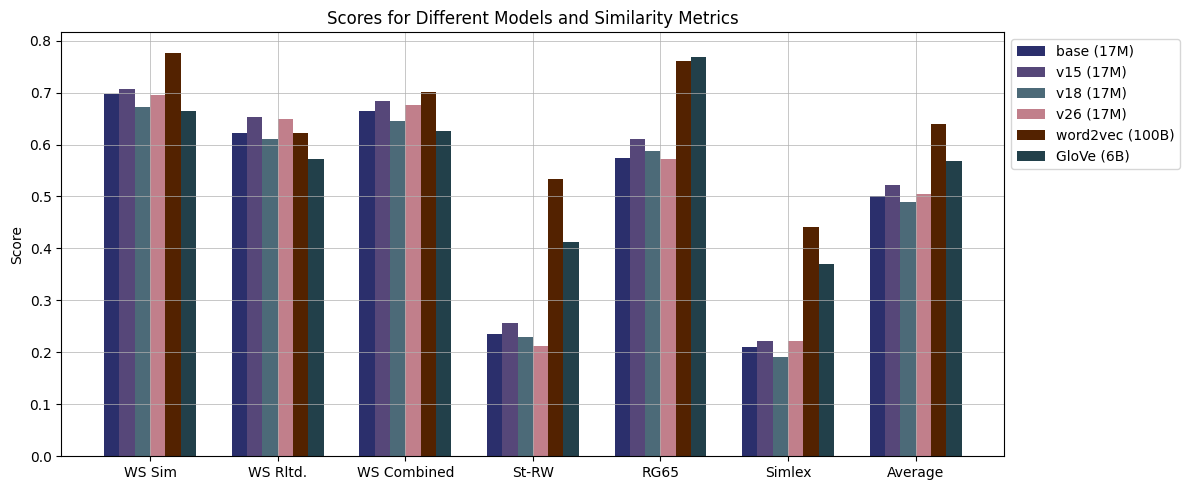
\includegraphics[width=1.0\textwidth]{img/sim_plot.png}
    \caption{Spearman rank correlation on word similarity and relatedness tasks using different benchmarks.}
    \label{fig:similarity-plot}
\end{figure}

We see that our models' performance relative to the pre-trained vectors varies greatly depending on the standard. We see that most of our models overperform GloVe on \verb|WordSim-353| similarity, and dominate both word2vec and GloVe in the relatedness. This is truly impressive, reminding you that we are comparing two pre-trained embeddings to our models that are trained on a tiny fraction of what the former were trained on. 

When we look at the other standards, however, we see a sudden change, and our models get dominated by the other two. For \verb|SimLex-999|, the accuracies are not so far off, but it proves that our model does not rank similarity over any other lexical association between words as well as other models. In the case of \verb|RW| and \verb|RG|, we reason this change merely on the corpora, given that these two benchmarks contain words that are underrepresented in our corpus. Meanwhile, other vectors are based on quite extensive datasets.

\subsubsection{Representation of similarity standards}
We now go ahead and build a base for our reasoning. For each standard, we count how many times each word appears in $V$, where $V$ is our corpora after our preprocessing step. Due to the randomness of our subsampling operation and that it mostly concerns relatively frequent words anyway, we completely disregard it. The average word occurrences for each standard, and the standard deviations of each word occurrence distribution, are given in Figure \ref{fig:occ-avg} and Figure \ref{fig:occ-dev}, respectively. 

\begin{table}[h]
  \centering
  \begin{tabular}{cc}
    \begin{subfigure}{0.47\textwidth}
      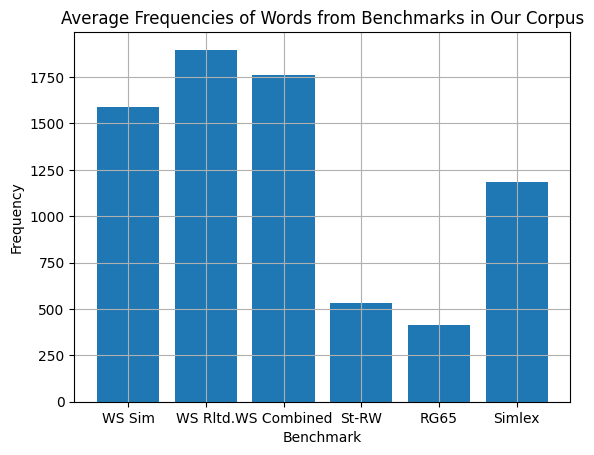
\includegraphics[width=\linewidth]{img/benchmark-occ.png}
      \caption{Average word occurrence of each benchmark}
    \label{fig:occ-avg}
    \end{subfigure} &
    \begin{subfigure}{0.47\textwidth}
      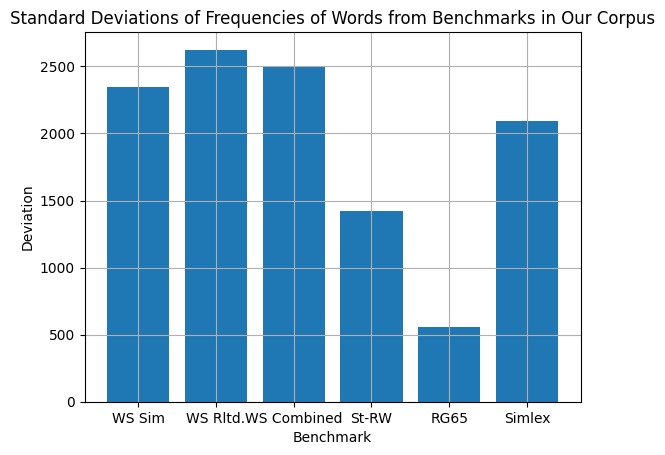
\includegraphics[width=\linewidth]{img/benchmark-std.png}
      \caption{Deviation of word occurrences of each benchmark}
    \label{fig:occ-dev}
    \end{subfigure}
  \end{tabular}
  \caption{Word occurrence statistics of each benchmark in our training corpus}
  \label{tab:occ-stats}
\end{table}

The results presented in Table \ref{tab:occ-stats} prove that the datasets we perform poorly on, except for \verb|SimLex-999|, are indeed underrepresented in our training corpus. Moreover, we see that while the words contained in \verb|WordSim-353| are represented in varying frequencies, the words in \verb|RW| and \verb|RG| are consistently underrepresented. It is unclear if the performance drop stems from this, but we believe this is a very strong factor, if not the main reason.

\subsubsection{Prediction characteristics}

We question if any of the models we use in these assessments stick to a rigid characteristic regardless of the evaluation dataset. This is clearly an undesired case, considering it would diminish the significance of this evaluation mechanism. A model that predicts more or less the same similarity for any given two words would yield good results for a dataset that contains annotations mostly in that range but would perform poorly otherwise. 

\begin{table}[ht]
\centering
\begin{tabular}{|cc|}
\hline
\multicolumn{2}{|c|}{Human Annotations} \\ \hline
\multicolumn{1}{|c|}{Predictions of the base model} & Predictions of v15 \\ \hline
\multicolumn{1}{|c|}{Predictions of v18} & Predictions of v26 \\ \hline
\multicolumn{1}{|c|}{Predictions of word2vec} & Predictions of GloVe \\ \hline
\end{tabular}
\caption{Structure of our charts}
\label{tab:str_charts}
\end{table}

We now share some histograms. We have one figure per similarity standard dataset, and each figure contains histograms of the human annotations in that dataset and the predictions made by each model. We show histograms both for our models and the pre-trained embeddings. We obtain these histograms by binning each value in one of the 10 equally divided bins in the range $[0, 10]$. To make things easier for the reader, we show the blueprint of the charts we are about to share, in Table \ref{tab:str_charts}. 

The histograms for each standard are given in Figures \ref{fig:ws_sim_table}, \ref{fig:ws_rel_table}, \ref{fig:rw_table}, \ref{fig:rg_table}, and \ref{fig:simlex_table}.

\begin{figure}[p]
    \centering
    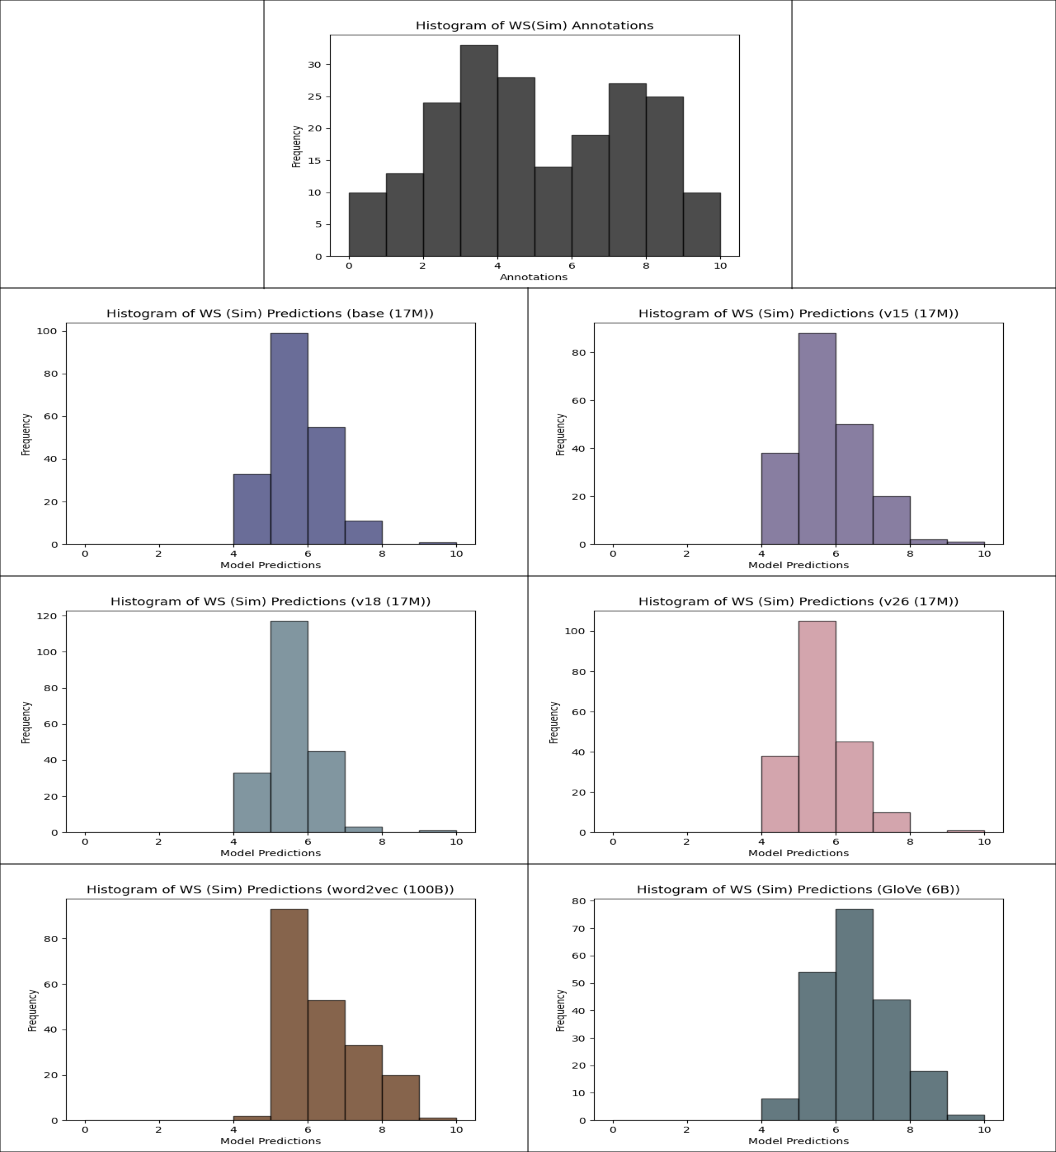
\includegraphics[width=1.0\textwidth]{img/ws_sim_table.PNG}
    \caption{Histograms for WordSim-353 Word Similarity Standard}
    \label{fig:ws_sim_table}
\end{figure}

\begin{figure}[p]
    \centering
    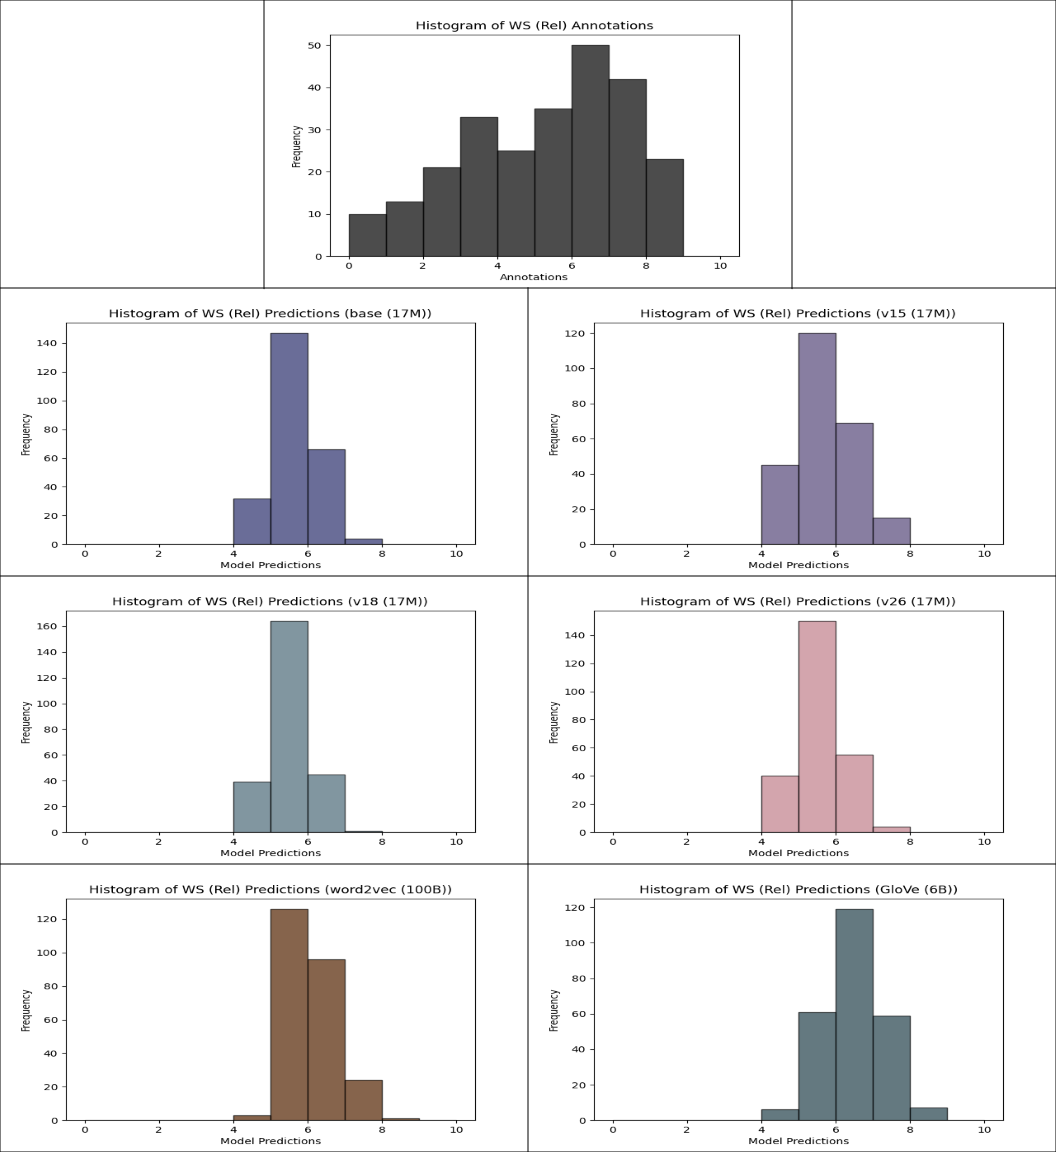
\includegraphics[width=1.0\textwidth]{img/ws_rel_table.PNG}
    \caption{Histograms for WordSim-353 Word Relatedness Standard}
    \label{fig:ws_rel_table}
\end{figure}

\begin{figure}[p]
    \centering
    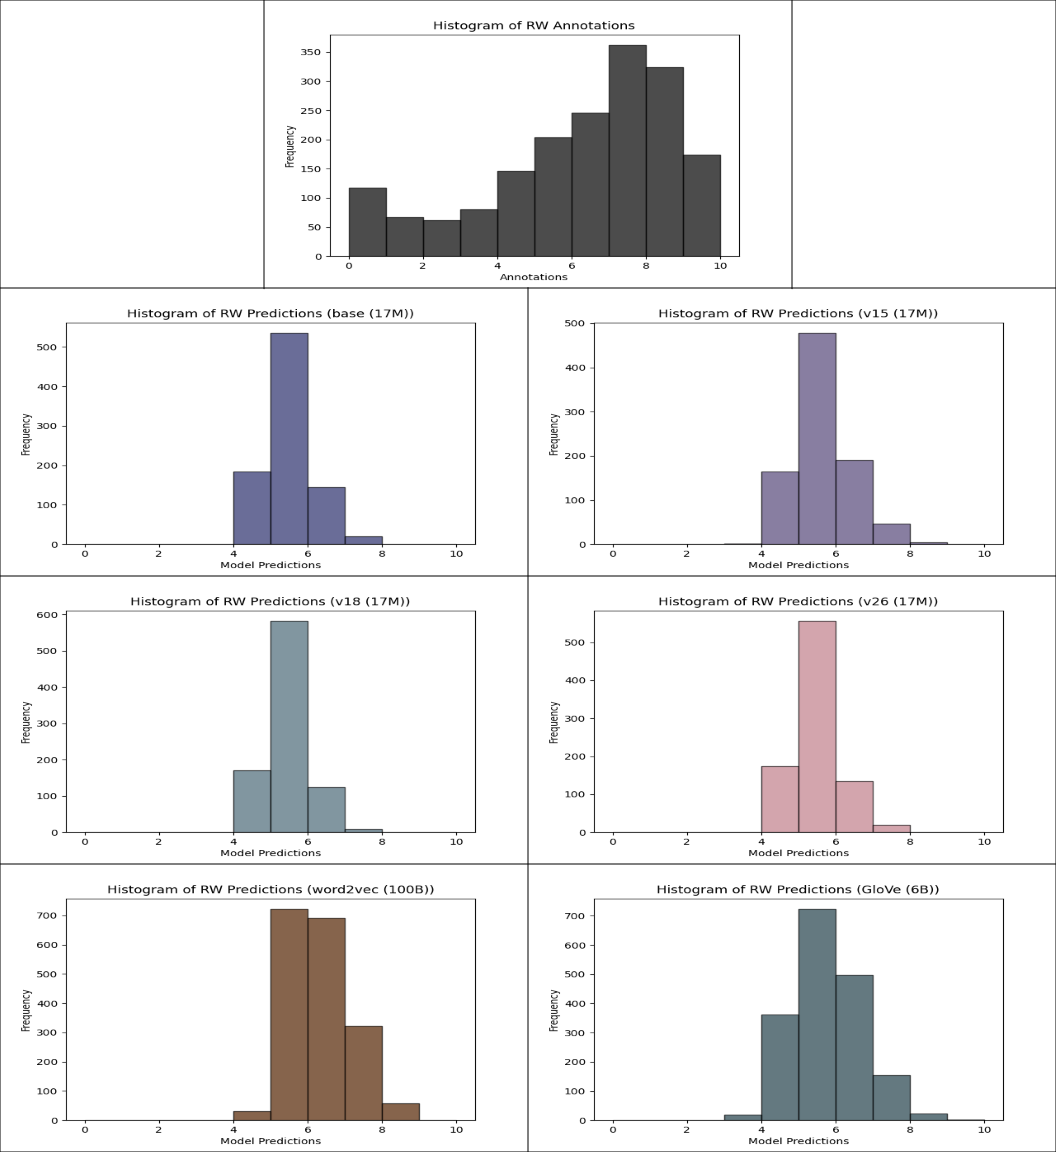
\includegraphics[width=1.0\textwidth]{img/rw_table.PNG}
    \caption{Histograms for Stanford RW Word Similarity Standard}
    \label{fig:rw_table}
\end{figure}

\begin{figure}[p]
    \centering
    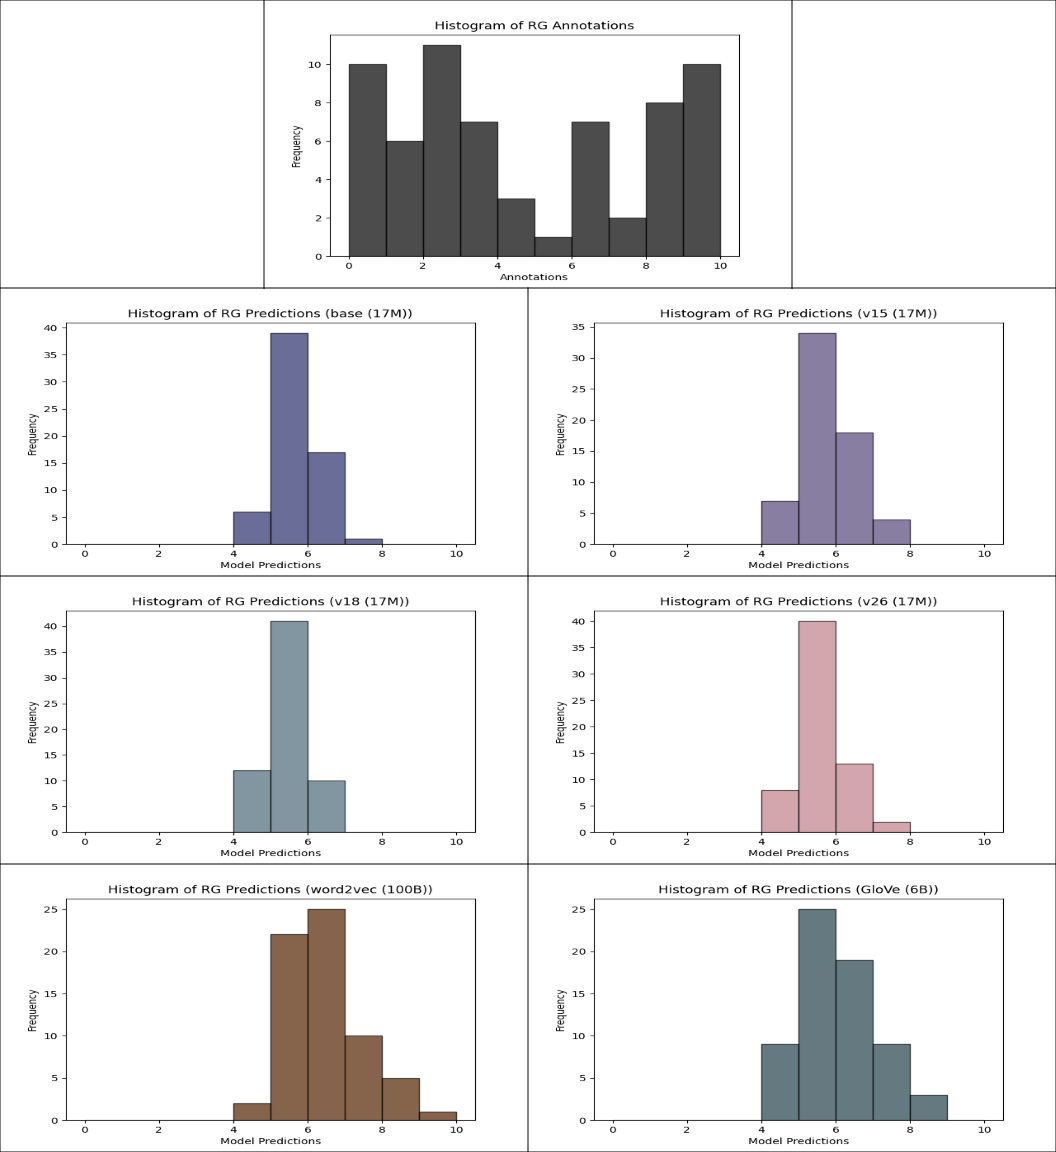
\includegraphics[width=1.0\textwidth]{img/rg_table.PNG}
    \caption{Histograms for RG-65 Word Similarity Standard}
    \label{fig:rg_table}
\end{figure}

\begin{figure}[p]
    \centering
    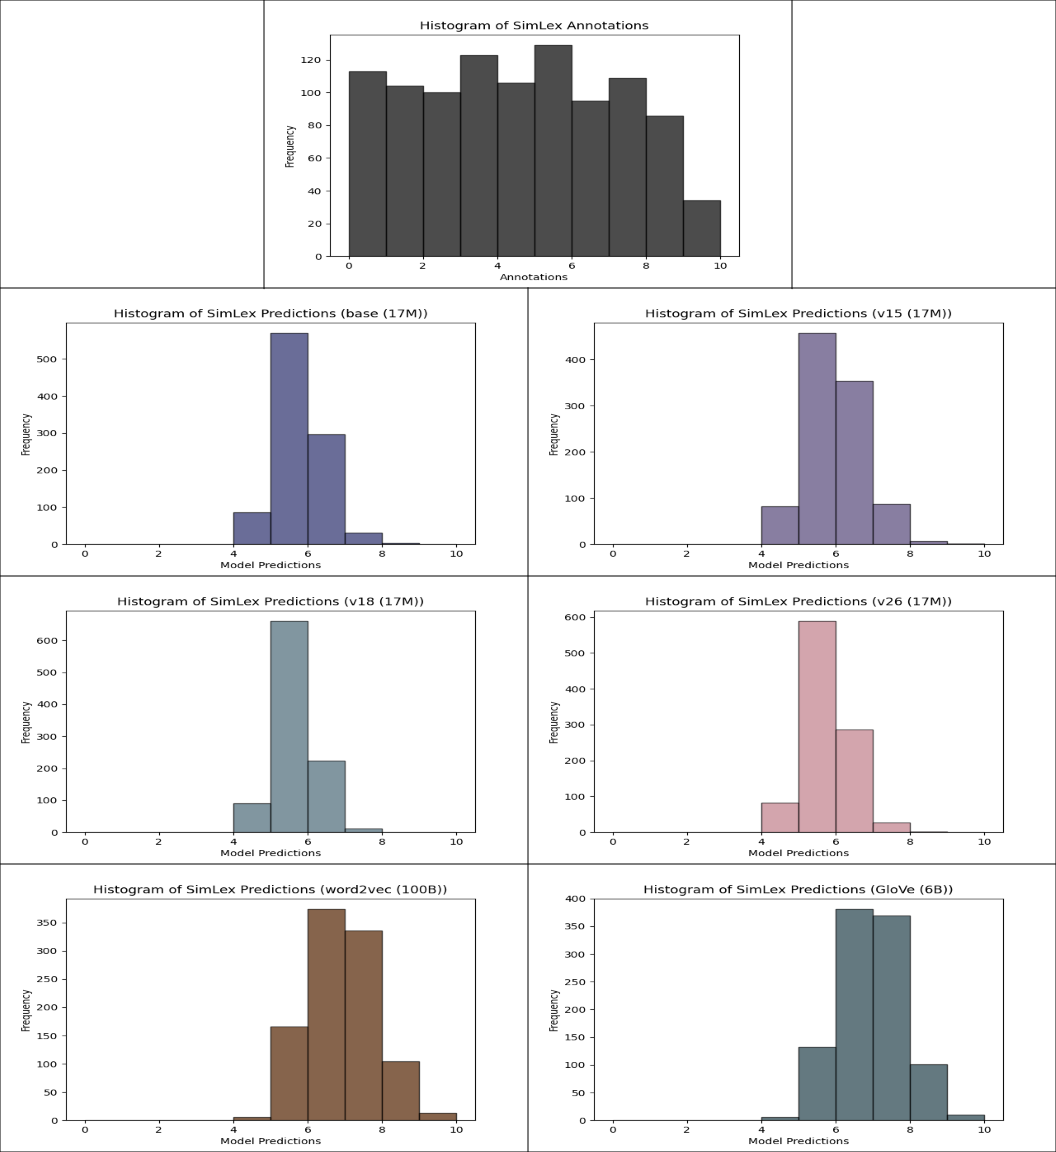
\includegraphics[width=1.0\textwidth]{img/simlex-table.PNG}
    \caption{Histograms for SimLex-999 Word Similarity Standard}
    \label{fig:simlex_table}
\end{figure}


We observe that not only the word embedding models but also the similarity standards differ from each other in terms of the ranges represented in their annotations. For example, we see somewhat of a uniform distribution in \verb|SimLex-999|, but \verb|WordSim-353| datasets favor some ranges while underrepresenting others. This issue is even more apparent in \verb|RG-65| and \verb|RW|. 

As for the models, we see that all the models almost always predict a similarity score from the range $[4, 8]$, regardless of the standard. This may not seem like a bad thing when the standard in hand is \verb|RW|, but it is certainly unideal in the case of \verb|RG-65|, considering the annotation distributions. Overall, we see that all of the models are prone to make predictions from similar ranges, resulting in similar histograms in all figures. But we also see that this issue is not bigger by a margin for our models compared to the standard ones. These findings tell us that our models do not necessarily suffer from this, but also support the points made in the article \cite{sim-problems}, which we discussed earlier in this chapter.


\subsubsection{Closer look: Some predictions}
Finally, we pick two pairs from each standard and present the predictions next to the human annotations. All values are scaled to range [0, 10], and highlight the best predictions for each sample. The results are given in Table \ref{tab:similarity_samples}.

\begin{table}[!ht]
\centering
\setlength\tabcolsep{2.5pt}
\begin{tabular}{|ccc|cccc|cc|}
\hline
\textbf{Pair} & \textbf{Standard} & \textbf{Score} & \textbf{base} & \textbf{v15} & \textbf{v18} & \textbf{v26} & \textbf{w2v} & \textbf{GloVe} \\ \hline
\textit{tiger, cat} & WS (Sim) & 7.35 & \underline {6.27} & 6.18 & 5.64 & 5.59 & \textbf{7.59} & 6.56 \\
\textit{king, cabbage} & WS (Sim) & 0.23 & 4.66 & 4.42 & 4.55 & \underline {\textbf{4.31}} & 5.59 & 4.93 \\
\textit{day, summer} & WS (Rel) & 3.94 & 5.76 & 5.93 & \underline {\textbf{5.46}} & 5.75 & 7.24 & 7.38 \\
\textit{professor, cucumber} & WS (Rel) & 0.31 & 4.79 & 4.80 & \underline {\textbf{4.27}} & 4.48 & 5.28 & 4.73 \\
\textit{imperfection, state} & RW & 0.29 & 5.21 & 5.03 & 5.08 & \underline {4.92} & 5.27 & \textbf{4.41} \\
\textit{friendships, brotherhood} & RW & 7.50 & 5.63 & \underline {5.88} & 5.36 & 5.58 & \textbf{7.32} & 5.87 \\
\textit{cord, smile} & RG-65 & 0.05 & 5.00 & 5.54 & \underline {\textbf{4.79}} & 5.21 & 5.09 & 5.37 \\
\textit{gem, jewel} & RG-65 & 9.85 & 5.59 & \underline {6.02} & 5.22 & 5.61 & \textbf{8.11} & 7.41 \\
\textit{smart, intelligent} & SimLex & 9.20 & 5.27 & 5.14 & 5.08 & \underline {5.94} & 8.25 & \textbf{8.26} \\
\textit{hard, easy} & SimLex & 0.95 & 6.13 & 6.23 & \underline {\textbf{5.75}} & 5.97 & 7.36 & 7.89 \\ \hline
\end{tabular}
\caption{Similarity scores of some word pairs selected from standard datasets and predictions of each model. All scores are scaled to range {[}0, 10{]}. Bold indicates the best estimate of all predictions, and underline indicates the best estimate among our models.}
\label{tab:similarity_samples}
\end{table}

\subsection{Results: Word analogy}

Even though since the very beginning of our study, we did not put any emphasis on the word analogy tasks, we still acknowledge that it is yet another important type of assessment of the quality of static word embeddings in terms of capturing lexical contextual relationships. Unlike our way of thinking, studies like \cite{glove} and \cite{w2v} focus more on the analogy tasks than any other in terms of evaluation techniques. As we described earlier, we built an evaluation process for this task identical to what is considered standard in the literature and also added another version by replacing cosine similarity with Euclidean distance. We show how our models compare to others in both of these versions, in Table \ref{tab:analogy-table}. Then these results are visualized in Figure \ref{fig:analogy-plot}. 

\begin{table}[h]
\centering
\setlength\tabcolsep{4pt}
\begin{tabular}{|ccc|cc|}
\hline
Model & Dimension & Size & Cosine Similarity Based & Euclidean Based \\ \hline
base & 300 & 17M & 0.12 & 0.03 \\
v15 & 300 & 17M & 0.15 & 0.06 \\
v18 & 300 & 17M & 0.06 & 0.01 \\
v26 & 300 & 17M & 0.11 & 0.02 \\ \hline
GloVe & 300 & 6B & \textbf{0.72} & \textbf{0.70} \\
word2vec & 300 & 100B & 0.54 & 0.48 \\ \hline
\end{tabular}
\caption{Accuracies on two versions of the word analogy task}
\label{tab:analogy-table}
\end{table}

\begin{figure}[h]
    \centering
    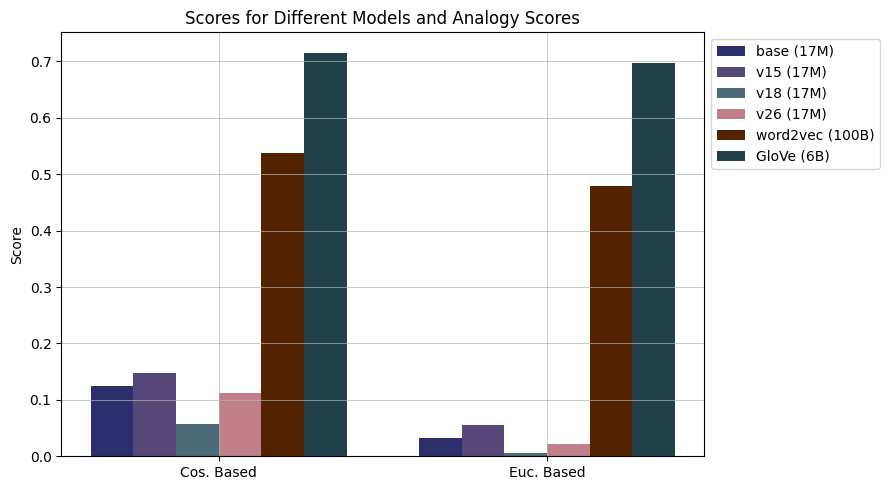
\includegraphics[width=0.8\textwidth]{img/analogy-plot.png}
    \caption{Accuracies on two versions of the word analogy task}
    \label{fig:analogy-plot}
\end{figure}

We observe that our models come nowhere near the standard models in this particular task. We also observe the impressive accuracy achieved by GloVe, demonstrating its versatility, surpassing the word2vec model which is based on a larger corpus by a wide margin. It is difficult to tell how can we reasonably interpret these results, but the following are our estimates of what this poor performance might be stemming from.

\begin{itemize}
    \item \textbf{Validity}: Even though we followed exactly how this task is described in the literature, there is still no solid proof that this is the best way to reveal a word embedding model's abilities. There are several studies in the literature, such as \cite{analogy1} and \cite{analogy2}, criticizing both this way of implementation and the validity of this task altogether. Therefore we suspect the suitability of our models to this way of calculation of word analogy accuracy, but this is a topic to investigate in a follow-up study.
    \item \textbf{The effect of model selection}: In each study for developing a static word embedding model, or any sort of machine learning model, the final version to be presented is selected based on some sort of performance metric. This metric is to comparatively evaluate the performance of a model and the other versions developed in the course of that study. In our case, our emphasis was on the word similarity-based evaluations. Judging from their publications, we suspect that the model selection in other models' developments might be based on word analogy instead. However, even if this is true, it is difficult to argue that this would cause this big of a performance difference. 
    \item \textbf{Suitability}: What makes a word embedding model good at word analogies, or what could cause a model to be bad at it, are questions that are out of the scope of our study. But without any proof that supports our other hypothesis, we can simply assume that our model is not suitable for this task. Therefore we should either admit that there is a lot of room for improvement or not use this metric to assess the quality of our vectors at all.
\end{itemize}

\subsection{Results: Word Sense Distinction}

Dealing with different word senses is not usually a performance indicator for static word embeddings. Static word embeddings, like word2vec or GloVe, are very limited when it comes to handling different senses of words. Static embedding models learn a single vector representation for each type, regardless of context or sense. As a result, they tend to mix up the various senses of a word into a single representation. This is the reason we usually go with dynamic embeddings if the downstream \ac{NLP} task requires a distinction of word senses. Nevertheless, with our custom word sense distinction task, we are looking if it is possible to deal with different word senses using static word embeddings. The results (scaled by 100) are given in Table \ref{tab:word-sense-tab}. The results are visualized for a clearer comparison in Figure \ref{fig:sense-plot}.

\begin{table}[h]
\centering
\begin{tabular}{|ccc|cc|}
\hline
Model & Dimension & Size & Projection Based & Cosine Similarity Based \\ \hline
base & 300 & 17M & 1.67 & 1.58 \\
v15 & 300 & 17M & 2.09 & 1.93 \\
v18 & 300 & 17M & 2.14 & 2.04 \\
v26 & 300 & 17M & 1.22 & 1.23 \\ \hline
GloVe & 300 & 6B & 0.8 & -0.15 \\
word2vec & 300 & 100B & -0.03 & -0.89 \\ \hline
\end{tabular}
\caption{Results of the word sense distinction task (Scaled by 100)}
\label{tab:word-sense-tab}
\end{table}

\begin{figure}[h]
    \centering
    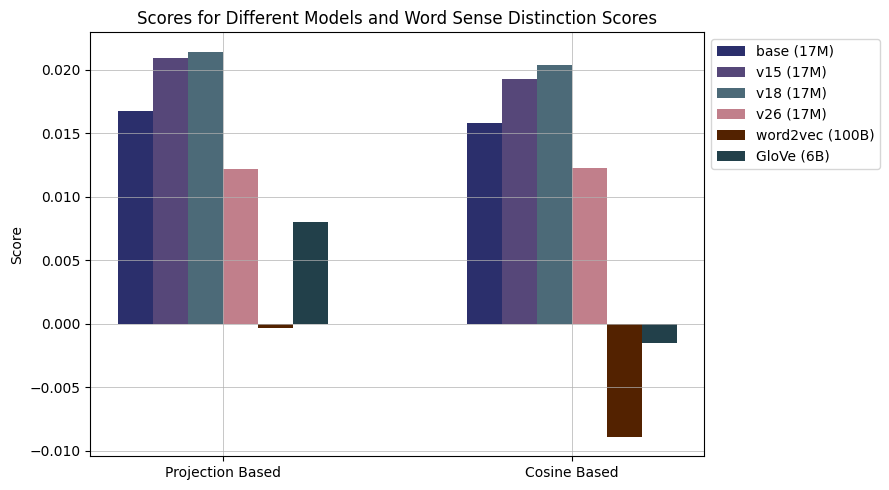
\includegraphics[width=0.9\textwidth]{img/sense-plot.png}
    \caption{Results of the word sense distinction task}
    \label{fig:sense-plot}
\end{figure}

The first observation to make is that our models provide positive valued scores, which is what we were hoping for. The challenge with this metric is that we can only estimate the score that would indicate success, considering that this is a custom process and we do not have a standard for it. Therefore we will consider any positive score as a good indication. 

Secondly, we see that our models dominate the pre-trained ones by a margin. This is also what we were hoping for, but also what we were expecting. We see that according to this metric, the pre-trained models have no ability to tell apart different word senses, while we have this ability in our embeddings.

Thirdly, we see that version 26, which is the one that omits the positive loss $\myscore{+}{w, u_1, u_2}$ from its loss, is our weakest model. We understand the impact of $\myscore{+}{w, u_1, u_2}$ in word sense distinction from this observation. This is perhaps the most valuable observation we made in this experiment since it finally provides a hint about the existence of the context hyperplanes, which we so far failed to prove their existence.

We should note again that this is a fully custom process, which is supported by a fully custom dataset. The evaluation task is not thought in depth as much as other standard evaluation techniques in the literature. Its performance indicator does not have a standard comparison and can be improved to be easier to understand. The dataset is a toy dataset at its best compared to datasets like \verb|SimLex-999|, which is produced by 500 human annotators who are native in English \cite{simlex}. However, we still believe these results are meaningful for showing the sense distinction abilities of our models, especially considering that we did not use this evaluation technique in our model selection procedure.

\newpage

\section{Exploring the effects of training data size on model performance}
\label{sec:data_size}

We mentioned before that it is impressive that our model is comparable to other pre-trained embeddings in some metrics, and we mainly based this on the dramatic difference in the size of the training data. However, in order to claim this, we are very much aware that we need to provide some sort of base by proving that the quality of our embeddings is proportional to the size of the training data we used. 

In this section, we will do exactly that, and investigate the influence of training corpus size on our model's performance. We will share the achieved accuracies of different versions of our base model on different evaluation tasks. These versions differ from each other in terms of the training data we use to train them. We systematically trained our base model using 12.5\%, 25\%, 50\%, and 100\% of our training corpus, maintaining consistent data quality and preprocessing methods across all subsets. 

Instead of slicing a portion of the data and using it, we partitioned the entire corpus into 128 bins and joined the required number of bins by picking them in intervals. This way, we tried to keep the representations of words relative to the size of the dataset somewhat the same.

\subsection{Similarity and relatedness}

Table \ref{tab:sim-scale} shows how the accuracy in word similarity/relatedness evaluations changes with the scale of the training data. Our findings in this test align with expectations, revealing a clear relation between the size of the training data and the model's similarity-based evaluation performance. We then visualize these findings in Figure \ref{fig:sim-scale}.

\begin{table}[h]
\centering
\setlength\tabcolsep{3pt}
\begin{tabular}{|ccc|cccccc|}
\hline
Model & Dimension & Portion & WS (Sim) & WS (Rel) & WS (Avg) & RW & RG & SimLex \\ \hline
base & 300 & 12.5\% & 0.29 & 0.33 & 0.31 & 0.03 & 0.20 & 0.11 \\
base & 300 & 25\% & 0.56 & 0.47 & 0.52 & 0.17 & 0.46 & 0.15 \\
base & 300 & 50\% & 0.61 & 0.59 & 0.60 & 0.19 & 0.49 & 0.17 \\
base & 300 & 100\% & \textbf{0.70} & \textbf{0.62} & \textbf{0.66} & \textbf{0.24} & \textbf{0.57} & \textbf{0.21} \\ \hline
\end{tabular}
\caption{Results of the word similarity/relatedness task, using increasing scales of the corpus}
\label{tab:sim-scale}
\end{table}

\begin{figure}[h]
    \centering
    \includegraphics[width=0.9\textwidth]{img/sim-scale.png}
    \caption{Results of the word similarity/relatedness task, using increasing scales of the corpus}
    \label{fig:sim-scale}
\end{figure}


\subsection{Word analogy}

We now do the same for the word analogy task and put our different-sized models head to head for the word analogy task, and provide the results. Accuracies of our models are provided in Table \ref{tab:analogy_scale}. In Figure \ref{fig:analogy_scale}, we visualize these results for a clear comparison.

\begin{table}[h]
\centering
\begin{tabular}{|ccc|cc|}
\hline
Model & Dimension & Portion & Cosine Similarity Based & Euclidean Based \\ \hline
base & 300 & 12.5\% & 0.009 & 0.008 \\
base & 300 & 25\% & 0.038 & 0.022 \\
base & 300 & 50\% & 0.053 & 0.015 \\
base & 300 & 100\% & \textbf{0.125} & \textbf{0.032} \\ \hline
\end{tabular}
\caption{Results of the word analogy task, using increasing scales of the corpus}
\label{tab:analogy_scale}
\end{table}


\begin{figure}[h]
    \centering
    \includegraphics[width=0.7\textwidth]{img/analogy_scale.png}
    \caption{Results of the word analogy task, using increasing scales of the corpus}
    \label{fig:analogy_scale}
\end{figure}

Except for one incident we observe in the Euclidean-based metric, we see a direct relation between the corpus size and the model accuracy in the word analogy task, proving that as the training data gets larger, our models capture lexical relationships with a better performance.


\subsection{Word Sense Distinction}

Finally, we provide our observations in the word sense distinction set, in Table \ref{tab:sense_scale} (scaled by 100). We visualize these scores in Figure \ref{fig:sense_scale}.

\begin{table}[h]
\centering
\begin{tabular}{|ccc|cc|}
\hline
Model & Dimension & Portion & Projection Based & Cosine Similarity Based \\ \hline
base & 300 & 12.5\% & 0.55 & 0.58 \\
base & 300 & 25\% & \textbf{2.22} & \textbf{2.20} \\
base & 300 & 50\% & 1.92 & 1.70 \\
base & 300 & 100\% & 1.67 & 1.58 \\ \hline
\end{tabular}
\caption{Results of the word sense distinction task, using increasing scales of the corpus (Scaled by 100)}
\label{tab:sense_scale}
\end{table}

\begin{figure}[h]
    \centering
    \includegraphics[width=0.7\textwidth]{img/sense_scale.png}
    \caption{Results of the word sense distinction task, using increasing scales of the corpus}
    \label{fig:sense_scale}
\end{figure}

This is the only task in which we do not observe a proportion between the dataset size and the model performance. Interestingly, the relation is not inverse either. The best performance seems to be achieved by the model with 25\% in size, and the worst one is the smallest model with 12.5\% in size.

Combining all these observations, apart from the latest one, all of our experiments give us a clear indication of the performance boost relative to the dataset size. Based on these, we find the courage to claim that our model has the potential to achieve much better results, surpassing the standard models in some cases and competing with them in others, when a similar amount of training data is provided.



\section{Analyzing the impact of noise word positioning on model consistency}

So far, all of our models aimed to push the noise projections to the left side of the context projections along the target vector. This seemed to achieve satisfactory results, but now we are curious whether or not we can achieve similar results or better, when we do the opposite and push the noise projections to the right instead.

To investigate this, we kept everything the same but altered just one thing in our base model, so that we obtain this new behavior from the same architecture. The only thing that is changed compared to the original base model is the calculation of the projection difference $D$. Using the same notation as Section \ref{sec:neg_loss}, $D$ is now calculated as:

\[ 
D = \frac{e_c(u_3) \cdot e_t(w) - e_c(u_1) \cdot e_t(w)}{\left \| e_t(w) \right \|}
\]

We refer to this new model as \textbf{version 27}. To make sure we get exactly the behavior we desire, we calculated some statistics using this new model. These are the same statistics we calculated for our top-performing models, therefore the interpretation and the comparison will be fairly straightforward.

\begin{figure}[h]
    \centering
    \includegraphics[width=0.9\textwidth]{img/pushleft-stats.png}
    \caption{Statistics computed for the model version 27}
    \label{fig:pushleft-stats}
\end{figure}

Figure \ref{fig:pushleft-stats} shows the statistics computed for this new model. The statistics visualized here are exactly the same ones as in Section \ref{sec:stats}, therefore the reader is advised to refer to that section for the descriptions of these statistics. Opposite of the other models we presented earlier, now we see that as the training proceeds, our context projections get shorter, while the noise projections get longer, at least up to some point. Subsequently, statistic \#4 seems to go down consistently as the learning proceeds, the exact opposite of what we see in the other models. This proves that the desired behavior is obtained. 

\begin{figure}[h]
    \centering
    \includegraphics[width=0.9\textwidth]{img/airport_left.png}
    \caption{For the target word "airport", vector projections in different epochs, using the model version 27}
    \label{fig:airport_left}
\end{figure}

To make things more visual, we show how vector projections change as the training loop iterates, in Figure \ref{fig:airport_left}. This figure is similar to the figures presented in Section \ref{sec:vis_proj}, therefore the reader is advised to go through the descriptions provided there. As for the model performance, we conducted the same evaluations as described in Section \ref{sec:tasks_datasets} on this new model and compared it to the original base model. The exact scores are omitted as they are not so relevant now, and we show the graphs comparing these two models only instead.

\begin{table}[p]
  \centering
  \begin{tabular}{cc}
    \begin{subfigure}{0.9\textwidth}
      \includegraphics[width=\linewidth]{img/sim_v27.png}
      \caption{Word similarity \& relatedness tasks, base model versus version 27}
    \end{subfigure} \\
    \begin{subfigure}{0.8\textwidth}
      \includegraphics[width=\linewidth]{img/analogy_v27.png}
      \caption{Word analogy task, base model versus version 27}
    \end{subfigure} \\
    \begin{subfigure}{0.8\textwidth}
      \includegraphics[width=\linewidth]{img/wsd_v27.png}
      \caption{Word sense distinction task, base model versus version 27}
    \end{subfigure}
  \end{tabular}
  \caption{Evaluations conducted on the model version 27, compared to the base model}
  \label{tab:basev27}
\end{table}

Table \ref{tab:basev27} shows the performance of this new model, version 27, on our set of evaluation tasks, and how it compares to what is achieved in the base version.

These results show that version 27 is almost never able to achieve the exact scores achieved by the base model, but we are fairly close. For the purpose of this section, the latter part is more important for us. We can now say that as long as we separate noise and context projections onto the target vector, our models are able to achieve somewhat similar results, regardless of the direction chosen.



% $\myscore{+}{w, u_1, u_2}$


    %!TEX root = ../main.tex

\chapter{Conclusions and Future Works}
\label{chp:conclusions}

In this chapter, considering everything we discussed up to this point, we will share our vision regarding how can this model be improved and what is left to explore, and then we draw our conclusions. We are hoping to inspire possible further studies on this model and provide a good starting point for them. 

\section{Improvability}

Every decision throughout this study was made by aiming for an efficient utilization of our resources, such as time, computational power, and disk space. These considerations forced us to go with no-so-ideal options from time to time. For instance, in Chapter \ref{chp:experiments}, we repeatedly highlight that the fact that our model can even compete with other pre-trained vectors in some metrics is quite impressive, considering that the data we used for training is significantly smaller. Then instead of training our models using similarly scaled data, we put forward an experiment to show that our models benefit from the larger-sized training data in Section \ref{sec:data_size}. Obviously the former would be more convincing, but we did not have memory capable of handling that big of data, and we did not even have access to a high-performing GPU for the durations mentioned in \cite{w2v2}. Another example is the explorations of hyperparameter configurations space or other design choices, which we did our best given our limited time, but surely there is way more to see than the versions described in Section \ref{sec:variants}. For instance, we could not explore the effects of other values of learning rates and decay rates, or different optimizers, due to the time constraints.

Therefore there is definitely more to explore, and some of these new things to try are most likely will yield better performances. Now we list some of the things that we did not make it in the duration of our study, but can potentially improve the model performance or provide new insights if applied.

\subsection{Change of training data}

The observations in Section \ref{sec:data_size} allowed us to believe that our model can indeed perform better if more training data is provided. Coming from this, we can argue that training our model using a larger training dataset is definitely worth trying. However, we should note day this will require significantly higher memory and perhaps a day-long training time. Using a large corpus, such as a recent version of Wikipedia Dumps or Google News, the vocabulary will be much more extensive and the words will be observed in many different contexts.

\subsection{Data partition}

Our focus in this study was to train a word embedding model on a sufficiently large dataset and observe its characteristics comparatively to the standard models. We also dealt with time and computation limitations. Therefore we were not interested in exploring the smarter ways to partition our data into training and validation sets, nor using a test set to test our training performance. For future studies, where the objective is to produce a set of word embeddings to compete with the state-of-the-art models, one should consider these factors in more depth. For instance, the validation split can be done more mindfully, perhaps using a technique like K-Fold Cross Validation. Also, an additional layer of evaluation can be implemented, using a test partition from the training set. The results of this sort of evaluation would not tell us much about the model's performance on any intrinsic or extrinsic assessments, but it would give the developers a clearer picture of which model learned the most efficiently from the training data, compared to its variants.

\subsection{Dealing with overfitting}
We see clearly in our learning curves that our models overfit the training data, just after a few epochs. This may be caused by several things, such as the choice of the dimensionality of the vector space, given the size of the training data. It is not possible to estimate what would happen if the training data were selected differently, but in case it is again observed in future studies, the designers shall consider how to deal with this issue so that the final product will generalize better. One way to cope with this is a regularization technique called \textit{Early Stopping}, in which the training is finalized earlier than the set number of epochs if the performance on the validation set does not improve or gets worse (based on a predefined \textit{tolerance}) for a predefined number of steps.

\subsection{Learning rate decay}
Learning rate scheduling is an approach that allows us to systematically decay the learning step size as the training iterates. This is employed in order not to diverge from the found solution, and converge to a local minima that otherwise we would not be able to reach with a large step size. Decreasing the step size might make it slower to reach a solution. However, we believe that this technique is highly suitable for our case, given that our model already starts to overfit from very early on. This technique is something we briefly tried in our version 2 (see Section \ref{sec:variants}), and it provided some promising results. However, we believe that our attempt was not sufficient to fully explore the potential benefits.

\subsection{Stopword removal and subsampling}
As we described earlier in Section \ref{sec:preprocessing}, we remove an extensive set of stopwords from the corpus in the preprocessing step. After, we also apply the subsampling operation, removing some occurrences of frequent words, in order to balance the representations. We believe this will enable us to capture more contextual relationships of words, by removing the words that fill up the context windows without carrying much information. However, our way of doing it is rather strict, and this was needed to further improve the training efficiency. Therefore further studies are strongly encouraged to loosen up this procedure to see if preserving some of these words will improve the model performance.

\subsection{Embedding dimensionality}
We chose 300-dimensional vector space to embed our words, as it is a widely used number in the literature. However, given that our training data is significantly smaller than how it is in most of the studies, if we had gone with a small dimension selection for our smaller vocabulary, perhaps we could have prevented overfitting. Similarly, in the case of training our model with a larger corpus, perhaps more dimensions would allow our third-order model to encode more information.

\subsection{Normalization in loss function}
We observe that as the training proceeds, our vectors get longer and longer. We had no reason to believe that this might influence the model performance either negatively or positively. However, further experiments can be conducted to investigate this effect, or better, the vector projections can be normalized using the target vector length to see the change in the model performance.

\subsection{Understanding the model behavior}

As we described in Section \ref{sec:stats} and Section \ref{sec:vis_proj} we spared a significant amount of time for understanding how our models learn word representations as the training proceeds. However, we believe that we still did not fully explain our model's behavior. Understanding our model in depth might seem redundant as long as we produce high-quality embeddings, but we trust that this is vital for making it even better or inspiring further studies and new models. We did not present in this dissertation, but we also attempted to visualize our embeddings in three dimensions using dimensionality reduction techniques. However, these efforts suffered from loss of information, and the final results were not as expressive as we hoped. Finding new visualization techniques, or simply a more in-depth thought process, might provide new material for improving our model or prove its advantages over other standardized models.

\subsection{Downstream NLP tasks}
We decided to work with intrinsic evaluation techniques, which are to assess the quality of word embeddings as they are, with respect to some provided ground truth. This is the most straightforward way to get an idea about the quality of a word embedding model but by no means is it the only way. Alternatively, we could have opted to employ extrinsic methods, which involve evaluating word embedding vectors or comparing two sets of embeddings by integrating them into downstream \ac{NLP} tasks and subsequently evaluating the resultant systems. We cannot argue that this way would provide more reliable results, but this multifaceted approach enables a more comprehensive understanding of the versatility and effectiveness of word embeddings within broader \ac{NLP} contexts. 

We are optimistic that our model is capable of yielding even more impressive results for tasks that demand finer contextual distinctions. However, we should note that our model may not offer the same level of plug-and-play convenience as others. Just like we did in designing the evaluation task "Word Sense Distinction", designers should be aware of the distinct nature of our vectors and design an appropriate method to use these vectors to their full potential.

\newpage
\section{Final remarks}

In this dissertation, we aimed to present our work as a self-contained and comprehensible entity. First, we tried our best to give the reader a theoretical background before proceeding to our work, talking about more generalized concepts like Machine Learning and Natural Language Processing, and then focusing on word embeddings and some of the state-of-the-art models. Later in Chapter \ref{chp:design}, we described our idea and how we mathematically formulate it. Following this blueprint, Chapter \ref{chp:implementation} was about how we programmed our training mechanism. We then evaluated our products and discussed our findings in Chapter \ref{chp:experiments}, providing some numbers and visuals to make things clear. Finally, we provide our ideas for further explorations and remarks in this chapter, hoping to inspire efforts to improve this model. We tried to balance different aspects of this project in our descriptions, leveraging formulas, code blocks, plots, and of course, plain text, to make things as understandable as possible for readers from different backgrounds.

We are glad and excited to present a fresh perspective on a long-standing problem within the field of \ac{NLP}. Given the unique nature of our approach, which lacks direct benchmarks from prior studies, we acknowledge that we needed to be careful while designing evaluation processes and commenting on the results, as it is not easy to validate them. Nevertheless, we tried our best to remain as objective and rigorous as possible, fairly assessing our models and highlighting their weaknesses as much as their strengths.

We spent quite a bit of time brainstorming and literature reviewing, in order to explore what kind of experiments we could conduct to effectively visualize our vectors and how can we assess them. We picked some of the most popular studies in this domain and found their most compatible models, in order to provide a benchmark for our products. We aimed to effectively demonstrate what has now been achieved and what can still be improved.

Our models produce vectors that can capture contextual relationships of words and take a fraction of data to train compared to other standard models. We believe there is still more to explore and interpret about this approach, but we are happy to put forward a new perspective on static word embeddings, which are inherently thought to be rather rigid and limited. Today's latest \ac{NLP} advancements are based on higher-level concepts such as large language models, question-answering systems, or automatic translation. However, static word embeddings still hold relevance in today's NLP advancements by offering efficiency, simplicity, and as we believe, improvability.

As we now conclude our remarks, we would like to emphasize the significance of continuous advancement in the foundational elements of a system, in order to overcome what was previously thought to be a limitation. It is important to find new ways to build the next biggest and the most impressive skyscraper, but innovating how we produce bricks can always unlock entirely new possibilities. Similarly, we believe that the advancements in static word embeddings can offer unthinkable advancements in the higher-level \ac{NLP} tasks. With this in mind, we hope that the work we presented here is useful for enhancing the way we produce static word embeddings today, or inspirational for those who are looking for new ways to produce them.




    %%!TEX root = ../main.tex

\chapter{Cheat sheet}
\label{chp:cheat}


% -----------------------------


Random citation \cite{alecci2021development}.


% -----------------------------


Random footnote.\footnote{\url{https://lucamartinelli.eu.org}}


% -----------------------------


\section{A section}


% -----------------------------


\subsubsection{Example of list}
\begin{itemize}
  \item Item 1
  \item Item 2
\end{itemize}


% -----------------------------


\subsection{A subsection}


% -----------------------------


\subsubsection{Example of acronym}
\ac{NLP}


% -----------------------------


\subsubsection{Example of enumeration}
\begin{enumerate}
  \item Item 1
  \item Item 2
\end{enumerate}


% -----------------------------


\subsubsection{Example of quote}
\begin{displayquote}
Lorem ipsum dolor sit amet, consectetur adipiscing elit, sed do eiusmod tempor incididunt ut labore et dolore magna aliqua.
\end{displayquote}


% -----------------------------


\begin{figure}[ht]
    \centering
    \includegraphics[width=0.5\textwidth]{res/ltunipd}
    \caption{Example of image}
\end{figure}


% -----------------------------


\begin{algorithm}[ht]
    \caption{An algorithm with caption}\label{alg:two}
    \begin{algorithmic}
        \REQUIRE $n \geq 0$
        \ENSURE $y = x^n$
        
        \STATE $y \gets 1$
        \STATE $X \gets x$
        \STATE $N \gets n$
        
        \WHILE{$N \neq 0$}
            \IF{$N$ is even}
              \STATE $X \gets X \times X$
              \STATE $N \gets \frac{N}{2} $  \COMMENT{This is a comment}
            \ELSIF{$N$ is odd}
              \STATE $y \gets y \times X$
              \STATE $N \gets N - 1$
            \ENDIF
        \ENDWHILE
    \end{algorithmic}
\end{algorithm}


% -----------------------------


\begin{equation}
e^{j\pi} + 1 = 0
\end{equation}


% -----------------------------


\tikzset{vertex style/.style={
    draw=#1,
    thick,
    fill=#1!70,
    text=white,
    ellipse,
    minimum width=2cm,
    minimum height=0.75cm,
    font=\small,
    outer sep=3pt,
  },
  text style/.style={
    sloped,
    text=black,
    font=\footnotesize,
    above
  }
}


% -----------------------------


\begin{figure}[ht]
    \centering
    \begin{tikzpicture}[node distance=2.75cm,>={Stealth[]}]
        \node[vertex style=cyan] (Rk) {Righteous Kill};
        \node[vertex style=orange, above of=Rk,xshift=2em] (BD) {Bryan Dennehy}
        edge [<-,cyan!60!blue] node[text style,above]{starring} (Rk);
    \end{tikzpicture}
    
    \caption{Image created with TikZ} \label{fig:T1}
\end{figure}


% -----------------------------


\paragraph{}
Lorem ipsum dolor sit amet, consectetur adipiscing elit, sed do eiusmod tempor incididunt ut labore et dolore magna aliqua. Ut enim ad minim veniam, quis nostrud exercitation ullamco laboris nisi ut aliquip ex ea commodo consequat. Duis aute irure dolor in reprehenderit in voluptate velit esse cillum dolore eu fugiat nulla pariatur. Excepteur sint occaecat cupidatat non proident, sunt in culpa qui officia deserunt mollit anim id est laborum.


% -----------------------------


\begin{lstlisting}[language=Python, caption=Code snippet example]
import numpy as np
    
def incmatrix(genl1,genl2):
    m = len(genl1)
    n = len(genl2)
    M = None #to become the incidence matrix
    VT = np.zeros((n*m,1), int)  #dummy variable

    test = "String"
    
    #compute the bitwise xor matrix
    M1 = bitxormatrix(genl1)
    M2 = np.triu(bitxormatrix(genl2),1) 

    for i in range(m-1):
        for j in range(i+1, m):
            [r,c] = np.where(M2 == M1[i,j])
            for k in range(len(r)):
                VT[(i)*n + r[k]] = 1;
                VT[(i)*n + c[k]] = 1;
                VT[(j)*n + r[k]] = 1;
                VT[(j)*n + c[k]] = 1;
                
                if M is None:
                    M = np.copy(VT)
                else:
                    M = np.concatenate((M, VT), 1)
                
                VT = np.zeros((n*m,1), int)
    
    return M
\end{lstlisting}


% -----------------------------


\begin{table}[ht]
    \centering
    \begin{tabular}{|l|l|}
    \hline
    \textbf{A} & \textbf{B} \\ \hline
    C          & D          \\ \hline
    E          & F          \\ \hline
    G          & H          \\ \hline
    \end{tabular}
    \caption{Table example \label{tab:table-name}}
\end{table}
    
    % Bibliography, appendix, acknowledges, etc...
    \backmatter
\end{document}